\chapter{Numerical solutions of the Ornstein Zernike equations}

 During an internship project in summer 2013 Evgeniy
Ponomarev has implemented the core routine for solving the Ornstein
Zernike equations. This algorithm numerically calculates structure
factors $S(q)$, radial distribution functions $g(r)$ and direct
correlation functions $c(r)$ of a systems with known pair
interaction potential $U(r)$.
\section{Background}
The central part of this package is iterative solution of
Ornstein-Zernike equation \cite{Ornstein1914}. The theoretical background can be found
in great detail in \cite{Naegele2004,Henderson2000,Hansen2013,Bomont2008,Caccamo1996,Likos2001}.
The Ornstein-Zernike equation reads
\begin{align}\label{eq:oz_h12}
    h(\mathbf{r}_{12})&=c(\mathbf{r}_{12})+ \int c(\mathbf{r}_{13}) \rho(\mathbf{r}_3) h(\mathbf{r}_{32})
    d\mathbf{r}_3 + \cdots
\end{align}
where $h(\mathbf{r}_{12})$ is the total correlation function,
$c(\mathbf{r}_{12})$ the direct correlation function (direct effect
of particle 1 on particle 2), $c(\mathbf{r}_{13})$ the in direct
correlation function describing the effect of particle 1 on particle
3 which influences particle 2, and $\rho$ the particle number
density of the colloids, molecules, or atoms that form the liquid.
If the fluid is uniform and isotropic, the Ornstein–Zernike relation
becomes
\begin{align}\label{eq:ozh(r)}
    h(r)&=c(r)+ \rho \int c(\abs{\mathbf{r}-\mathbf{r}'})  h(r')
    d\mathbf{r}' \\
    &= c(r) + \gamma(r) \label{eq:ozgamma(r)}
\end{align}
The basic idea of this equation is that total correlation between
positions of two particles is a combination of their direct and
indirect (through neighboring particles) interactions. The first
contribution to $h(r)$ is the direct correlation function $c(r)$
that represents the correlation between a particle of a pair with
its closest neighbor separated by a distance $r$. The second
contribution is the indirect correlation function $\gamma(r)$, which
represents the correlation between the selected particle of the pair
with the rest of the fluid constituents.

 $g(r)$ is known as the radial or pair distribution  function, which measures the
probability that given a particle at the origin, another particle of
the fluid can be found at a distance $r$ from it. When the distance
separating a pair of particles tends to infinity, the correlations
vanish and $g(r)$ tends to 1. This means that the total correlation
function defined as $h(r)=g(r)-1$ tends to 0. The Fourier transform
$\mathscr{F} \{\}$ of $g(r)$ and $h(r)$ are directly related to the
structure factor $S(q)$ that is experimentally measurable by x-ray
or neutron scattering
\begin{align}
S(q)&=1+\rho \int
\left[g(r)-1\right]\exp\left(-\imath\mathbf{q}\cdot
\mathbf{r}\right) d\mathbf{r}
\end{align}
and
\begin{align}
S(q) &= 1+ \rho  \tilde{h}(q)
\end{align}
where $\tilde{h}(q)=\mathscr{F} \left\{h(r)\right\}$  is the Fourier
transform of the total correlation function $h(r)$, so that
\begin{align}
\tilde{h}(q) &= \int h(r) \exp\left(-\imath\mathbf{q}\cdot
\mathbf{r}\right) d\mathbf{r}
\end{align}
Via inverse Fourier transform $\mathscr{F}^{-1} \{\}$ of the
structure factor the pair correlation function is obtained
\begin{align}
\rho \left[ g(r)-1\right] &=\mathscr{F}^{-1} \left\{S(q)-1\right\} =
\frac{1}{(2\pi)^3} \int \left( S(q)-1
\right)\exp\left(\imath\mathbf{q}\cdot \mathbf{r}\right) d\mathbf{q}
\end{align}
As for $g(r)$ also the direct correlation function $c(r)$ can be, in
principle, derived from experiment as
\begin{align}
\rho c(r) &= \frac{1}{(2\pi)^3} \int \left(1-\frac{1}{S(q)}\right)
\exp\left(\imath\mathbf{q}\cdot \mathbf{r}\right) d\mathbf{q}
\end{align}
or
\begin{align}
S(q) &= \frac{1}{1-\rho \tilde{c}(q)} \label{eq:ozSq}
\end{align}
By Fourier transformation of eq.\ \ref{eq:ozh(r)}, one obtains
\begin{align}
\tilde{h}(q) &= \frac{\tilde{c}(q)}{1-\rho\tilde{c}(q)}
\label{eq:ozhq}
\end{align}
where $\tilde{c}(q)=\mathscr{F}\left\{c(r)\right\}$ is the Fourier
Transform of $c(r)$. In order to determine the two correlation
functions $h(r)$ and $c(r)$ for a given pair potential $u(r)$, eq.\
\ref{eq:ozh(r)} must be supplemented by an auxiliary closure
relation. Furthermore the Fourier transform of eq.\
\ref{eq:ozgamma(r)} in combination eq.\ \ref{eq:ozhq} allows to
write the Fourier transform of the indirect correlation function as
\begin{align}
\mathscr{F} \left\{\gamma(r)\right\} &= \tilde{\gamma}(q)  =
\tilde{h}(q) - \tilde{c}(q) =
\frac{\rho\tilde{c}^2(q)}{1-\rho\tilde{c}(q)} \label{eq:ozg(q)}
\end{align}


 The closure is not complete as long the bridge function is
unknown. Even though the bridge function is exactly defined the
function is an unknown function of interparticle distance and only
approximations can be given. The direct correlation function can be
written in terms of the indirect correlation function, the
inetraction potential and the bridge function as
\begin{align}\label{eq:ozclosure}
c(r)&= \exp\left[ -\beta u(r) +\gamma(r)+B(r)\right] - \gamma(r)-1 \\
    &= g(r)- \gamma(r)-1 \nonumber \\
\mbox{and } h(r)+1=g(r)&= \exp\left[ -\beta u(r)
+\gamma(r)+B(r)\right] \label{eq:ozg(r)}
\end{align}
where $u(r)$ is the pair interaction potential, $\beta=1/(k_B T)$
the inverse temperature, with $k_B$ being Boltzmann’s constant, $T$
is the absolute temperature, $\gamma(r)$ being the indirect
correlation function and $\rho$ is the number density of the
molecules or atoms that form the liquid. $B(r)$ is the bridge
function. The analytic expression of $B(r)$ is, in general, unknown.
Unfortunately, the bridge function has to be approximated in
practice. Though a number of theoretical and simulation procedures
have been derived in recent years in order to get an approximate
estimate of $B(r)$ for different fluid models, the exact bridge
function is not known for any system.

\section{Numerical implementation of the iterative algorithm in \SASfit}

The easiest algorithm for solving the Ornstein Zernike (OZ) equation \ref{eq:ozh(r)} together with the closure equation \ref{eq:ozclosure} is is direct iteration using fast Fourier transformation (see e.g. \cite{Homeier1995}). The solution of the OZ equations is treated as a fixed point problem for the unknown function $\gamma(r)$. In \SASfit the Picard's iteration scheme is implemented:
\begin{enumerate}
\item Guess a starting value for $\gamma(r)$, e.q. set $\gamma(r)\equiv 0$
\item Calculate a bridge function. Many different theories how to calculate the bridge function have been published. A few of them are described in the next section. The bridge function is often expressed in terms of the known potential $u(r)$ and the indirect correlation function $\gamma(r)$, which needs to be determined.
\item Calculate the direct correlation function according to eq.\ \ref{eq:ozclosure}.
\item Calculate the Fourier transform $\tilde{c}(q)$ of the direct correlation function.
\item Use eq.\ \ref{eq:ozg(q)} to get $\tilde{\gamma}(q)$.
\item Calculate the inverse Fourier transform of $\tilde{\gamma}(q)$ to get the new guess for $\gamma(r)$.
\item Compare the new guess of the indirect correlation function with the one used in step 1, i.e. compare $\gamma_\text{new}(r)$ and $\gamma_\text{old}(r)$ at each grid point. If $\Norm{\gamma_\text{new}(r)-\gamma_\text{old}(r)}/\Norm{\gamma_\text{new}(r)} < \epsilon_\text{rel}$ the solution has been found otherwise go back to the first step by using the new $\gamma_\text{new}(r)$ as a starting value and repeat the loop until convergence. \item When the iteration loop has converged calculate $S(q)$ and $g(r)$ according to eq.\ \ref{eq:ozSq} and eq.\ \ref{eq:ozg(r)}.
\end{enumerate}
In actual practice, it turns out that this simple iteration doesn’t converge very rapidly and can have oscillations. One can improve the convergence rate in several ways:
\begin{enumerate}
\item Introduction of  Broyles mixing; specifically, before repeating the iteration, let $\gamma_\text{old}(r) = \alpha \gamma_\text{new}(r) + (1 -\alpha)\gamma_\text{old}(r)$
where the mixing parameter $\alpha \in [0;1]$. A typical staring value would be 0.5.
\item One can slowly change one of the physical parameters, e.g., density or temperature. For example, if one want a high density solution, one can first obtain a low density one, and use it as the initial guess for the high density one. Clearly, this may have been done in several stages. As long the number of grid points is not changed \SASfit uses as starting values the result of the previous calculation as initialisation values.
\end{enumerate}

In the above algorithm to iteratively solve the Ornstein-Zernike
equation two Fourier transforms have to be performed:
\begin{align}
c(r) & \xrightarrow{\mathscr{F}\{\}} \tilde{c}(q)  \quad \mbox{(in step 4)} \\
\tilde{\gamma}(q) & \xrightarrow{\mathscr{F}^{-1}\{\}} \gamma(r) \quad \mbox{(in step 6)}
\end{align}
As we assume that the system is isotropic, i.e. $c(r)$ and $\gamma(r)$ are only functions
of the modulus of $\abs{\mathbf{r}}=r$ the Fourier transforms can be written as
\begin{align}
\tilde{c}(q) &= \int c(r) \exp\left(- \imath\mathbf{q}\cdot \mathbf{r} \right) d\mathbf{r}
              = \int_0^\infty 4\pi r^2 c(r)              \frac{\sin(qr)}{qr}  dr \\
\gamma(r)    &= \frac{1}{(2\pi)^3}
                \int \tilde{\gamma}(q) \exp\left(\imath\mathbf{q}\cdot \mathbf{r}\right) d\mathbf{q}
              = \frac{1}{(2\pi)^3}
                \int_0^\infty 4\pi q^2 \tilde{\gamma}(q) \frac{\sin(qr)}{qr}  dq
\end{align}
To calculate these transforms numerically on a discrete grid of points
one has to substitute the integration by a summation. Herby $\int_0^\infty dr$ is replaced by
$\sum_{j=0}^{N_p-1} \Delta r$, $r_j=(j+1)\Delta r$, $q_j=(j+1)\Delta q$, and $\int_0^\infty dq$ is replaced by
$\sum_{j=0}^{N_p-1} \Delta q$. The step width $\Delta r$ in real space has to be defined by the user as well
as the number of grid points $N_p$. The step width in reciprocal space is than obtained by
$\Delta q=\frac{\pi}{(N_p+1)\Delta r}$.
It is important to mention that values of first elements of $r_{i=0}$ and $k_{i=0}$ arrays equal $\Delta r$
and $\Delta q$, respectively ($r_0=\Delta r, q_0=\Delta q$).
\begin{align}
\tilde{c}_i &=                   \frac{4\pi \Delta r^2}{(i+1)\Delta q} \sum_{j=0}^{N_p-1}              c_j (j+1) \sin\left(\frac{\pi(j+1)(i+1)}{N_p+1}\right) \\
\gamma_i    &= \frac{1}{(2\pi)^3}\frac{4\pi \Delta q^2}{(i+1)\Delta r} \sum_{j=0}^{N_p-1} \tilde{\gamma}_j (j+1) \sin\left(\frac{\pi(j+1)(i+1)}{N_p+1}\right)
\end{align}
For calculating the Fourier transformation the library \texttt{FFTW} for fast fourier transformation
\cite{FFTW05,FFTW97} has been used. The library supplies a discrete sin transformation (type-I DST)
named \verb"FFTW_RODFT00" which is doing the transformation
\begin{align}
Y_k &= 2 \sum_{j=0}^{N_p-1} X_j \sin\left(\frac{\pi(j + 1)(k + 1)}{N_p + 1}\right)
\end{align}
The unnormalized inverse of \verb"FFTW_RODFT00" is \verb"FFTW_RODFT00" itself.
The same routine can be used for both transformations.

\section{Thermodynamic Parameters and Consistency Tests}

Thermodynamic consistencies have been an important tool finding a good bridge function.
The Ornstein-Zenike equations in combination with a closure relation enable us to calculate
the direct $c(r)$ and total $h(r)$ correlation function  as well as the the pair distribution function $g(r)$.
From these functions thermodynamic properties via different routes can be calculated.

The thermodynamic routes are:
\begin{description}
\item[compressibility route]
\begin{align} \label{eq:compressibility}
\left(\frac{\beta \partial P}{\partial\rho}\right)_T &= \left(\rho
k_\mathrm{B} T \kappa_T\right)^{-1} \quad \Leftrightarrow \quad
\kappa_T = \frac{1}{\rho} \left(\frac{\partial
P}{\partial\rho}\right)^{-1}_T
\end{align}
The compressibility can also be related to the static structure factor in the long-wavelength limit:
\begin{align} \label{eq:compressibilitySQ}
\begin{split}
\kappa_T &= \frac{\beta}{\rho} \left[1+\rho \displaystyle \int 4\pi r^2 h(r\rho,T) \mathrm{d}r\right] \\
         &= \frac{\beta}{\rho} \left[1+\rho \displaystyle \int 4\pi r^2 \left[g(r;\rho,T)-1\right] \mathrm{d}r\right] \\
         &= \frac{\beta}{\rho} \left[ 1-\rho\int 4\pi r^2 c(r) \mathrm{d}r\right]^{-1} \\
         &= \frac{\beta}{\rho} S(q=0,\rho,T)
\end{split}
\end{align}
\item[energy route] ~\vphantom{.} \\
The internal energy $U$ is
\begin{align}
U &= U_\text{id} + U_\text{ex}
\end{align}
where $U_\text{id}=\frac{3}{2} N k_B T$ is the internal energy of an ideal gas and
the excess internal energy per particle is given by
\begin{align} \label{eq:internal_energy}
\frac{U_\text{ex}}{N} &= 2\pi\rho \int g(r) u(r) r^2 \;dr
\end{align}
%and
%\begin{align}
%\rho \frac{\partial^2}{\partial\rho^2}\left(\rho \frac{U_\text{ex}}{N}\right) &=
%\frac{\partial^2}{\partial\beta\partial\rho}\left(\rho P_\text{ex}\right)
%\end{align}
%where $P_\text{ex}$ is the excess (over the ideal gas) pressure.
The excess internal energy $U_\text{ex}$ is related to the excess Helmholtz free energy
$F_\text{ex}$ by
\begin{align}
U_\text{ex} &= \left(\frac{\partial \beta F_\text{ex}}{\partial \beta}\right)_V
\end{align}
The excess pressure $P_\text{ex}$ ($P=P_\text{id}+P_\text{ex}$ and $P_\text{id}=\rho/\beta$) is than obtained as
\begin{align}
P_\text{ex} &= - \frac{\partial F_\text{ex}}{\partial V}
\end{align}
where $\beta F_\text{ex} = \int_0^\beta U(\beta',\rho) \mathrm{d}\beta'$.
\item [virial route] ~\vphantom{.} \\
The pressure or virial equation is given as
\begin{align} \label{eq:pressure_virial1}
\frac{\beta P}{\rho} &= 1+\frac{2}{3} \beta\pi\rho\int g(r) r^3 \frac{du(r)}{dr} \; dr
\end{align}
where $\rho= N/V$ is the average number density of particles in the system. As for discontinuous
potentials also $g(r)$ becomes discontinuous it might be an advantage to rewrite
this equation in terms of $\mathrm{e}(r) = \exp(-\beta u(r))$ and the cavity
function $y(r) = (h(r)+1)/\mathrm{e}(r) = g(r)\exp(\beta u(r))$ where the cavity function
is always a continuous function by using
\begin{align}
g(r) \frac{du(r)}{dr} &= y(r) \mathrm{e}(r)
             \left(-\frac{1}{\beta \mathrm{e}(r)}\frac{d \mathrm{e}(r)}{dr}\right)
                       = \frac{y(r)}{\beta}\frac{d \mathrm{e}(r)}{dr}
\end{align}
so that
\begin{align} \label{eq:pressure_virial2}
\frac{\beta P}{\rho} &= 1+\frac{2}{3} \pi\rho\int r^3 \frac{d\mathrm{e}(r)}{dr} y(r) \; dr
\end{align}
In case of potentials with a hard core or a step in the potential also $g(r)$ as well as $u(r)$ are discontinuous.
The cavity function is a continuous function and helps to solve the integral.
For discontinuous potentials the integration has to be done in parts and the
discontinuity needs to be handled separately. It can be shown \cite{Smith1977}, that at a
discontinuity of the potential, let say at $r=\sigma$, the discontinuity contributes
to the integral with
\begin{align}
& \frac{2\pi}{3}\rho\sigma^3\left(g(\sigma^+)-g(\sigma^-)\right)/\beta
\end{align}
\end{description}
To determine mixing parameters in various closures one often compare
the pressures calculated via the three different routes leading to
two consistency equations.

\begin{description}
\item[$P_v-\kappa_T$ consistency] \vphantom{.}~\\
Via the virial route the pressure can be calculated by eq.\
\ref{eq:pressure_virial1} or \ref{eq:pressure_virial2}. It's partial
derivative according to the number density yield the isothermal
compressibility (eq.\ \ref{eq:compressibility}), which is known from the structure factor
in the long-wavelength limit at $q=0$ according to eq.\  \ref{eq:compressibilitySQ}.
This consistency condition can be written as an integral which has to be become zero \cite{Martynov1993,Vompe1994}
\begin{align}
I(\rho,T)&=0=\int\left[c(r)-\frac{r}{6}\frac{\mathrm{d}\left(\beta u(r)\right)}{\mathrm{d}r}\left(2g(r)+\rho\frac{\partial g(r)}{\partial\rho}\right)\right] r^2 \mathrm{d}r
\end{align}
\item[$dU-dP$ consistency]  \vphantom{.}~\\
The Helmholtz free energy $F$ obeys the Gibbs-Helmholtz relation
\begin{align}
d(\beta F) &= U d\beta - (\beta P) dV
\end{align}
In order for $F$ to be an exact differential, the cross partial
derivatives should be equal
\begin{align}
\left(\frac{\partial U}{\partial V}\right)_T &= \left( \frac{\partial (\beta P)}{\partial \beta} \right)_V = T^2 \frac{\partial}{\partial T} \left( \frac{P}{T} \right)_V
\end{align}
The internal energy $U$ can be calculated via the energy route by eq.\
\ref{eq:internal_energy} and the pressure $P$ again via the virial route by
eq.\ \ref{eq:pressure_virial1} or \ref{eq:pressure_virial2}.
Also this consistency condition can be written in integral form as
\begin{align}
J(\rho,T)&=0=\int\left[u(r)\left(g(r)+\rho\frac{\partial g(r)}{\partial \rho}\right)+\frac{r}{3}\frac{\mathrm{d} u(r)}{\mathrm{d}r}\left(g(r)-T\frac{\partial g(r)}{\partial T}\right)\right] r^2 \mathrm{d}r
\end{align}
\end{description}
In practise  the calculation of the integrals $I(\rho,T)$ and $J(\rho,T)$ involves the numerical partial derivation of the
pair distribution function $g(r)$ with respect to the particle number density $\rho$ and the temperature $T$, which can
be approximated by
\begin{align}
\frac{\partial g(r,\rho,T)}{\partial \rho} &\simeq \frac{g(r,\rho+\Delta\rho,T)-g(r,\rho-\Delta\rho,T)}{2\Delta\rho} \\
\frac{\partial g(r,\rho,T)}{\partial T}    &\simeq \frac{g(r,\rho,T+\Delta T)-g(r,\rho,T-\Delta T)}{2\Delta T}
\end{align}
The integral equations therefore needs to be solved for five divverent thermodynamic states, namely at $(\rho,T)$,
$(\rho+\Delta\rho,T)$, $(\rho-\Delta\rho,T)$, $(\rho,T+\Delta T)$, and $(\rho,T-\Delta T)$.

\section{Closures}

The closures implemented in \SASfit have been taken from the overview papers from Bomont \cite{Bomont2008}
and Caccamo \cite{Caccamo1996} and the references in there.

~\\
\subsection{Hypernetted-chain(HNC) approximation}
~\\

The HNC is one of the earliest and most applied integral equation theory of fluids \cite{Hansen2013}
It simply assumes for completing the closure relation
\ref{eq:ozclosure} a negligible bridge function \cite{Caccamo1996,Bomont2008,Hansen2013}.
\begin{align} \label{eq:ozBHNC}
B_\text{HNC}(r) &\equiv 0 \\
g(r)&=\exp\left[ -\beta u(r) +\gamma(r)\right]
\end{align}
The HNC equation is a special case insofar as it corresponds to a
well-defined free-energy functional, and differentiation of that
free energy with respect to volume can be shown to give the same
result as the virial equation. The energy and virial routes to the
equation of state are therefore equivalent.
The HNC closure is often used for long range repulsive potentials.
For short range repulsive potentials the PY approximation yields
somehow better results.

~\\
\subsection{Percus-Yevick (PY) approximation}
~\\

This approximation has been successfully been used to find an analytical solution for
the OZ equations for a Hard Sphere potential as well as a Sticky Hard Sphere potential.
Also analytical solution for both Hard Sphere \cite{Percus1958,Wertheim1963} and
Sticky Hard Sphere  \cite{Baxter1968} with a size distribution has been found.
The bridge function of this approximation reads as
\begin{align} \label{eq:ozBHNC}
B_\text{PY}(r) &=\gamma(r)-\ln\left[\gamma(r)-1\right] \\
g(r)&= \exp\left[ -\beta u(r)\right]\left(1 +\gamma(r)\right)
\end{align}
The PY equation proves to be more successful than the HNC
approximation when the potential is strongly repulsive and short
ranged. The PY equation is of particular interest in the theory of
simple liquids because it is soluble analytically in the important
case of the hard-sphere fluid.

~\\
\subsection{Mean Spherical Approximation (MSA)}
~\\

This approximation has originally been proposed by Lebowitz and Percus \cite{Lebowitz1966}.
It has been mainly successfully applied to spherical potentials interacting through an infinitely
repulsive potential at short range. It uses the ansatz
\begin{alignat}{2}
g(r) &=  0 &\mbox{ for } \beta u(r) = +\infty \\
c(r) &= -\beta u(r) &\mbox{ for } \beta u(r) \neq +\infty
\end{alignat}
Analytical solutions have been obtained for charged hard spheres and hard core Yukawa potentials \cite{Caccamo1996}.

~\\
\subsection{Rescaled Mean Spherical Approximation (RMSA)}
~\\
\cite{Hansen1982}

~\\
\subsection{Verlet Approximation}
~\\

A semi-phenomenological equation for the radial distribution function was proposed by Verlet
\cite{Verlet1980,Verlet1981} for the case of hard spheres with the following bridge function
\begin{align} \label{eq:ozBHNC}
B_\text{Verlet}(r)
&=\frac{-\gamma^2(r)}{2\left(1+\frac{4}{5}\gamma(r)\right)}
\end{align}
The approximation yield very good results for both thermodynamic as well as structural properties.
This closure has been extended and refined by others and are listed below.

~\\
\subsection{Choudhury-Gosh (CG) Approximation}
~\\

Choudhury and Gosh \cite{Choudhury2002} proposed a bridge function based on the closure of Verlet
which reads as
\begin{align}
B_\text{CG}(r) &=
\frac{-\gamma^{*2}}{2\left(1+\alpha\gamma^*(r)\right)}
\end{align}
with $\alpha=1.0175-0.275\rho\sigma^3$ and $\gamma^*(r)=\gamma(r)-\beta u_\text{A}(r)$.

~\\
\subsection{Duh-Haymet (DH) Approximation }
~\\

Duh-Haymet \cite{Duh1995} introduced a closure for the Lennard-Jones potential,
where they partitioned the potential slightly differently than Weeks et al.\ \cite{Weeks1971}.
As the perturbation potential they used
\begin{align}
u^\text{LR,DH}_\text{pert}(r) &= -4k_\text{B}T\epsilon\left(\frac{\sigma}{r}\right)^6
\times \exp \left( -\frac{k_\text{B}T\epsilon}{\rho^*} \left(\frac{\sigma}{r}\right)^6 \right)
\end{align}
with the reduced density taken as $\rho^*=\rho\sigma^3$. Their bridge function reads
\begin{align}
B_\text{DH}(r) &=
\frac{-\gamma^{*2}(r)}{2\left[1+\frac{5\gamma^*(r)+11}{7\gamma^*(r)+9}\gamma^*(r)\right]}
\end{align}
with $\gamma^*(r) = \gamma(r) - \beta u_\text{A}(r)$ or in case of the Lennard-Jones potential
$\gamma^*(r) = \gamma(r) - \beta u^\text{LR,DH}_\text{pert}(r)$

\vphantom{.}~\\
\subsection{Zero separation theorem based closure (ZSEP)}
~\\

The closure based on the zero separation theorem (ZSEP) has been introduced by
Lloyd L. Lee \cite{Lee1995,Lomba1996}. The closure is basing on the one from Verlet \cite{Verlet1980}
and has the form
\begin{align}
B_\text{ZSEP}(r) &= - \frac{\zeta \gamma^*(r)^2}{2}\left[ 1- \frac{\alpha\phi\gamma^*(r)}{1+\alpha\gamma^*(r)}\right]
\end{align}


\vphantom{.}~\\
\subsection{Martynov-Sarkisov (MS) Approximation}
~\\

An approximation proposed by Martynov and Sarkisov \cite{Martynov1983} sets the bridge function as
\begin{align}
B_\text{MS}(r) &= \left[1+2\gamma(r)\right]^{1/2}-1-\gamma(r)
\end{align}
This approximation has been originally applied to hard spheres without an additional adjustable parameter.
Compared to PY or HNC this closure reduces considerably the thermodynamic inconsistency.

\vphantom{.}~\\
\subsection{Ballone, Pastore, Galli, and Gazzillo (BPGG) approximations }
~\\

Ballone, Pastore, Galli, and Gazillo  \cite{Ballone1986}
improved the MS approximation by assuming a bridge function of the form
\begin{align}
B_\text{BPGG}(r) &= \left[1+s\gamma(r)\right]^{1/s}-1-\gamma(r)
\end{align}
For $s=1$ the HNC is recovered and for $s=2$ the MS closure. $s$ is used here to
obtain a thermodynamic consistency condition.

\vphantom{.}~\\
\subsection{Vompe-Martynov (VM) Approximation}
~\\

The MS bridge function \cite{Martynov1983} has been refined by Vompe and Martynov \cite{Vompe1994}.
Their extended bridge function reads
\begin{align}
B_\text{VM}(r) &= \sqrt{1+2\gamma^*(r)}-1-\gamma^*(r)
\end{align}
with $\gamma^*(r) = \gamma(r) - \beta u_\text{LR}(r)$

\vphantom{.}~\\
\subsection{Bomont-Bretonnet (BB) Approximation}
~\\

Bomont and Bretonet \cite{Bomont2003,Bomont2004} have suggested an
extension of the MS approximation with the bridge function
\begin{align}
B_\text{BB}(r) &=
\sqrt{1+2\gamma^*(r)+f\gamma^{*2}(r)}-1-\gamma^*(r)
\end{align}
The adjustable parameter $f$ interpolates between the HNC for $f=1$ and the
VM for $f=0$.

\vphantom{.}~\\
\subsection{Chapentier-Jakse' semiempirical extention of the VM Approximation (CJ-VM)}
~\\

A similar semiempirical approach has been suggested by Chapentier and Jakse
\cite{Charpentier2001}
\begin{align}
B_\text{CJ-VM}(r) &= \frac{1}{2\alpha}\left[\sqrt{1+4\alpha
\gamma^*(r)}-1-2\alpha\gamma^*(r) \right]
\end{align}
Also here $\alpha$ can be chosen so that thermodynamic consistency is obtained.

%~\\
%\subsection{Reference HNC Approximation}
%~\\

~\\
\subsection{"Soft core" MSA (SMSA) Approximation}
~\\

This closure has been motivated because the Percus-Yevick (PY) approximation is not accurate for attractive
potentials. The SMSA \cite{Madden1980,Chihara1973} is a generalisation of the MSA closure. This has been
done by incorporating the division scheme as of Weeks et al.\ \cite{Weeks1971} by dividing the potential
in a entirely repulsive part and a attractive part $u(r) = u_\text{R}(r)+u_\text{A}(r)$. The SMSA bridge function reads as
\begin{align}
B_\text{SMSA}(r) &= \ln \left[1+\gamma^*(r)\right]-\gamma^*(r)
\end{align}
with $\gamma^*(r)=\gamma(r)-\beta u_\text{A}(r)$.
Normally  $u_\text{R}(r)$ describes a short range repulsive interaction like hard sphere interaction or as in the
division scheme from Weeks et al.\ the potential up to the minimum $r_m$. For $r>r_m$ or $r > \sigma^\text{HS}$ the
closure reduces to the MSA approximation $c(r)=-\beta u(r)$. In a case of a purely repulsive interaction, one has
$r_m\rightarrow \infty$ and $u_\text{A}(r) \equiv 0$. In this case the closure reduces to the PY closure.
The SMSA interpolates between PY and MSA \cite{Bomont2008}.

~\\
\subsection{Roger-Young (RY) closure}
~\\

Roger and Young have introduced a closure to interpolate continuously between HNC and PY
theory \cite{Rogers1984}
\begin{align}
B_\text{RY}(r) &= \ln
\left[1+\frac{\exp\left[f(r,\alpha)\gamma(r)\right]-1}{f(r,\alpha)}\right]-\gamma(r)
\end{align}
where $f(r,\alpha)$ is a "switching function", which they defined as
\begin{align}
f(r,\alpha) &= 1- \exp(-\alpha r)
\end{align}
For $\alpha \rightarrow \infty$ the switching function becomes $f(r,\alpha)=1$ and the
closure becomes the HNC closure.
For $\alpha \rightarrow 0$ the switching function becomes $f(r,\alpha)=0$ and the
closure converges to the PY closure. The parameter $\alpha$ is varied until the
virial-compressibility consistency condition is satisfied.

~\\
\subsection{HNC-SMSA (HMSA) Approximation}
~\\

The HNC\hbox{-}SMSA (HMSA) closure from Zerah and Hansen  \cite{Zerah1986} has been proposed
for the Lennard-Jones fluid. It interpolates between HNC and SMSA. The HMSA has
strong theoretical basis since it can be derived from Percus’ functional expansion
formalism and its bridge function expresses as a functional of the remormalised
indirect correlation function $\gamma^*(r)=\gamma(r)-\beta u_{R}(r)$ so that
\begin{align}
B_\text{HMSA}(r) &= \ln
\left[1+\frac{\exp\left[f(r,\alpha)\gamma^*(r)\right]-1}{f(r,\alpha)}\right]-\gamma^*(r)
\end{align}
where $f(r,\alpha)$ is the switching function defined as
\begin{align}
f(r,\alpha) &= 1-\exp(-\alpha r)
\end{align}
The parameter $\alpha$ is varied in a self-consistent manner until virial and
compressibility routes for the pressure coincide.
The HMSA closure reduces to HNC for $f(r,\alpha) \xrightarrow{\alpha\rightarrow\infty} 1$ and to SMSA when
and to SMSA when $f(r,\alpha) \xrightarrow{\alpha\rightarrow 0} 0$.

\section{Interaction Potentials}

Many of the interaction potentials described below are discussed in \cite{Likos2001}.
The different closures of the previous section require partly that the interaction potential $u(r,\ldots)$
is partitioned in a reference $u_\text{ref}(r,\ldots)$ and perturbation $u_\text{pert}(r,\sigma,\ldots)$ ,
or a short range $u_\text{SR}(r,\sigma,\ldots)$
and long range $u_\text{LR}(r,\sigma,\ldots)$, or an attractive $u_\text{A}(r,\sigma,\ldots)$ and
repulsive $u_\text{R}(r,\sigma,\ldots)$ potential part.
One famous partition has been introduced by Weeks-Chandler-Andersen (WCA) \cite{Weeks1971}.
The partitioned the potential $u(r)=u_\text{R}(r)+u_\text{A}(r)$ in a repulsive part $u_\text{R}(r)$
with an additional condition that $u_\text{R}(r)  \xrightarrow{r\rightarrow\infty}0 $,
and an attractive part $u_\text{A}(r)$.
In some other closures the partition is done in a reference and perturbation $u(r)=u_\text{ref}(r)+u_\text{pert}(r)$
or a short range and long range part $u(r)=u_\text{SR}(r)+u_\text{LR}(r)$.
The definitions together with the different ways partitioning are defined below for
each potential.

\newpage
\subsection{Hard Sphere Potential}
~\\

Hard spheres are the simplest model which are defined simply as impenetrable spheres that cannot overlap
in space. They mimic the extremely strong repulsion that atoms and spherical molecules
experience at very close distances.
Hard spheres of diameter $\sigma$ are particles with the following pairwise interaction potential:
\begin{align}
u^\text{HS}(r,\sigma) &=
\begin{cases}
\infty  & \mbox{if } r <    \sigma \\
0       & \mbox{if } r \geq \sigma
\end{cases}
\end{align}
A splitting of the simple hard sphere potential is not required, so that
\begin{align}
u^\text{HS}_\text{ref}(r,\sigma) &= u^\text{HS}_\text{SR}(r,\sigma) = u^\text{HS}_\text{R}(r,\sigma) =
\begin{cases}
\infty  & \mbox{if } r <    \sigma \\
0       & \mbox{if } r \geq \sigma
\end{cases}
\end{align}
and
\begin{align}
u^\text{HS}_\text{pert}(r,\sigma) &= u^\text{HS}_\text{LR}(r,\sigma) = u^\text{HS}_\text{A}(r,\sigma) \equiv 0
\end{align}

\begin{figure}[htb]
\centering
  \subfigure[Hard Sphere potential $u^\text{HS}(r,\sigma)$]{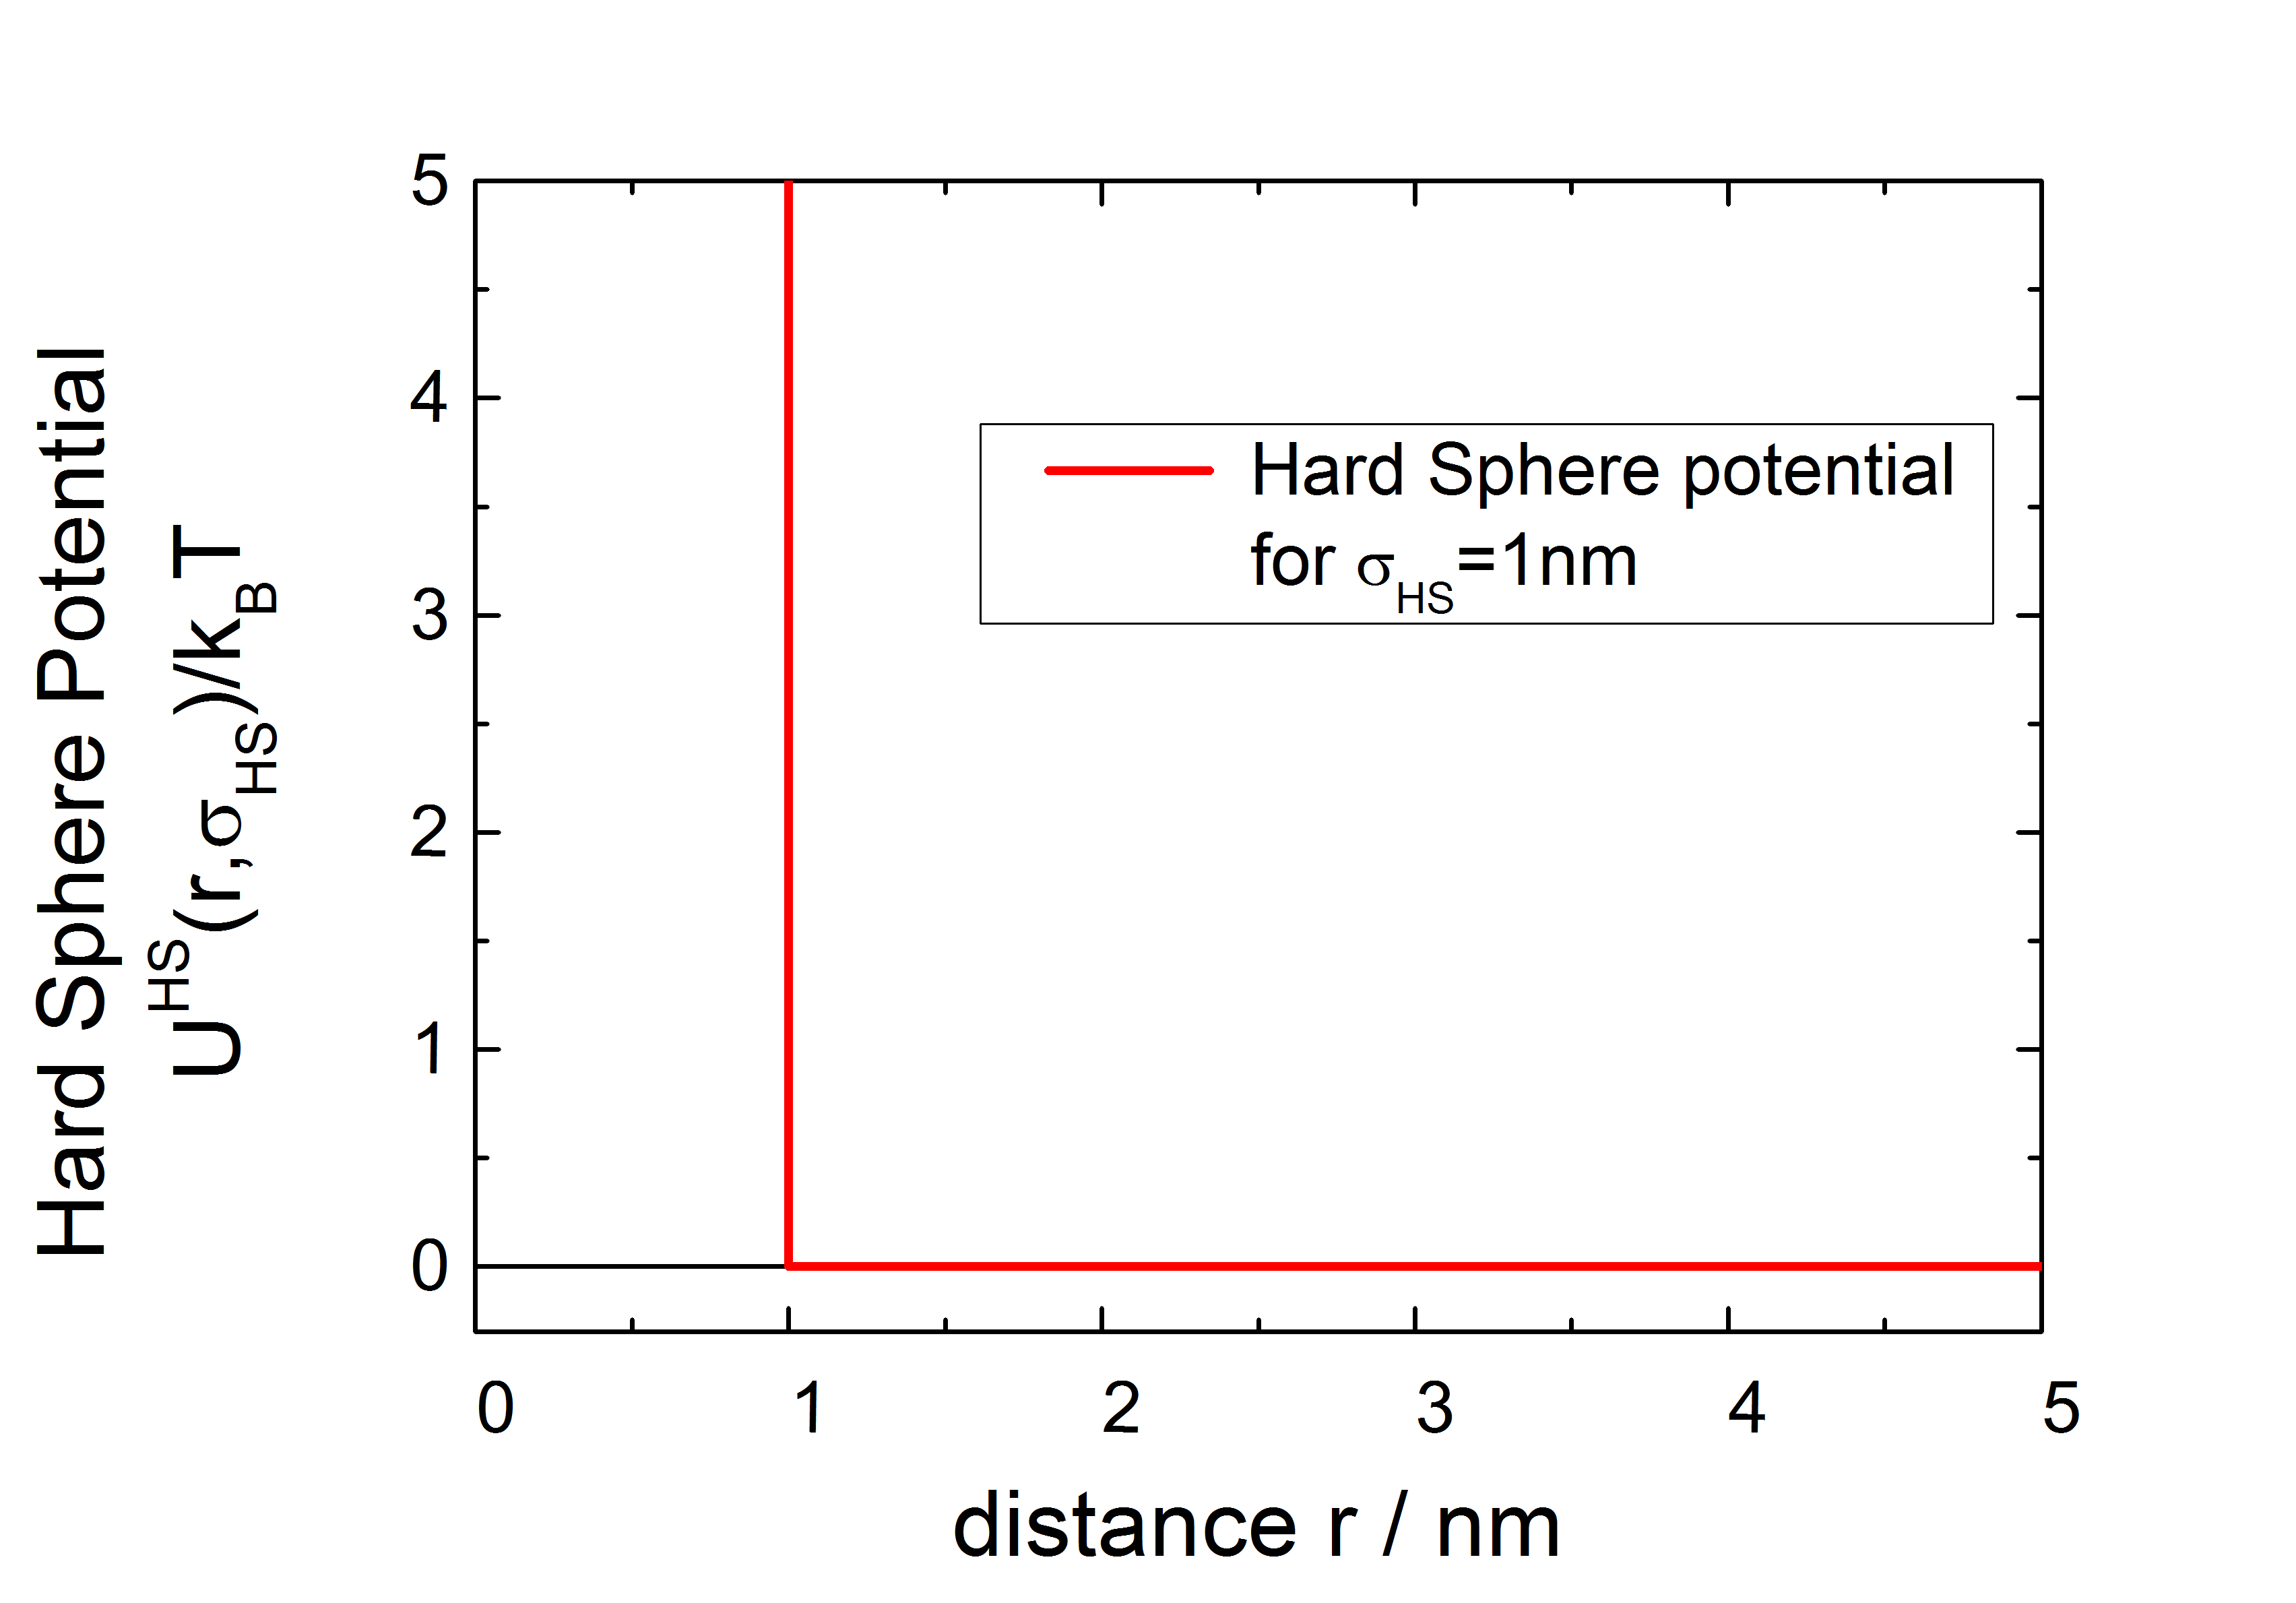
\includegraphics[width=0.45\textwidth,height=0.314\textwidth]{../images/OZsolver/potentials/potUHS.png}}
  \quad
  \subfigure[Mayer-f function of $u^\text{HS}(r,\sigma)$]{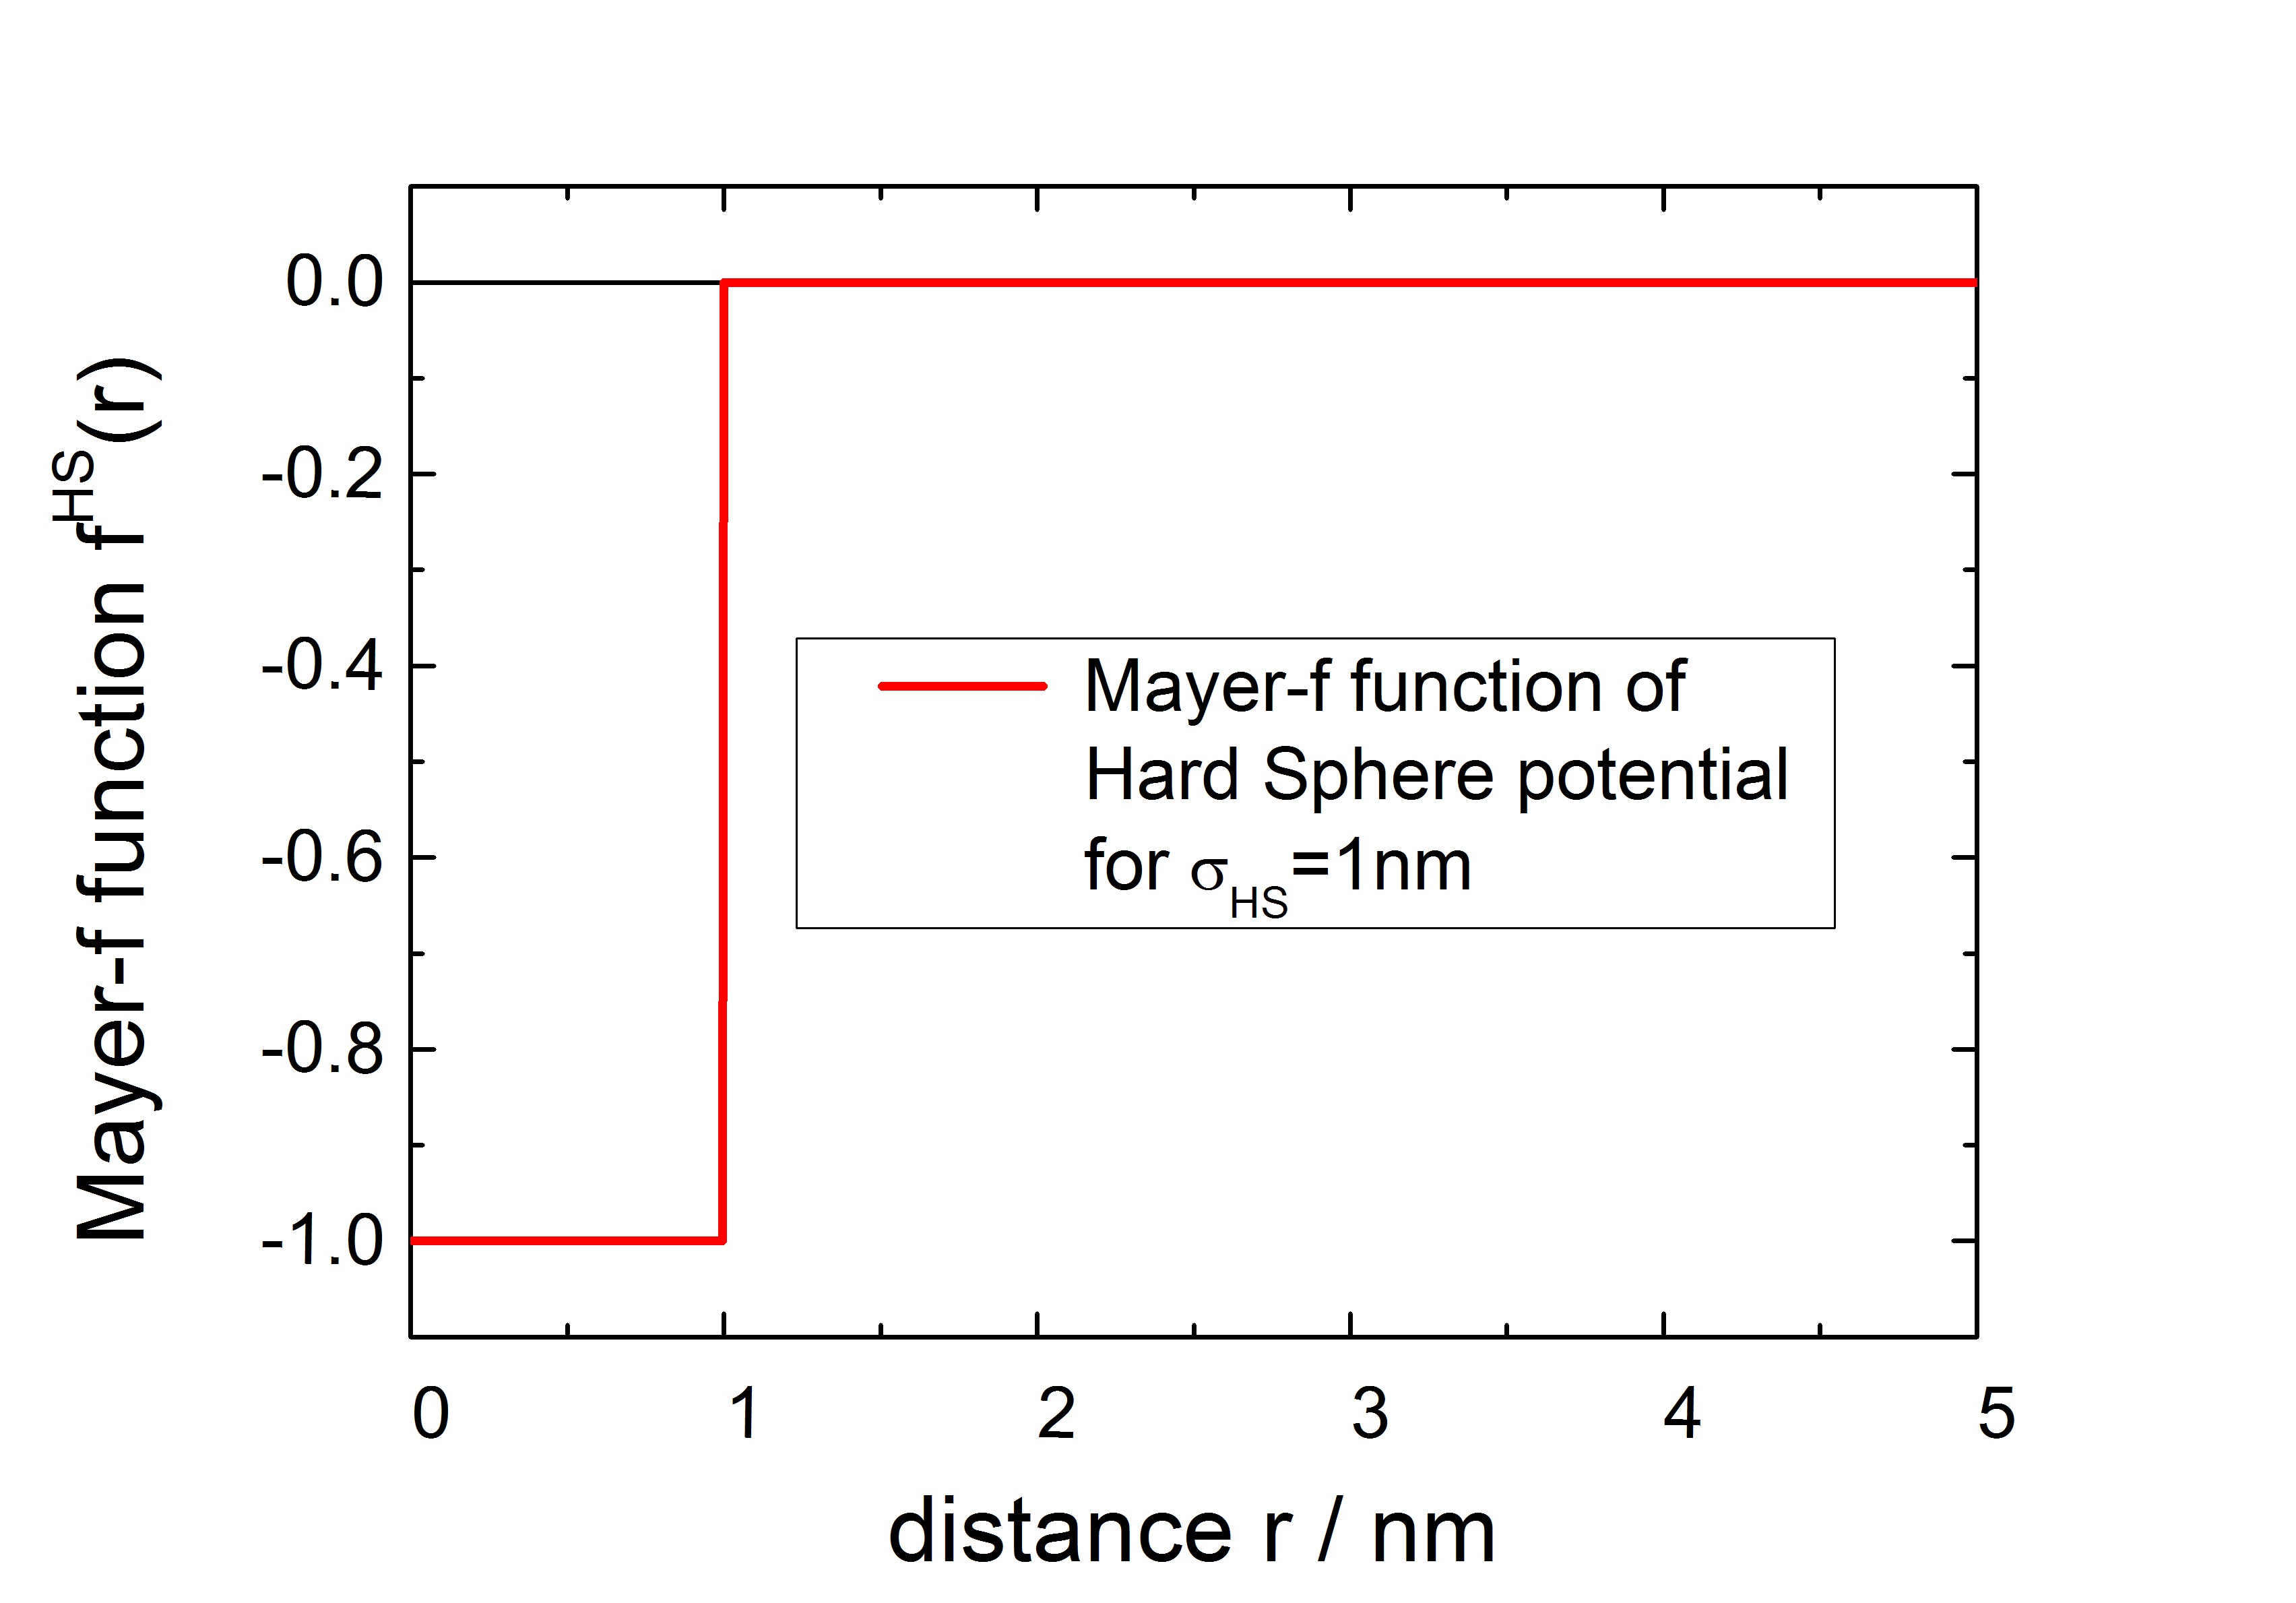
\includegraphics[width=0.45\textwidth,height=0.314\textwidth]{../images/OZsolver/potentials/potfHS.png}}
  \caption{potential $u^\text{HS}(r,\sigma)$ and it's Mayer-f function $\exp(-u^\text{HS}(r,\sigma)/k_BT)-1$}
\end{figure}

 \newpage
\subsection{Sticky Hard Sphere Potential (SHS)}
~\\

The original model of ``adhesive'' or ``sticky'' hard
spheres potential was proposed by Baxter in 1968 \cite{Baxter1968}.
This potential adds to a hard sphere interparticle repulsion an infinitely
strong attraction when molecular surfaces come to contact.
The adhesive surface contribution was defined by a particular
limiting case of a square well tail, in which the well depth goes to
infinity as the width goes to zero, in such a way that the contribution
to the second osmotic virial coefficient $B_2$ remains finite but not
zero (Baxter's ``sticky limit''). More explicitly, in the one-component case,
the square well potential reads as
\begin{align}
u^\text{SHS}(r) &=
\begin{cases}
\infty,   & 0 < r <    \sigma \\
\epsilon, & \sigma \leq r \leq \sigma+\Delta \\
0,        & r > \sigma+\Delta
\end{cases}
\end{align}
with
\begin{align}
\epsilon &= k_\text{B} T \ln\left( \frac{12\tau\Delta}{\sigma+\Delta} \right)
\end{align}
The hight of the square well $\epsilon$ is positive for $\tau>(\sigma+\Delta)/(12\Delta)$.
Therefore the splitting in attractive and repulsive potential is done as
\begin{align}
u^\text{SHS}_\text{A}(r) &=
\begin{cases}
\epsilon & \tau < \frac{\sigma+\Delta}{12\Delta} \wedge r \leq \sigma+\Delta \\
0        & \mbox{otherwise}
\end{cases}
\\
u^\text{SHS}_\text{R}(r) &=
\begin{cases}
\infty & r < \sigma \\
\epsilon  & \tau > \frac{\sigma+\Delta}{12\Delta} \wedge \sigma \leq r \leq \sigma+\Delta \\
0         & \tau < \frac{\sigma+\Delta}{12\Delta} \wedge \sigma \leq r \leq \sigma+\Delta \\
0         & \mbox{otherwise}
\end{cases}
\end{align}
The partitioning in reference and perturbation is done by
\begin{align}
u^\text{SHS}_\text{ref}(r) &=
\begin{cases}
\infty & r < \sigma \\
0        & \mbox{otherwise}
\end{cases}
\\
u^\text{SHS}_\text{pert}(r) &=
\begin{cases}
\epsilon  & r <= \sigma +\Delta\\
0         & \mbox{otherwise}
\end{cases}
\end{align}
A partitioning in long range and short range is not done. The long range potential
is set to be always $u^\text{SHS}_\text{LR}(r) \equiv 0$, so that
$u^\text{SHS}_\text{SR}(r)= u^\text{SHS}(r)$.

\begin{figure}[htb]
\centering
  \subfigure[Sticky Hard Sphere potential $u^\text{SHS}(r,\sigma)$]{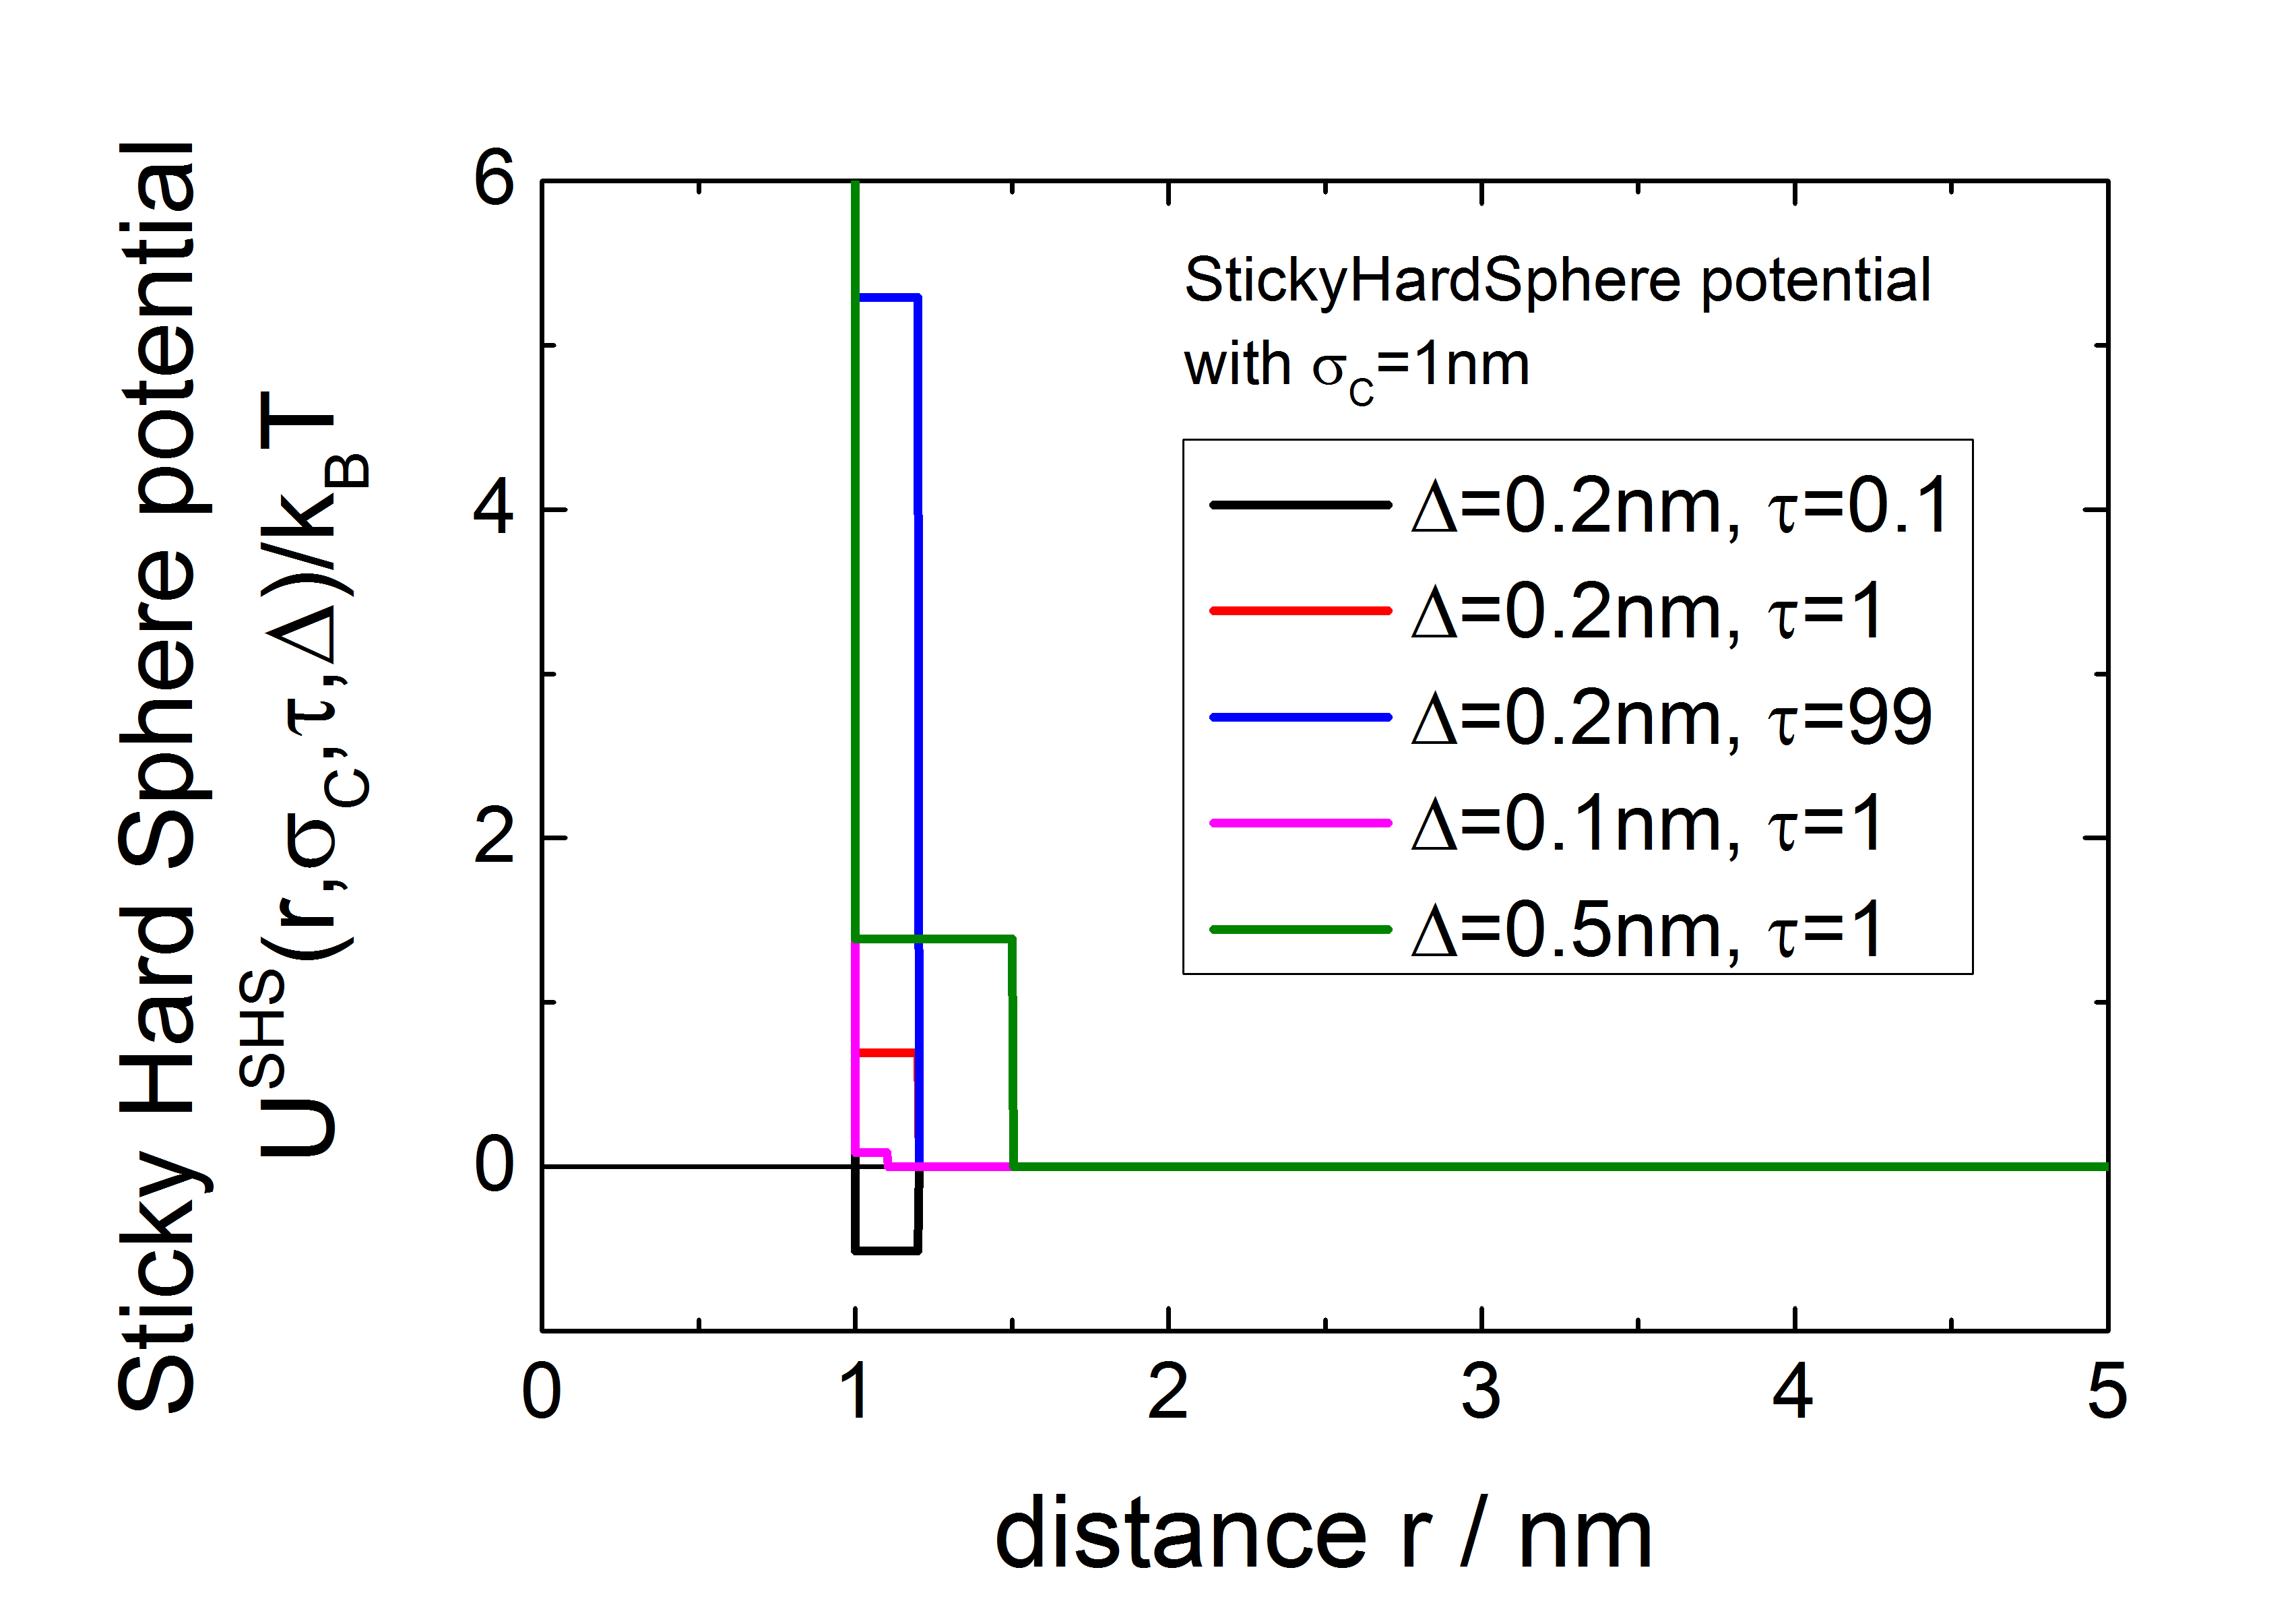
\includegraphics[width=0.45\textwidth,height=0.314\textwidth]{../images/OZsolver/potentials/potUSHS.png}}
  \quad
  \subfigure[Mayer-f function of $u^\text{SHS}(r,\sigma)$]{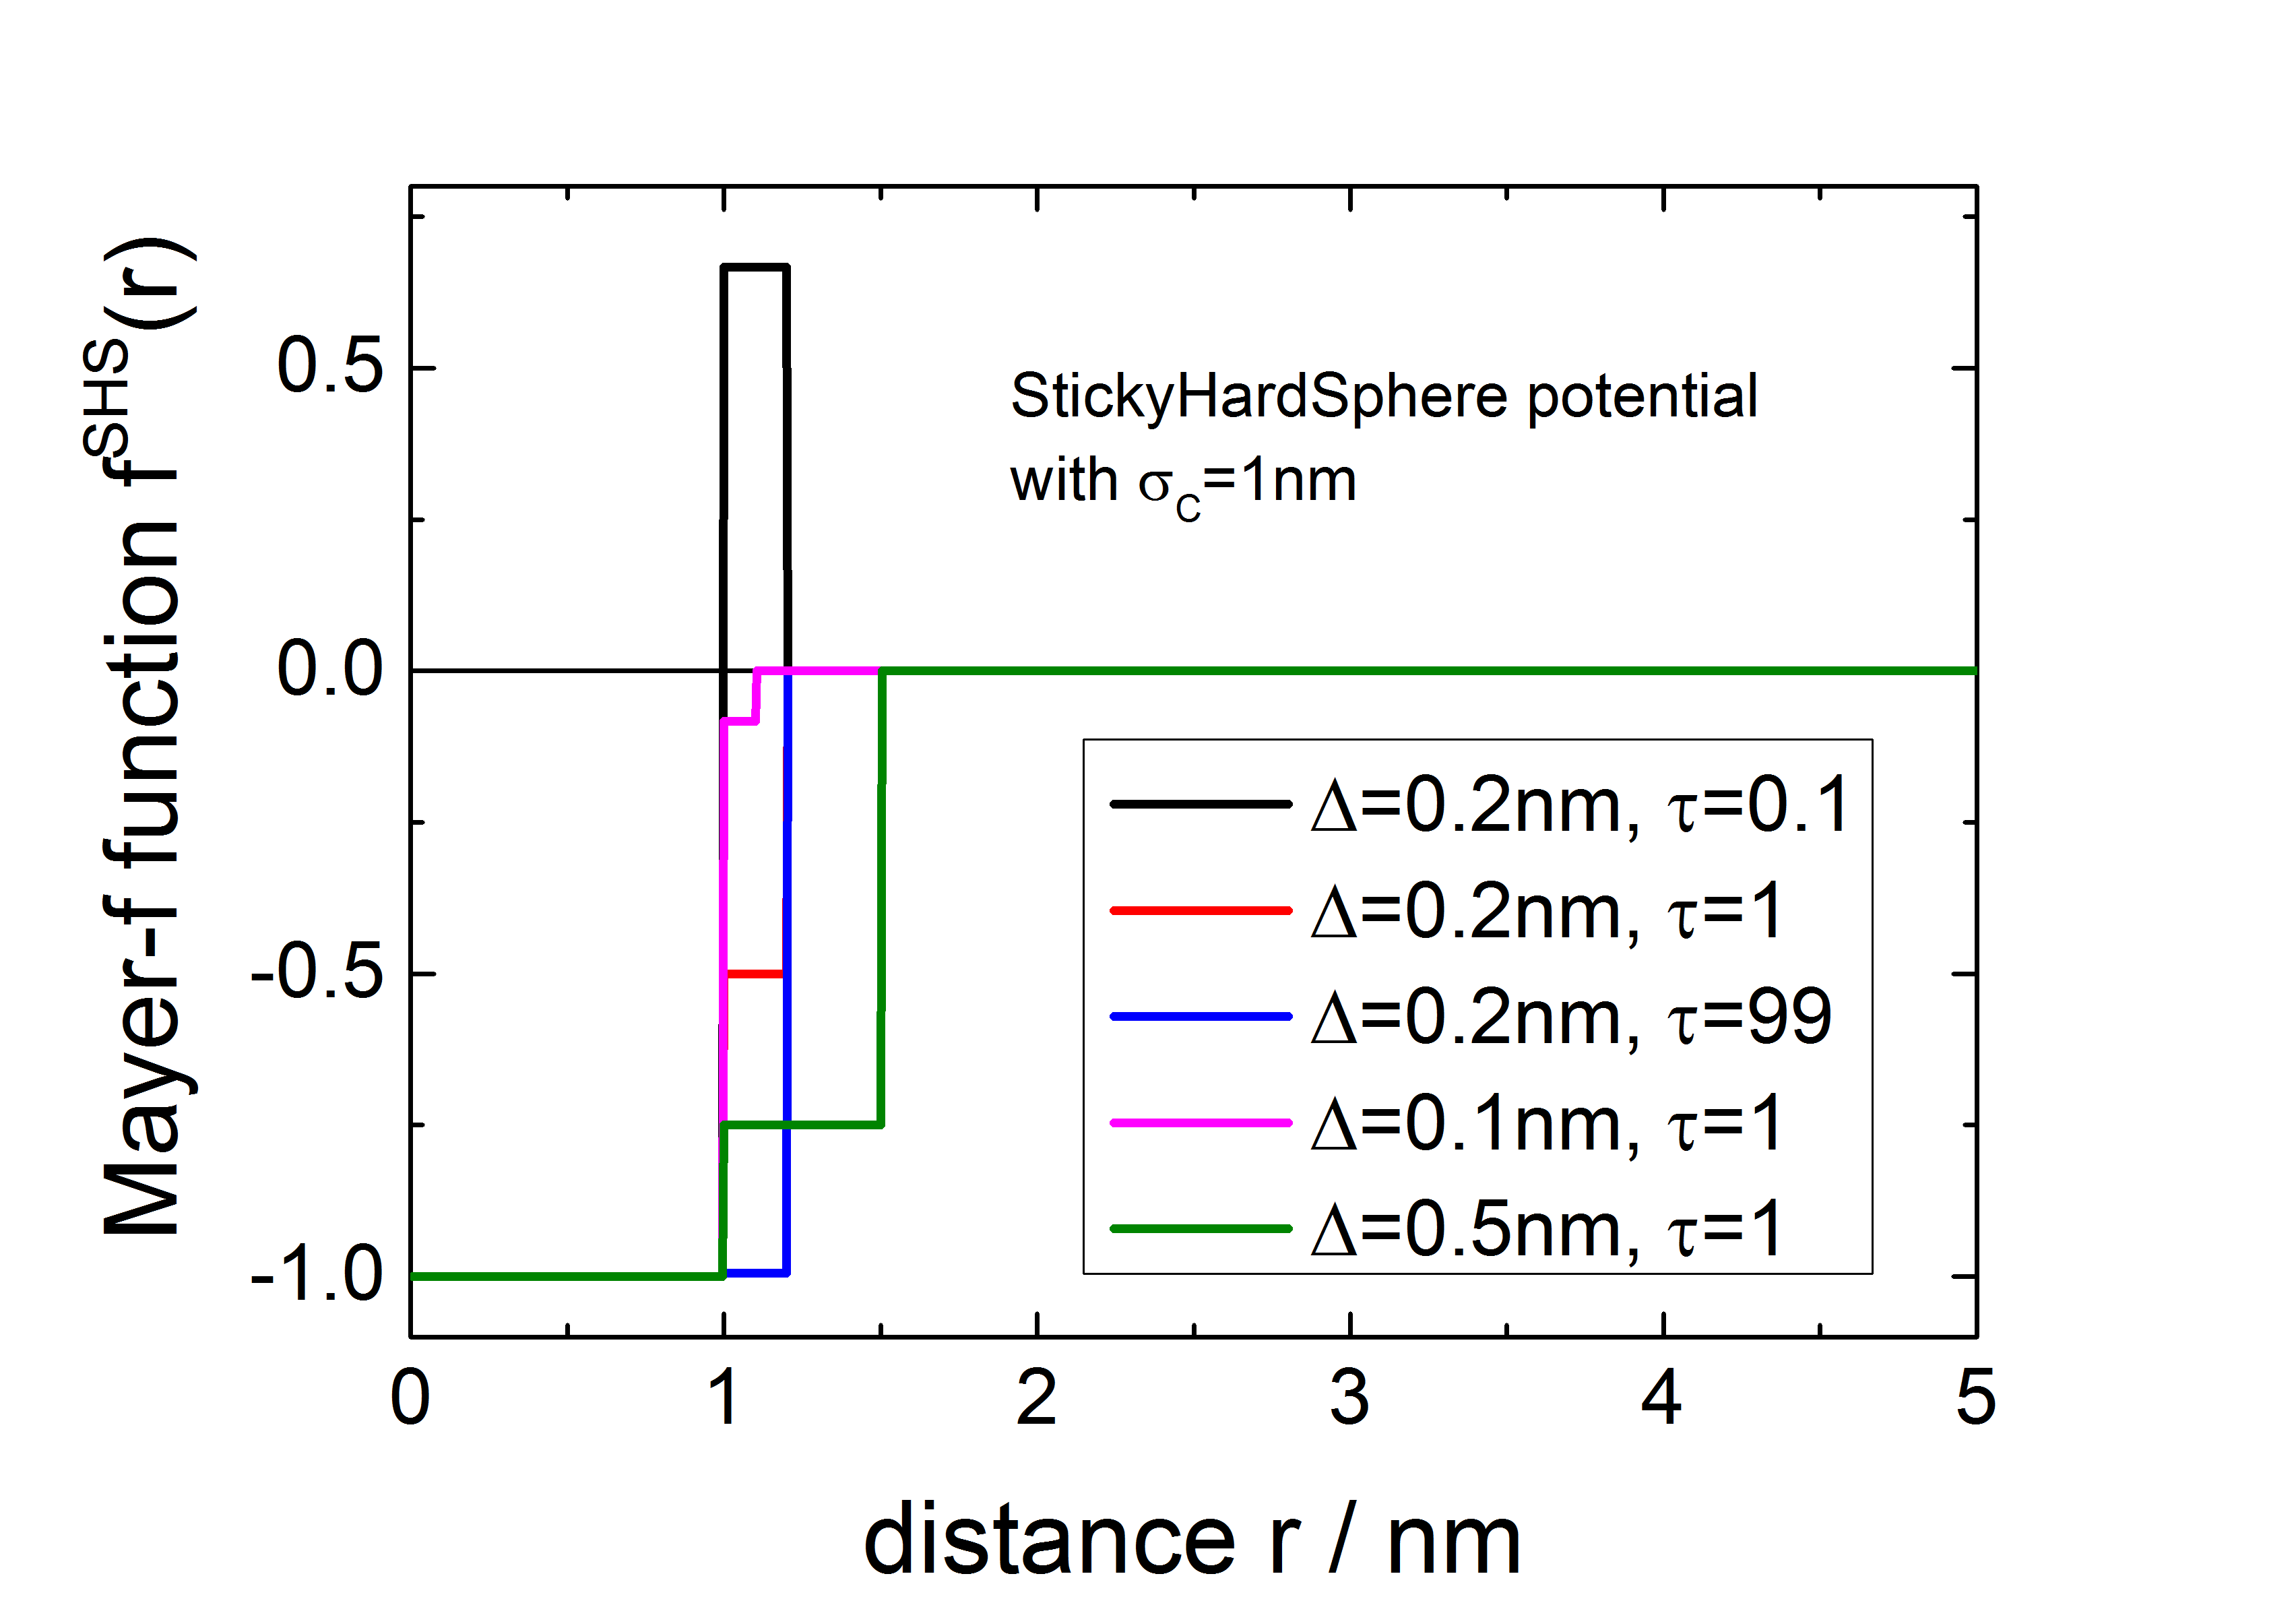
\includegraphics[width=0.45\textwidth,height=0.314\textwidth]{../images/OZsolver/potentials/potfSHS.png}}
  \caption{potential $u^\text{SHS}(r,\sigma)$ and it's Mayer-f function $\exp(-u^\text{SHS}(r,\sigma)/k_BT)-1$}
\end{figure}

% \vphantom{.}~\\
\clearpage
\subsection{Soft Sphere Potential}
~\\

The soft sphere potential is define as
\begin{align}
u^\text{SSP}(r,\sigma,\epsilon) &=
k_\text{B} T \epsilon \left(\frac{\sigma}{r}\right)^n
\end{align}
$\sigma$ is the nominal particle diameter, $\epsilon$ establishes the
energy scale, and $n$ controls the stiffness of the potential (the
softness is $1/n$). Indeed for microgel particles this potential
form has been used to interpret experimentally measured
physical properties. $n\rightarrow\infty$ is the hard sphere limit, and this
and intermediate $n$ values (particularly $n=12$) have been
studied many times in the literature. For $n\leq 3$
this potential does not lead to a thermodynamically stable
system as the volume integral of the potential diverges.


%\begin{align}
%u^\text{SSM}(r,\sigma,\epsilon) &=
%\begin{cases}
%k_\text{B} T \epsilon \left(1-\frac{r}{\sigma}\right)^2   & \mbox{if } r \leq \sigma \\
%0                       & \mbox{if } r >    \sigma
%\end{cases}
%\end{align}

\begin{figure}[htb]
\centering
  \subfigure[Soft Sphere Potential $u^\text{SSP}(r,\sigma,\ldots)$]{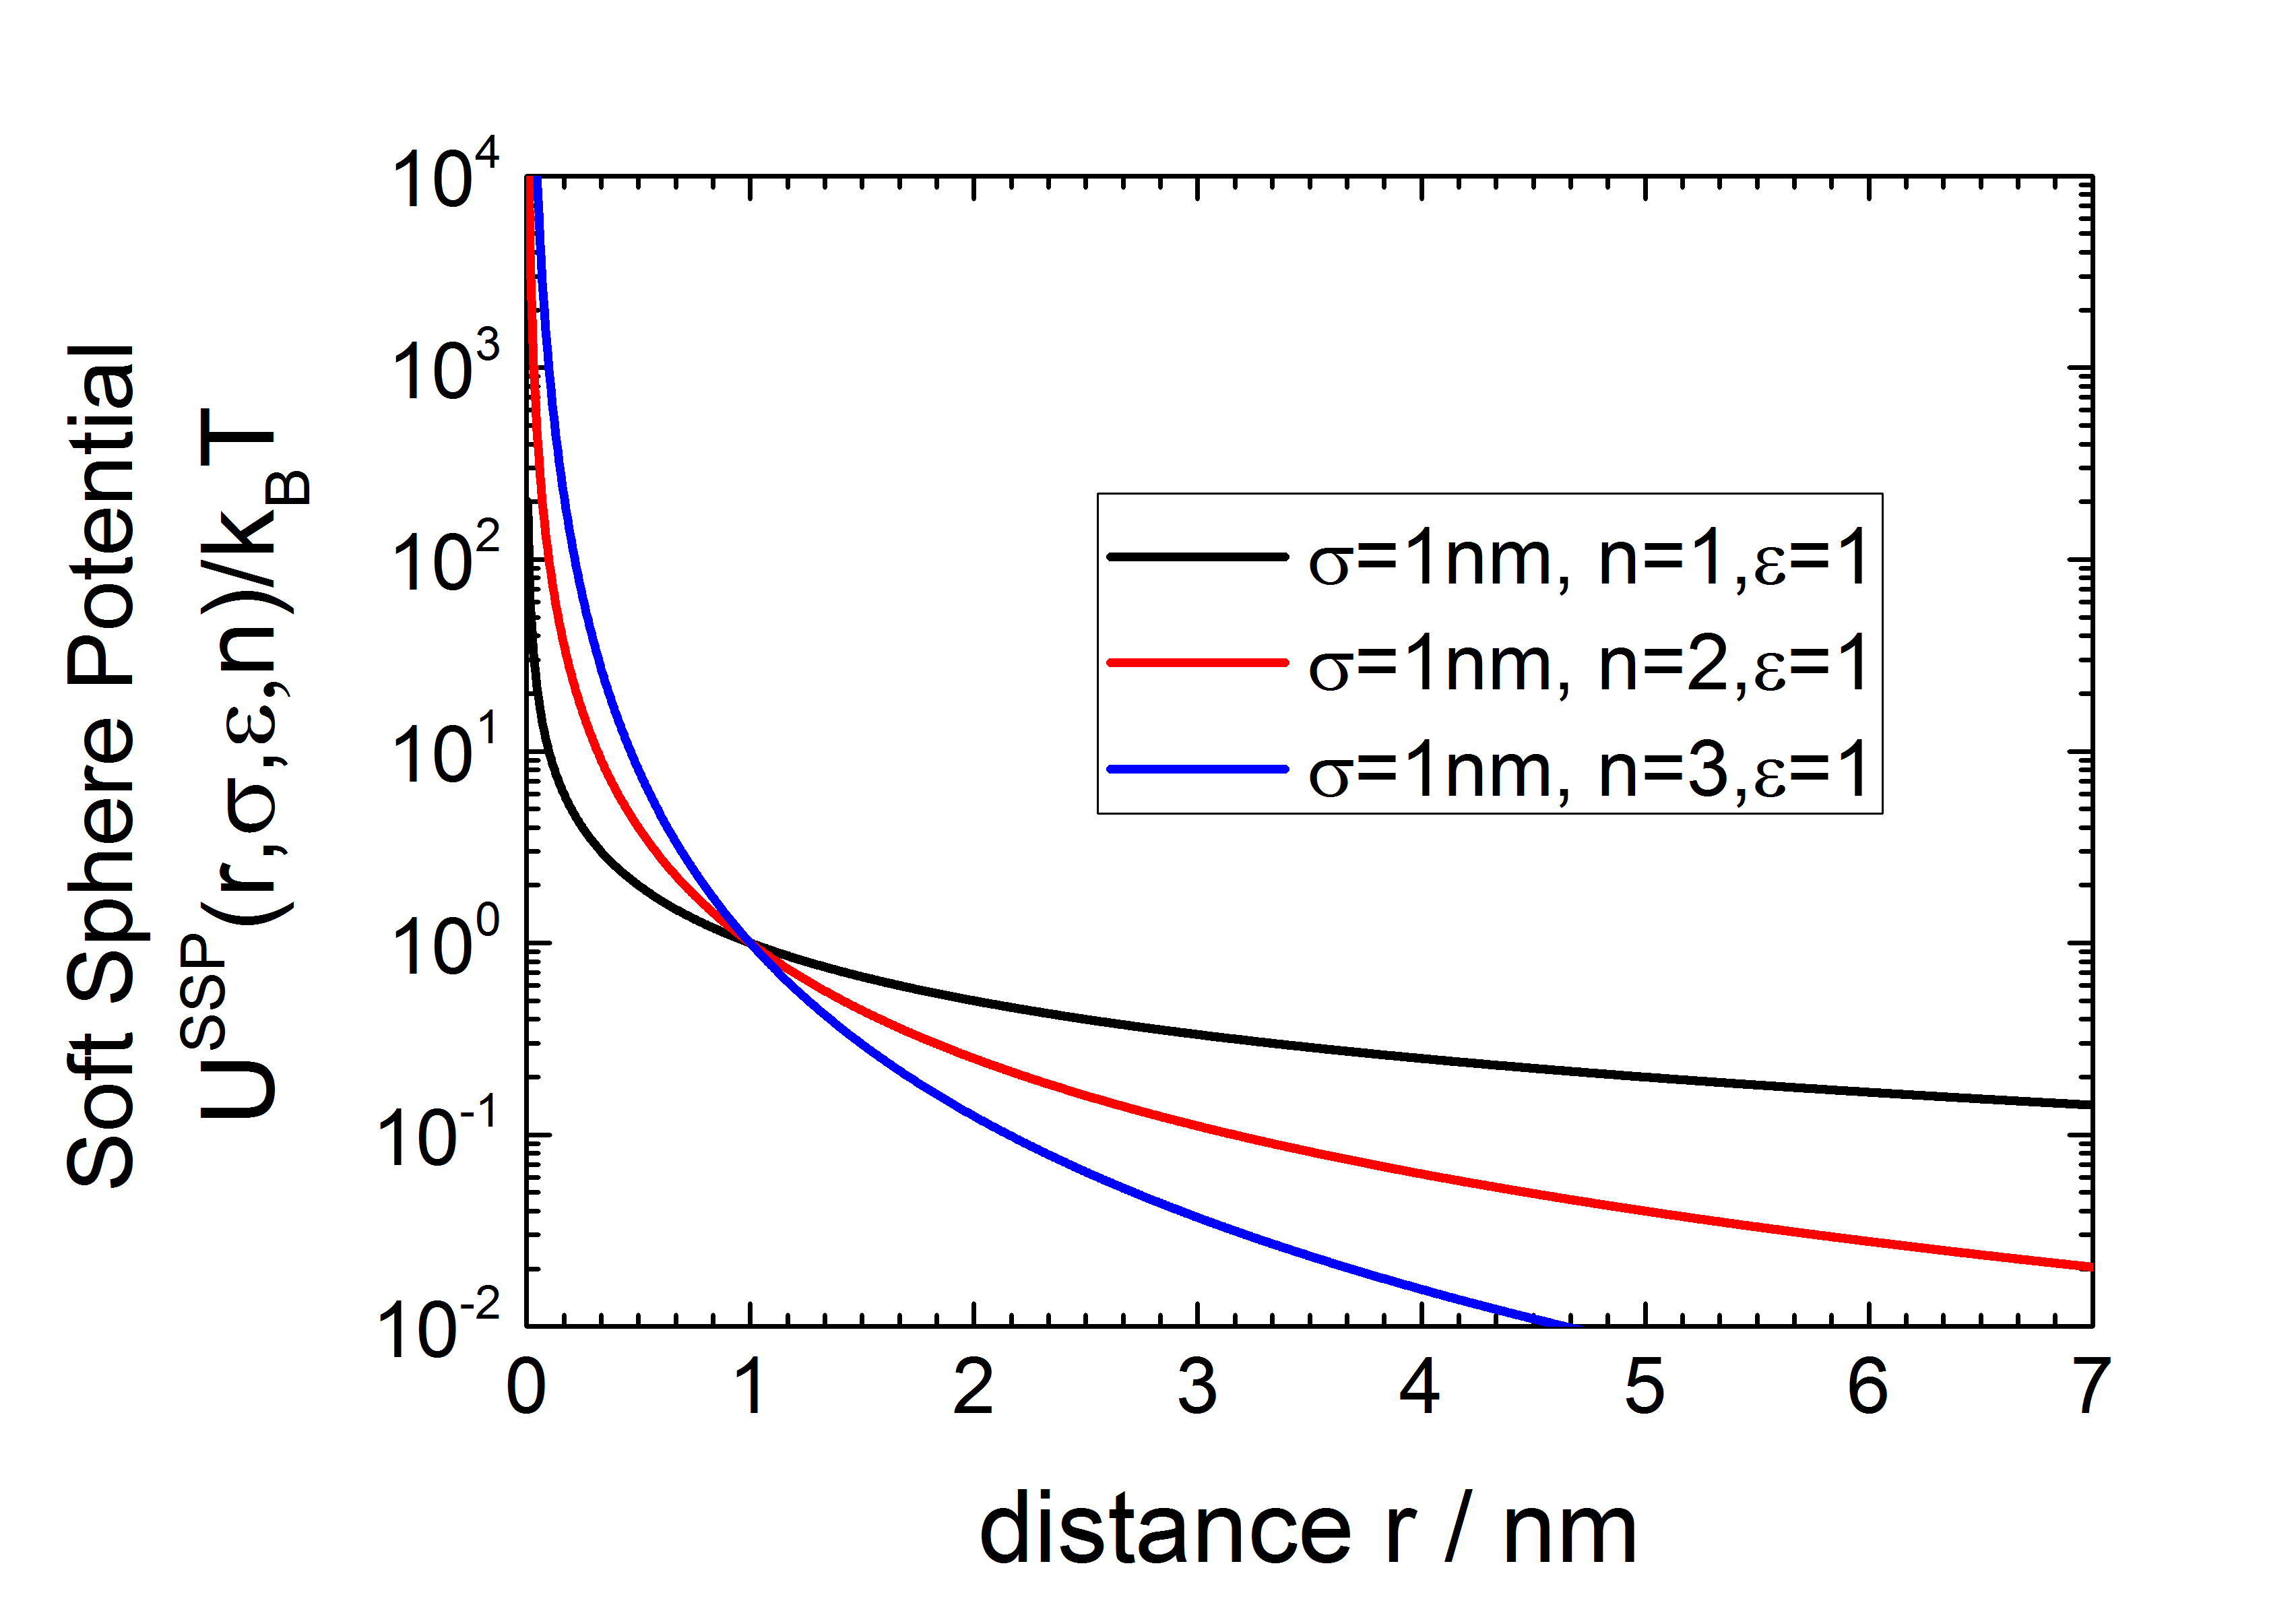
\includegraphics[width=0.45\textwidth,height=0.314\textwidth]{../images/OZsolver/potentials/potUSoftSphere.png}}
  \quad
  \subfigure[Mayer-f function of $u^\text{SSP}(r,\sigma,\ldots)$]{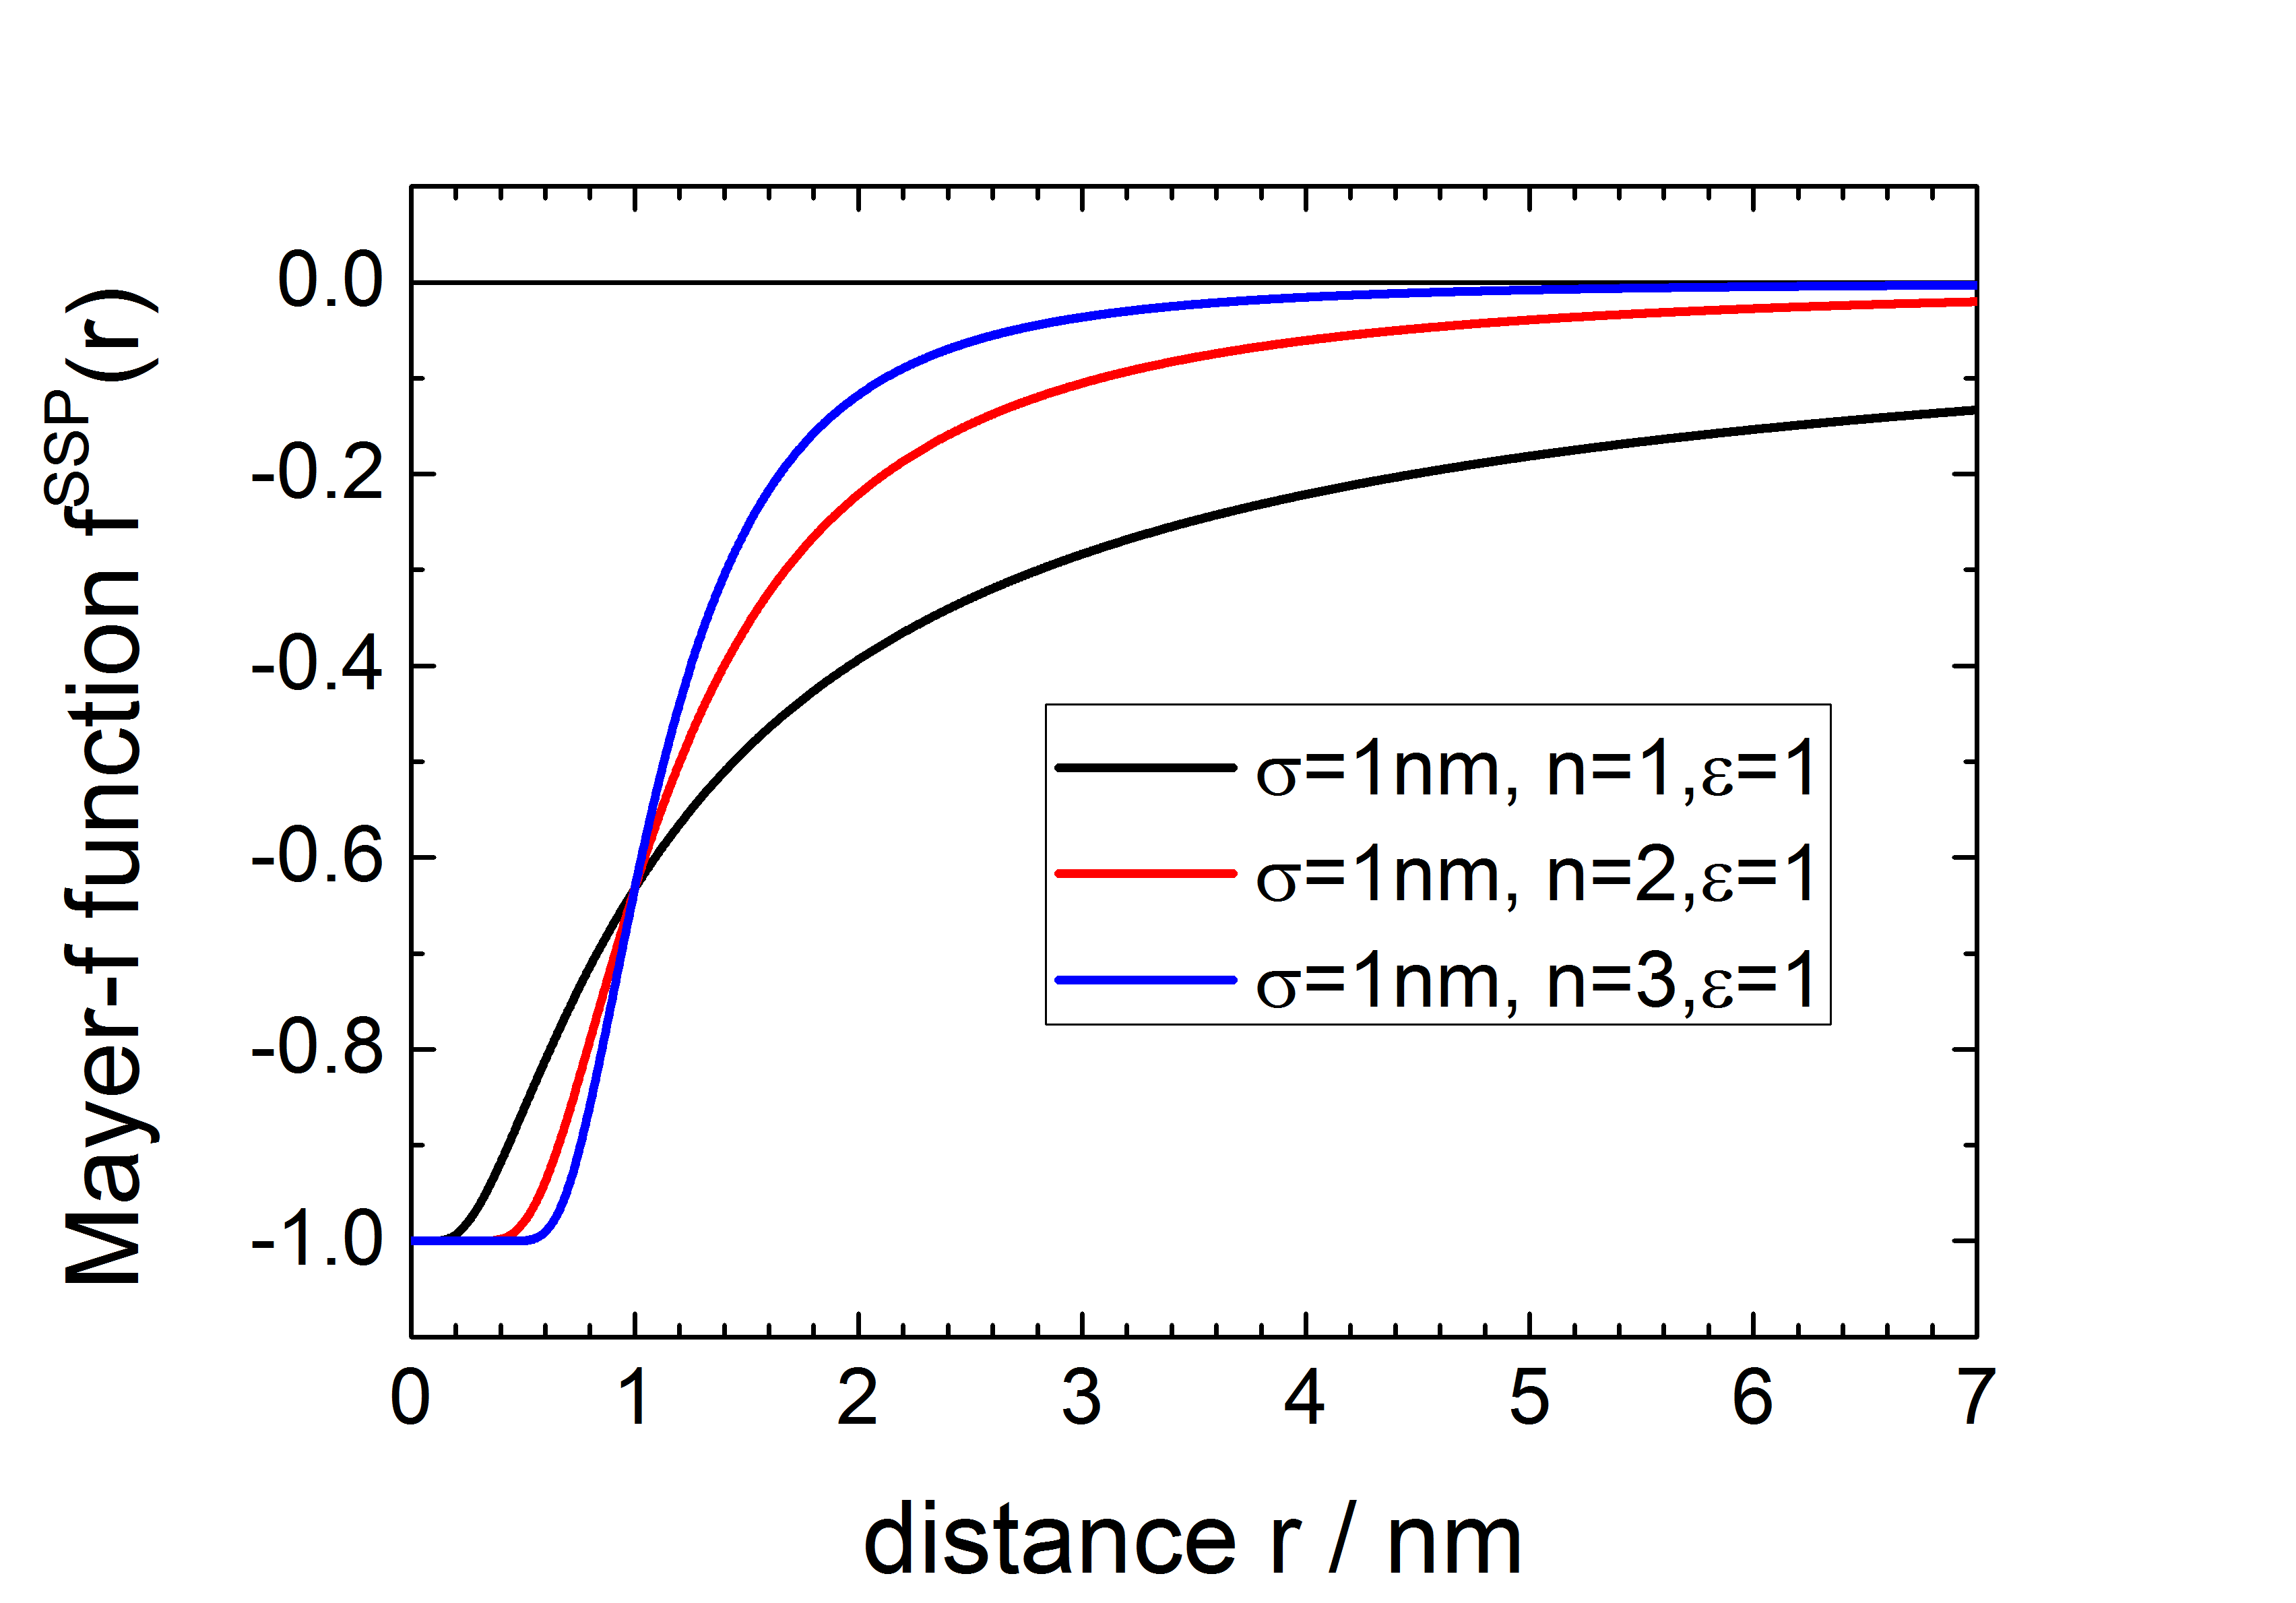
\includegraphics[width=0.45\textwidth,height=0.314\textwidth]{../images/OZsolver/potentials/potfSoftSphere.png}}
  \caption{potential $u^\text{SSP}(r,\sigma,\ldots)$ and it's Mayer-f function $\exp(-u^\text{SSP}(r,\sigma,\ldots)/k_BT)-1$}
\end{figure}

% \vphantom{.}~\\
\newpage
\subsection{Penetrable Sphere Model}
~\\

The penetrable sphere model was used by Marquest and
Witten \cite{Marquest1989} who suggested it as a prototype for the interaction between micelles in a solvent.
The potential is defined as \cite{Marquest1989,Viererblova2010}
\begin{align}
u^\text{PSM}(r,\sigma,\epsilon) &=
\begin{cases}
k_\text{B} T \epsilon   & \mbox{for } r \leq \sigma \\
0                       & \mbox{for } r >    \sigma
\end{cases}
\end{align}

\begin{figure}[htb]
\centering
  \subfigure[Potential of the Penetrable Sphere Model (PSM) $u^\text{PSM}(r,\sigma,\ldots)$]{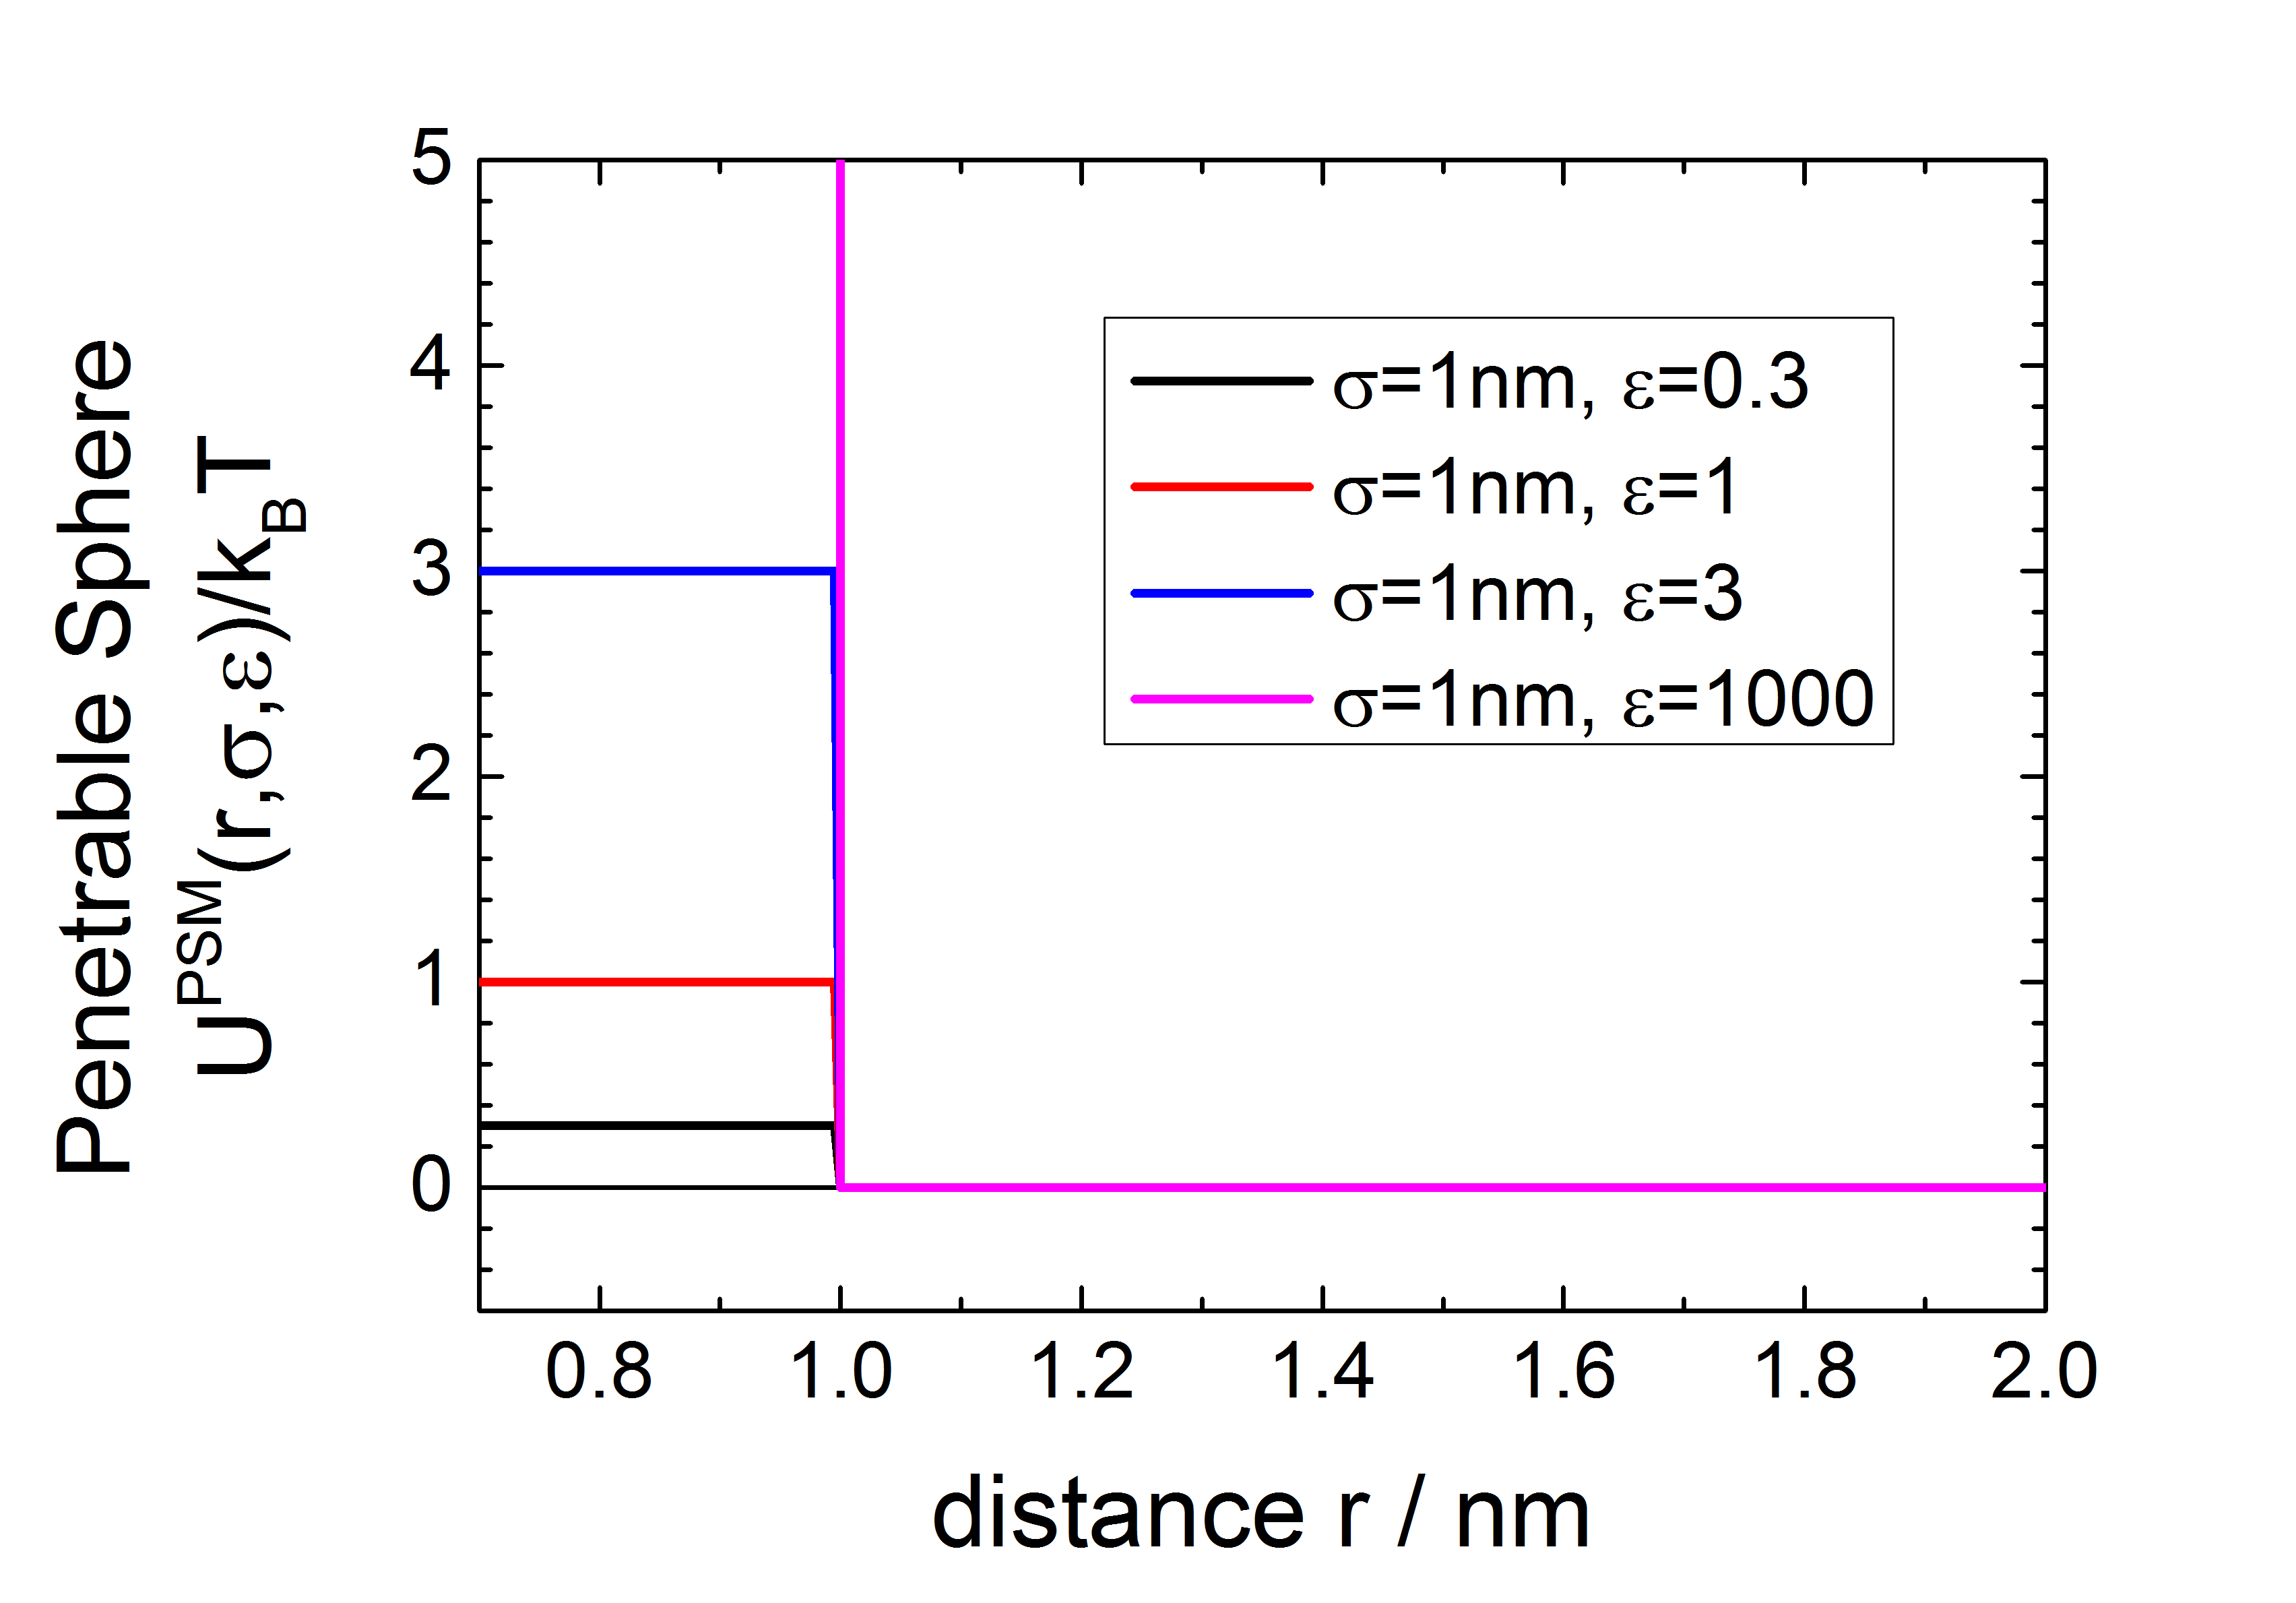
\includegraphics[width=0.45\textwidth,height=0.314\textwidth]{../images/OZsolver/potentials/potUPenetrableSphere.png}}
  \quad
  \subfigure[Mayer-f function of $u^\text{PSM}(r,\sigma,\ldots)$]{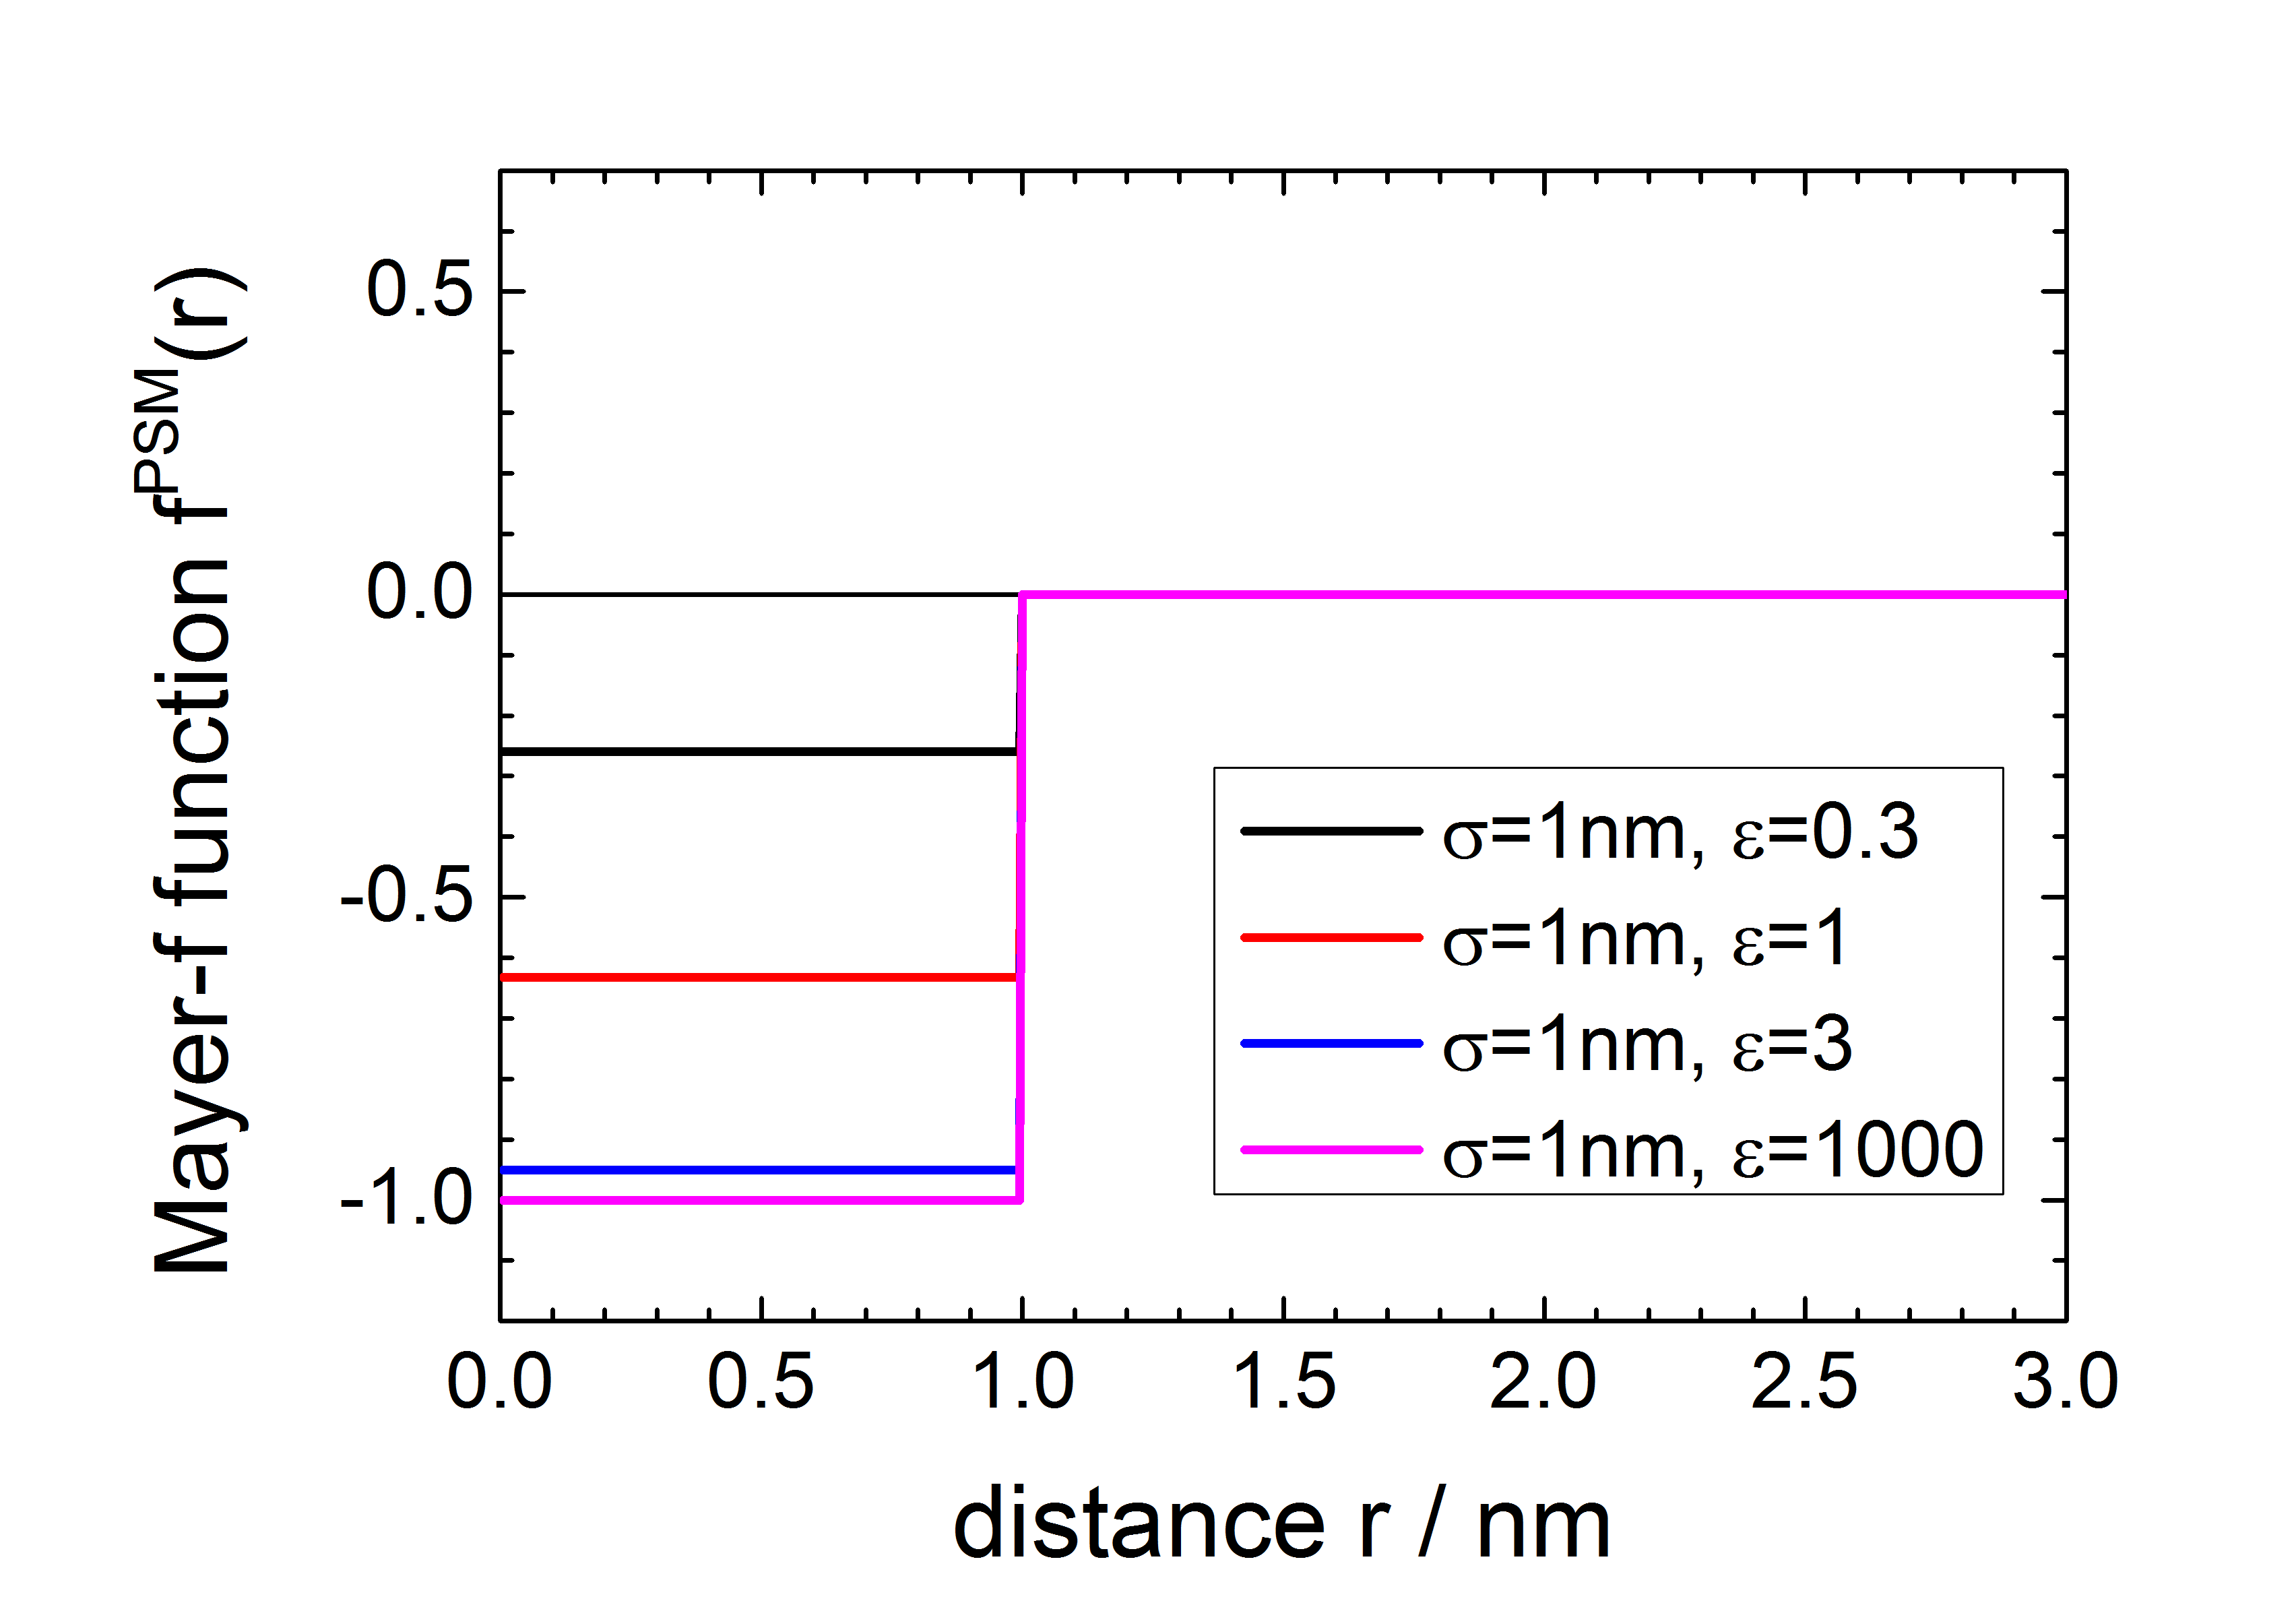
\includegraphics[width=0.45\textwidth,height=0.314\textwidth]{../images/OZsolver/potentials/potfPenetrableSphere.png}}
  \caption{potential $u^\text{PSM}(r,\sigma,\ldots)$ and it's Mayer-f function $\exp(-u^\text{PSM}(r,\sigma,\ldots)/k_BT)-1$}
\end{figure}

% \vphantom{.}~\\
\newpage
\subsection{Generalized Gaussian Core Model Potential - GGCM-n Potential}
~\\

The effective interaction between the centers of mass of two polymer chains
in an athermal solvent can be described in very good approximation
by an interaction of a Gaussian form
$u^\text{GCM}(r)= k_\text{B} T \epsilon \exp\left(-\left(r/\sigma\right)^2\right)$.
A generalisation of this form has been discussed in \cite{Mladek2005,Louis2000} and
has the form
\begin{align}
u^\text{GGCM-n}(r)&=
k_\text{B} T \epsilon \exp\left(-\alpha\left(\frac{r}{\sigma}\right)^n\right)
\end{align}

\begin{figure}[htb]
\centering
  \subfigure[Potential of the Generalises Gaussian Code Model (GGCM-n) $u^\text{GGCM-n}(r,\sigma,\ldots)$]{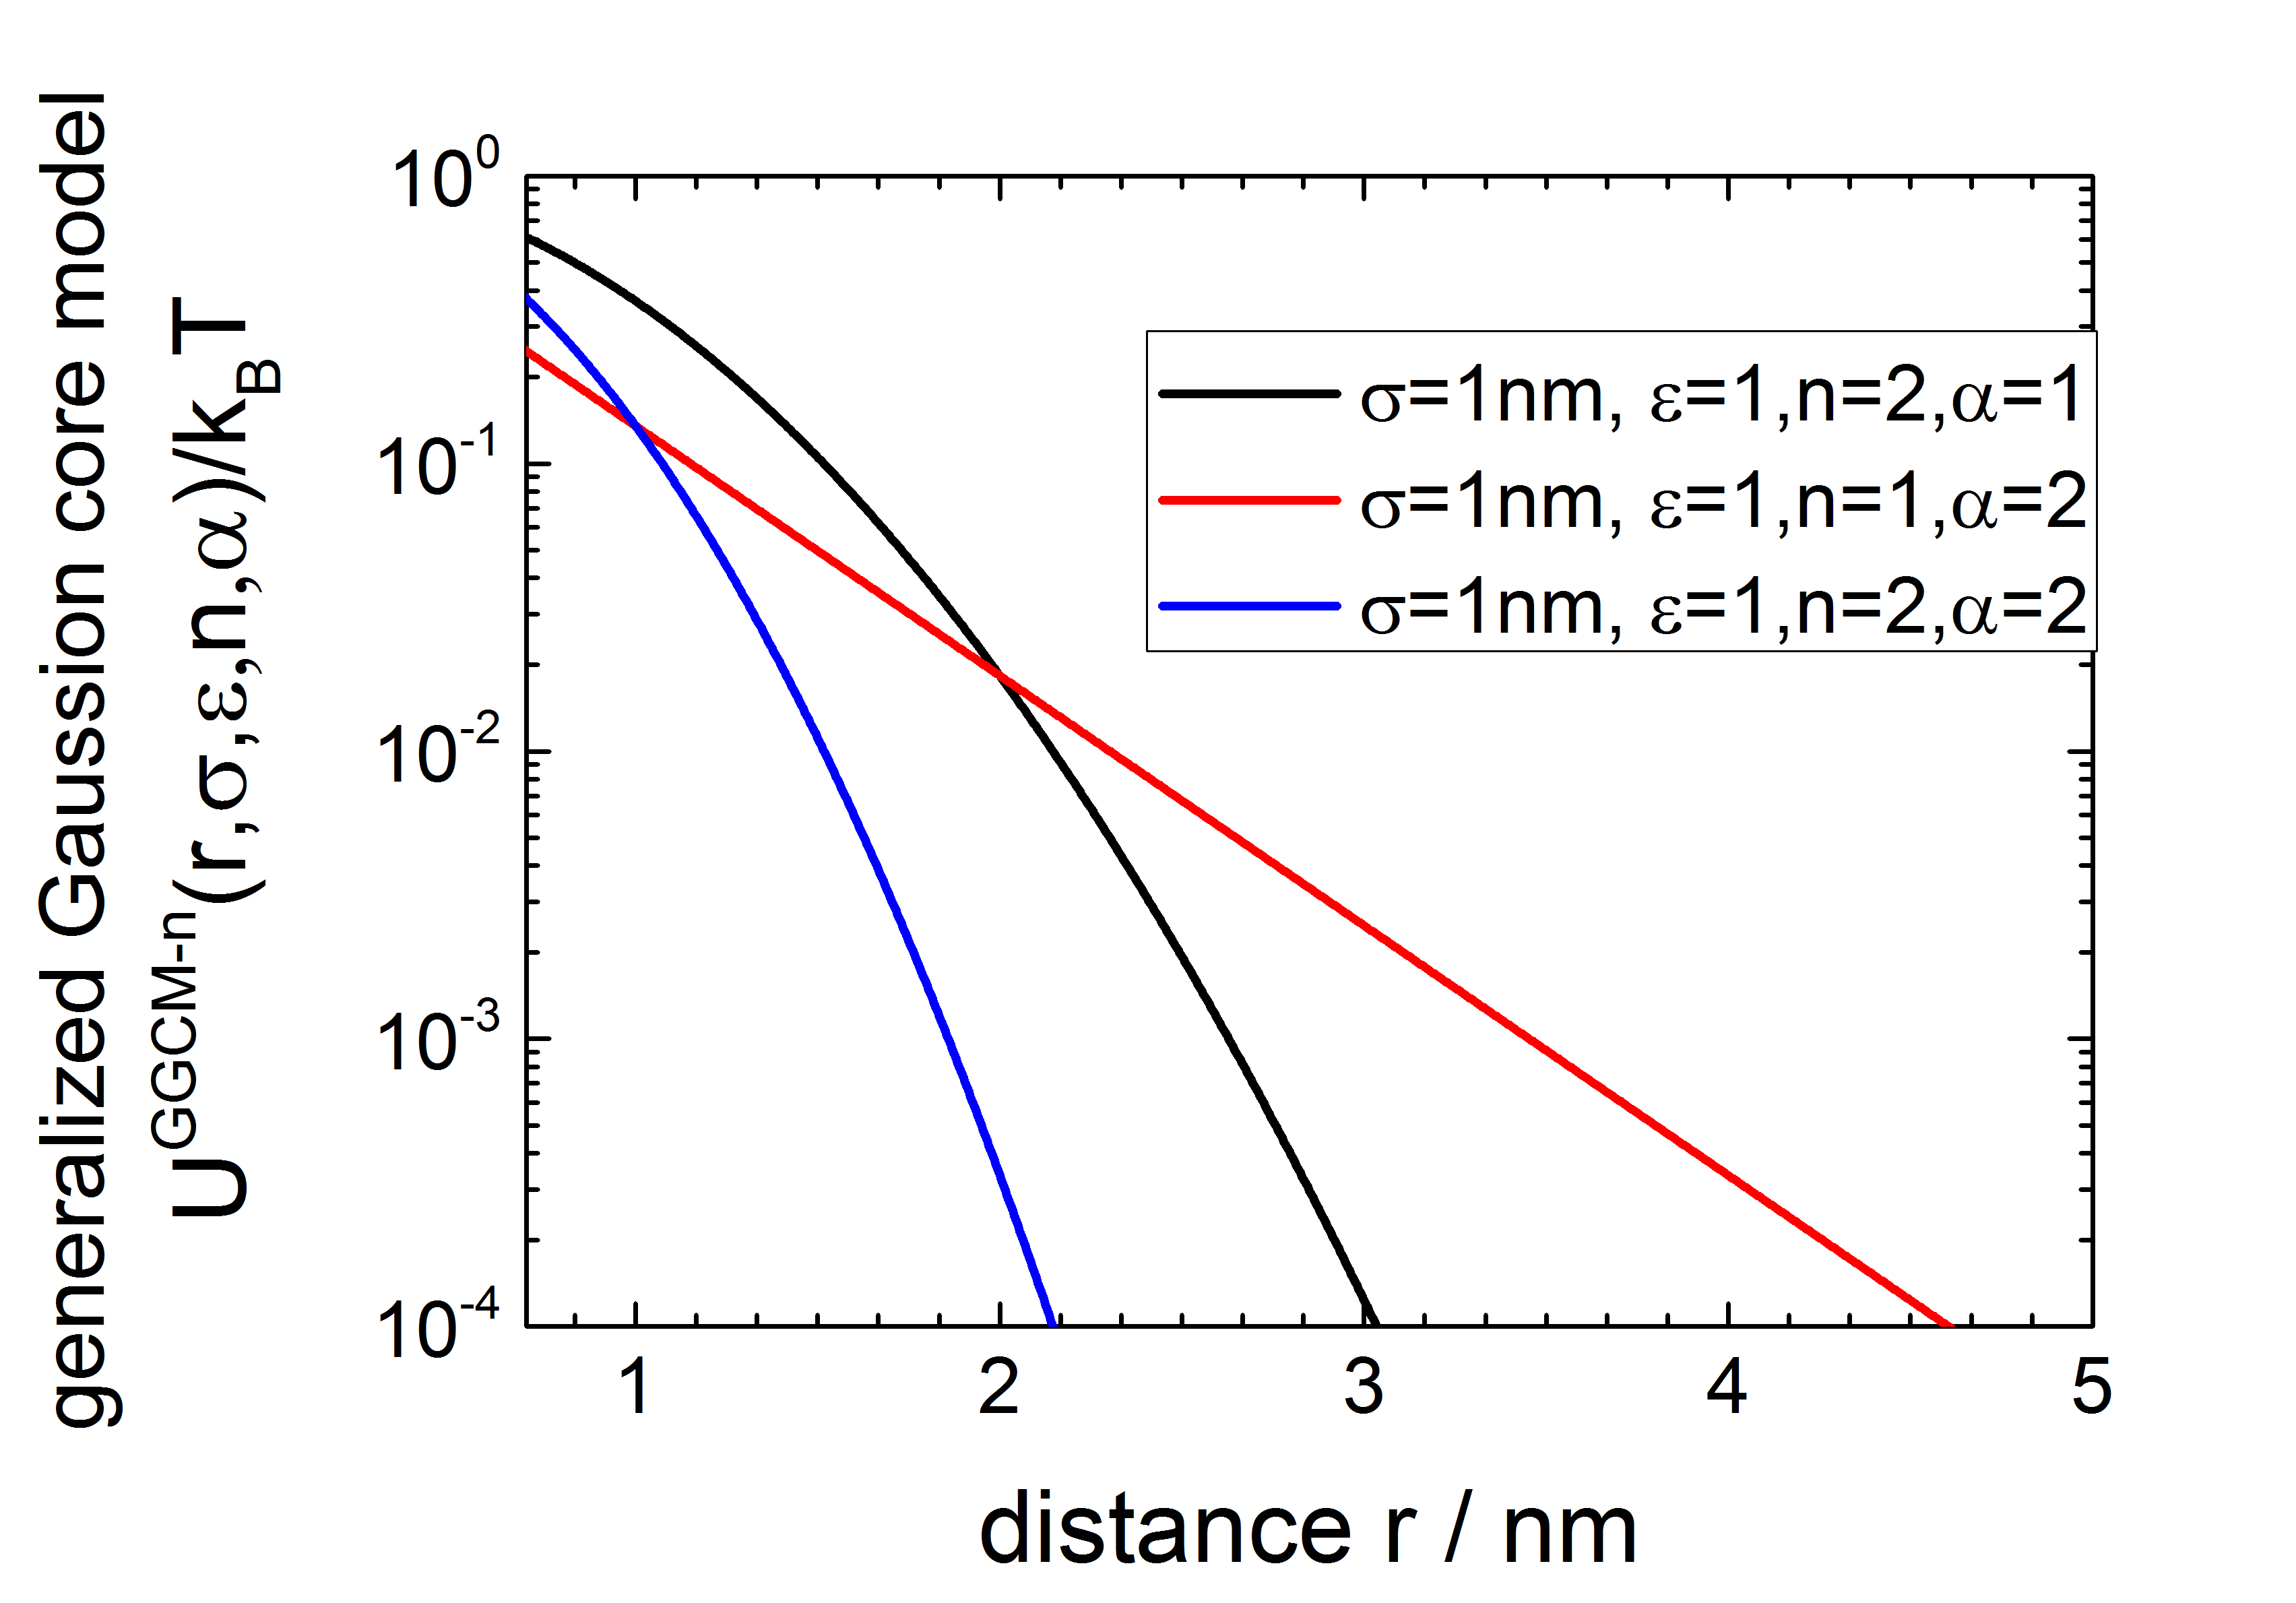
\includegraphics[width=0.45\textwidth,height=0.314\textwidth]{../images/OZsolver/potentials/potUGGCM-n.png}}
  \quad
  \subfigure[Mayer-f function of $u^\text{GGCM-n}(r,\sigma,\ldots)$]{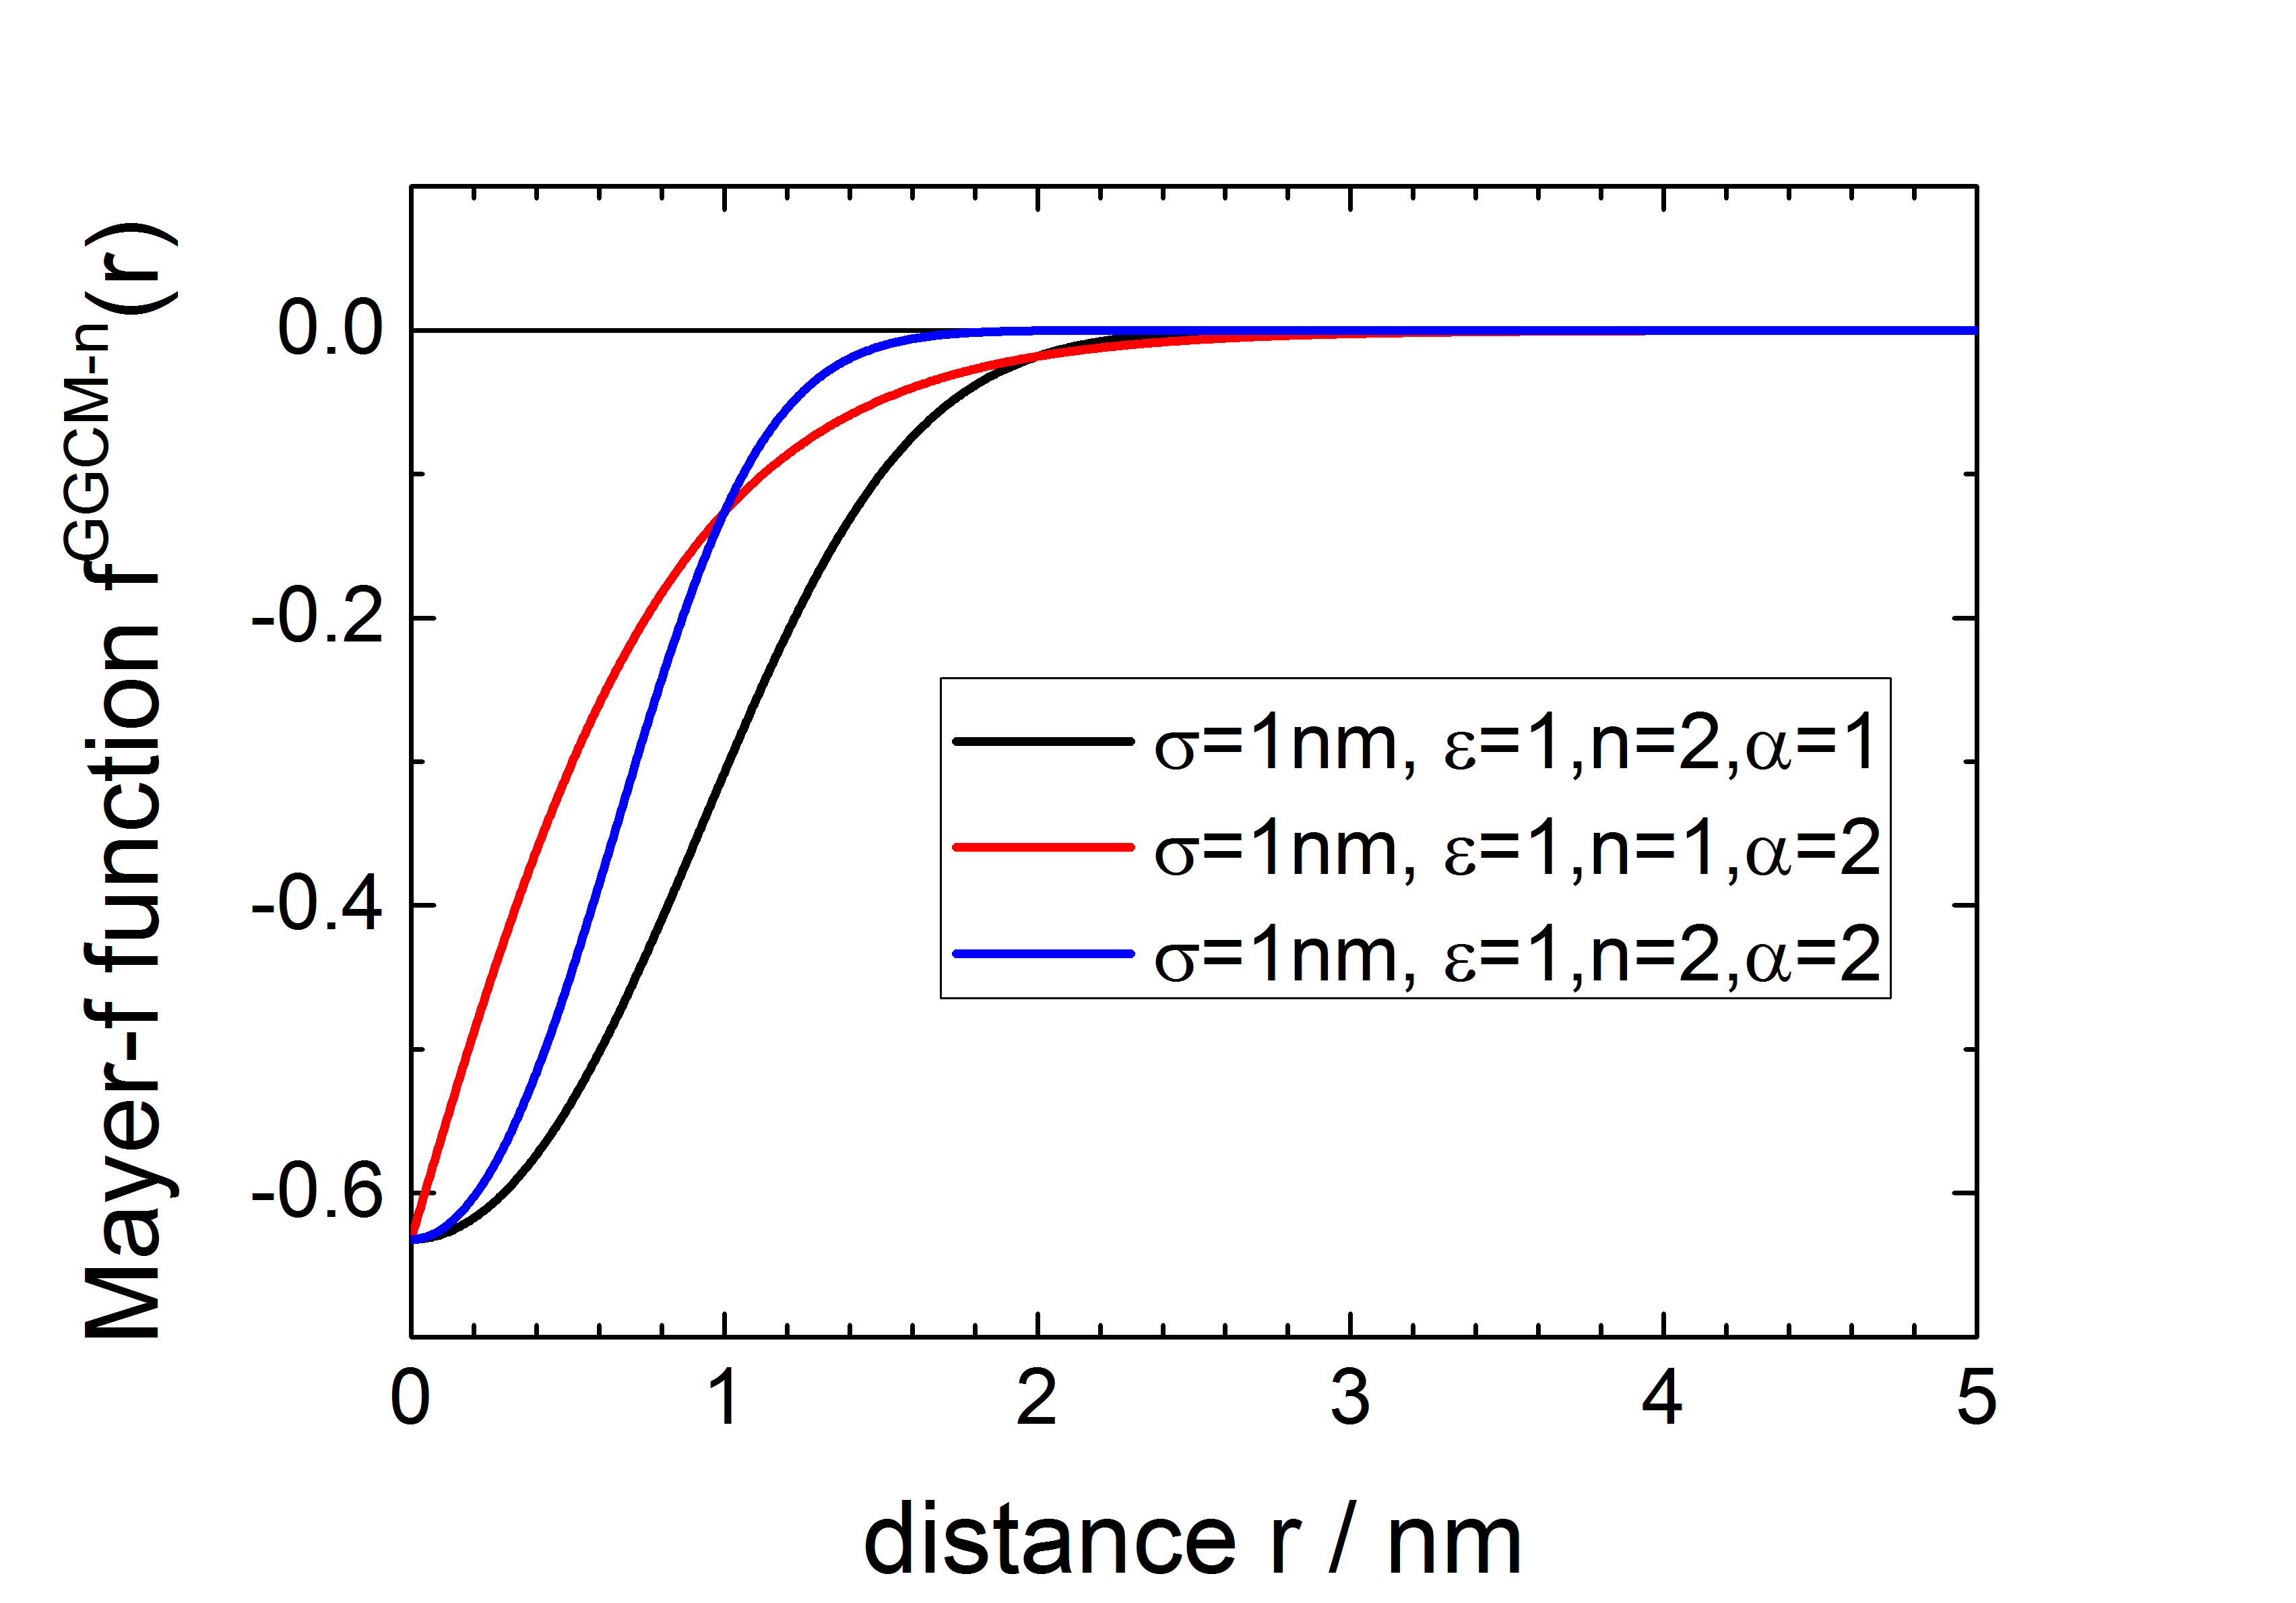
\includegraphics[width=0.45\textwidth,height=0.314\textwidth]{../images/OZsolver/potentials/potfGGCM-n.png}}
  \caption{potential $u^\text{GGCM-n}(r,\sigma,\ldots)$ and it's Mayer-f function $\exp(-u^\text{GGCM-n}(r,\sigma,\ldots)/k_BT)-1$}
\end{figure}


% \vphantom{.}~\\
\newpage
\subsection{Fermi Distribution Model}
~\\
\begin{align}
u^\text{FDM}(r,\sigma,\epsilon,\xi) &=
k_\text{B} T \epsilon
\frac{1+\exp\left(-\sigma/\xi\right)}{1+\exp\left(\left(r-\sigma\right)/\xi\right)}
\end{align}
For $\xi = 0$ the Fermi Potential goes over into the Penetrable Sphere Model.

\begin{figure}[htb]
\centering
  \subfigure[Fermi potential $u^\text{Fermi}(r,\sigma,\ldots)$]{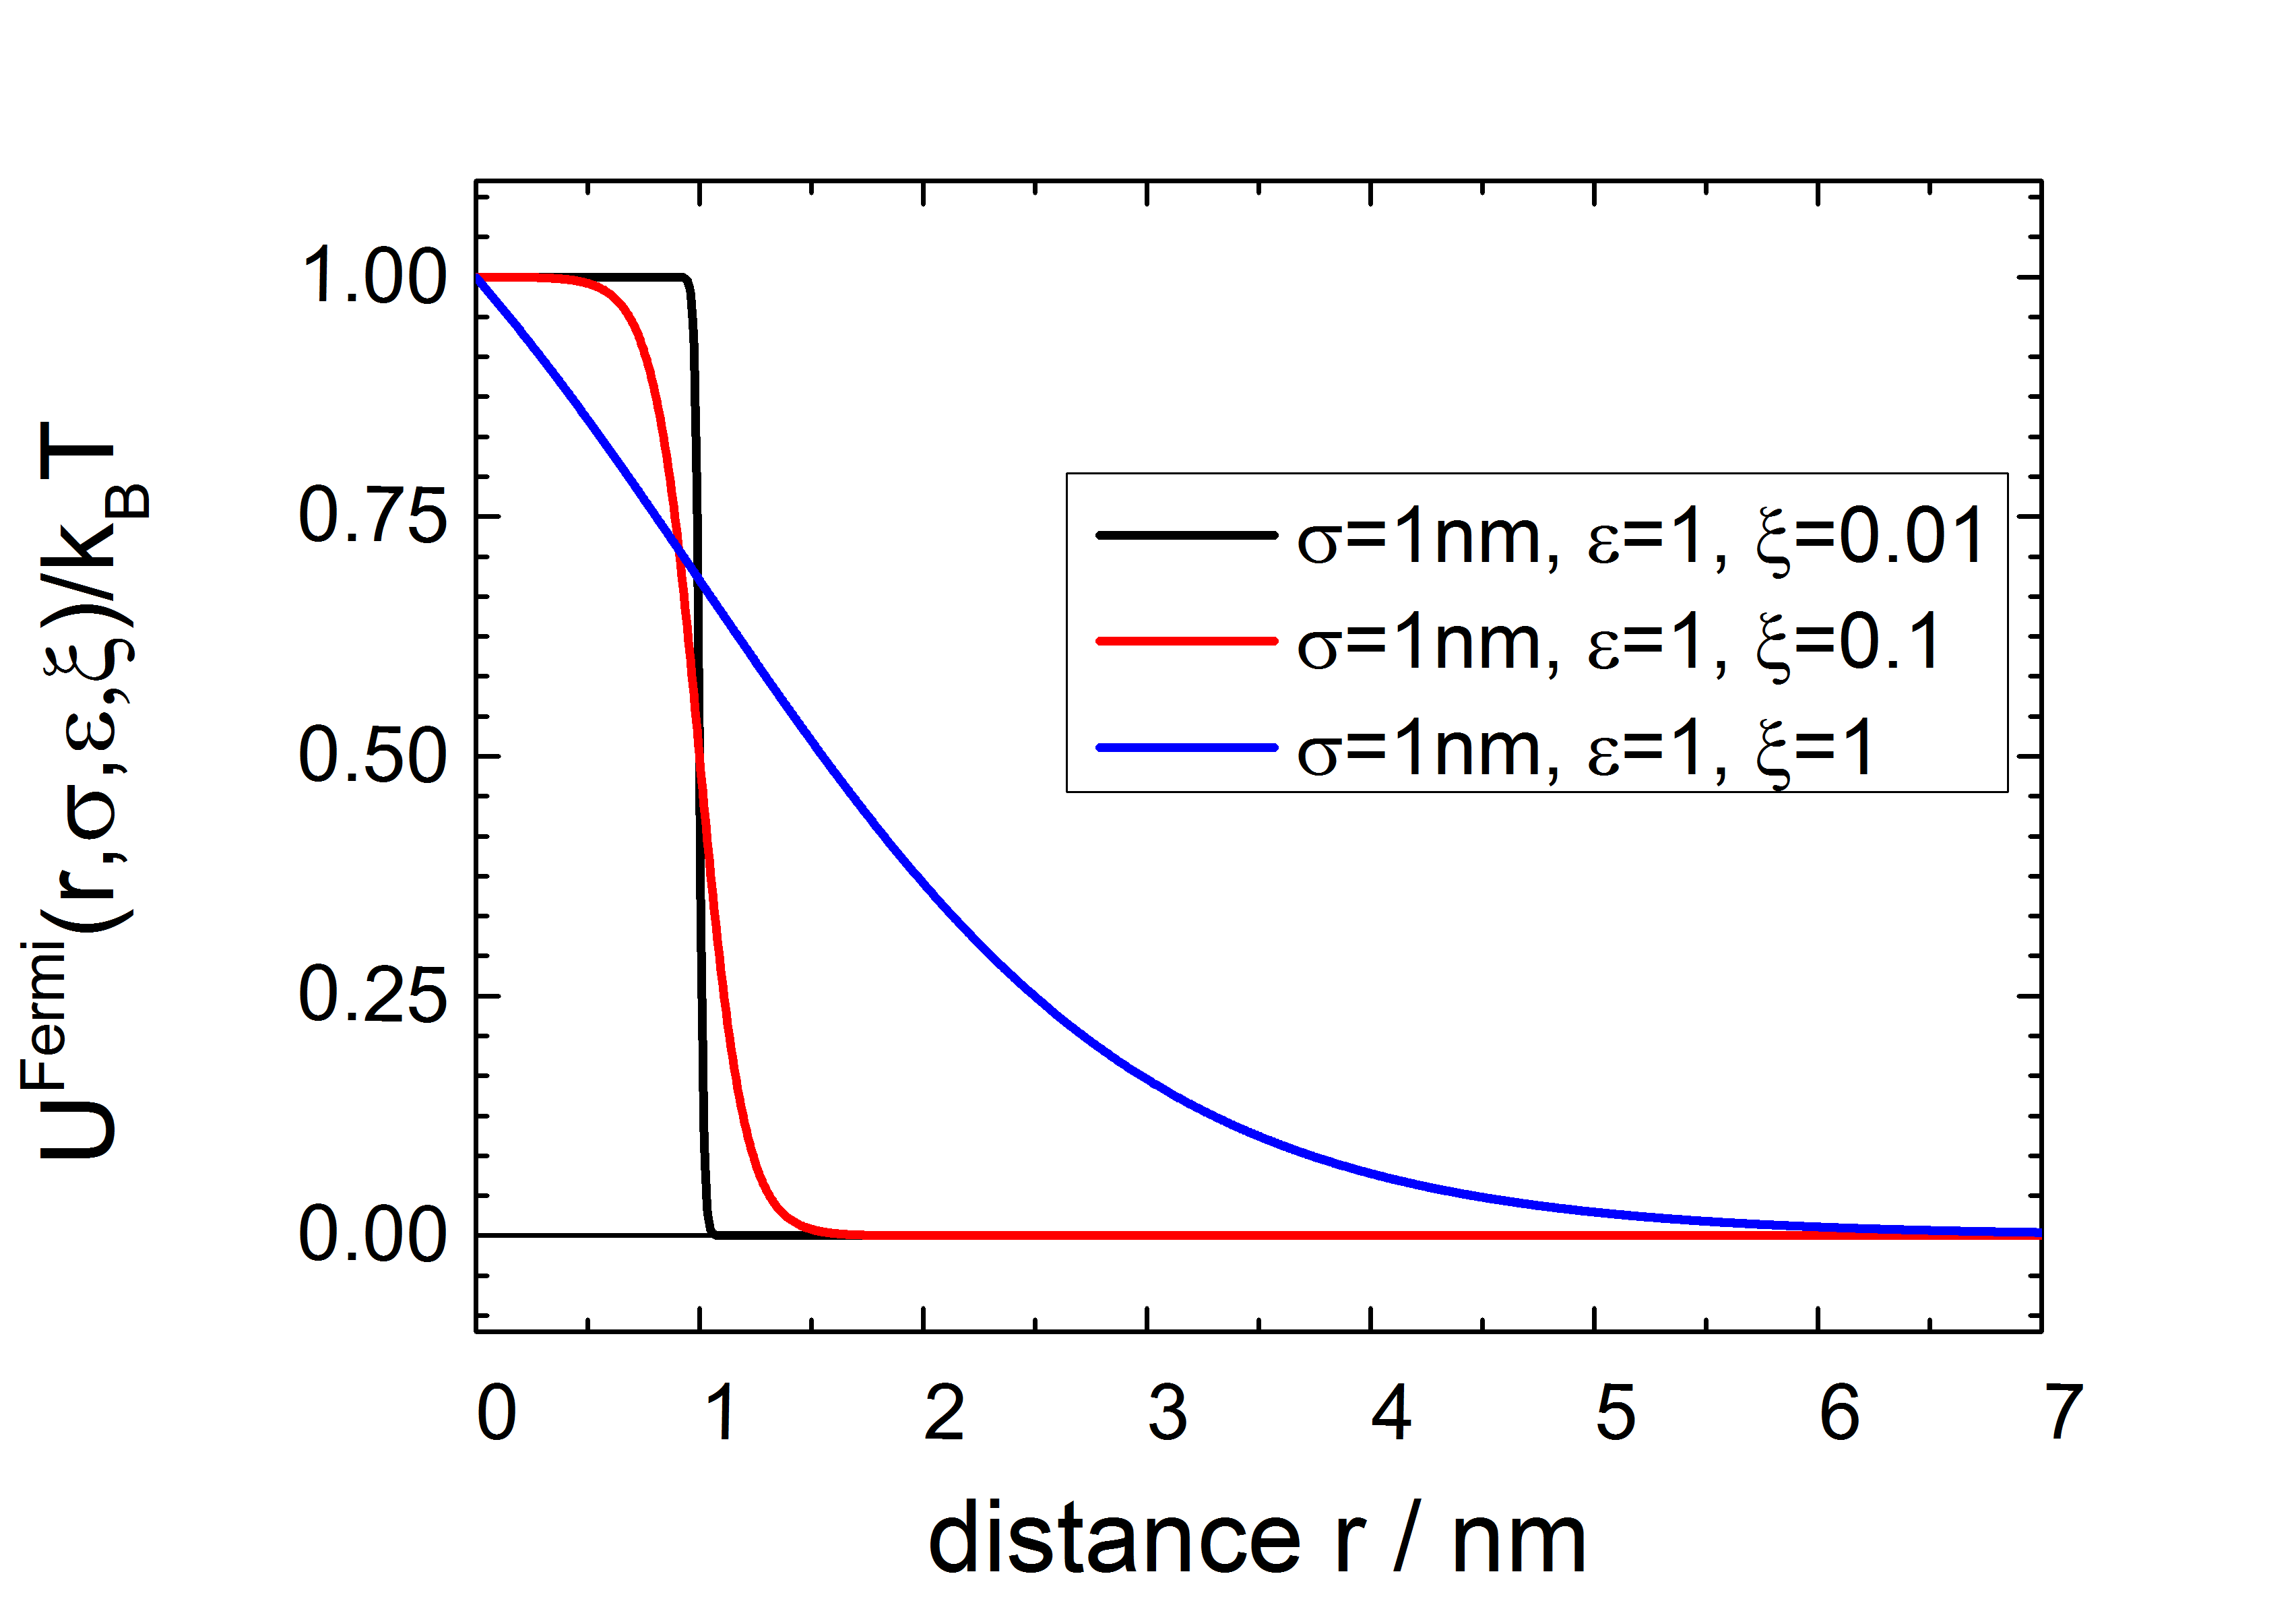
\includegraphics[width=0.45\textwidth,height=0.314\textwidth]{../images/OZsolver/potentials/potUFermi.png}}
  \quad
  \subfigure[Mayer-f function of $u^\text{Fermi}(r,\sigma,\ldots)$]{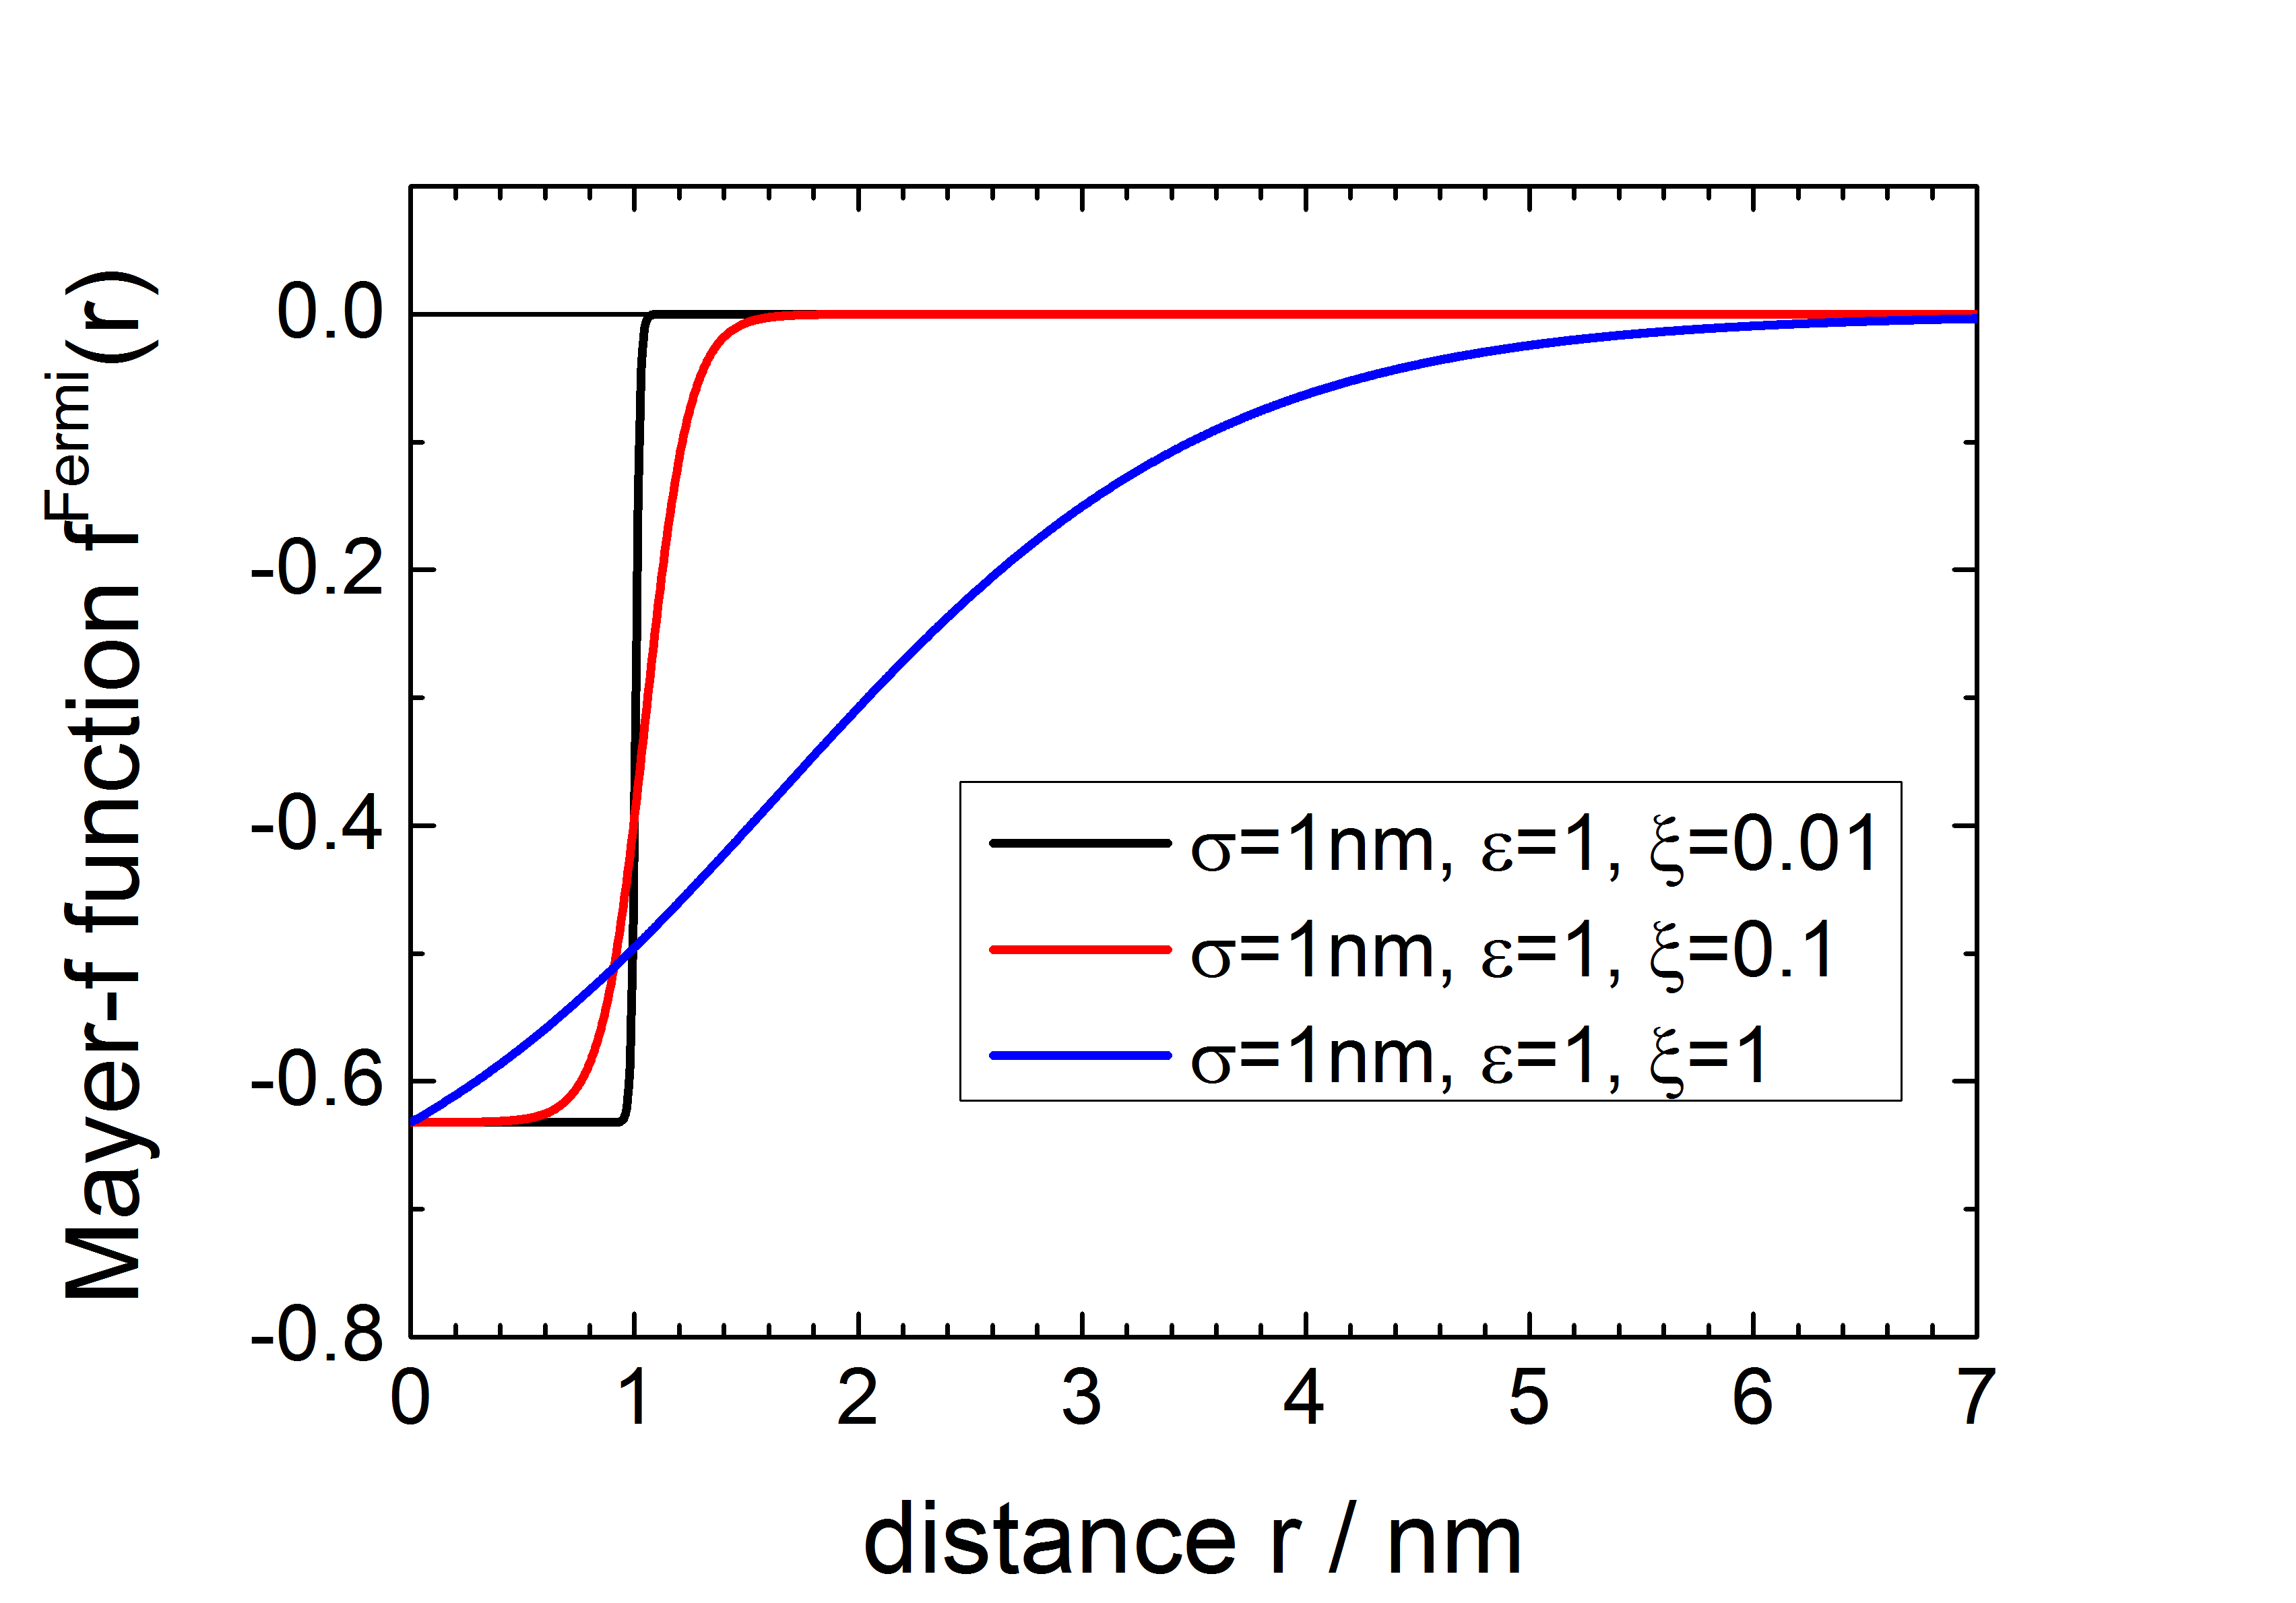
\includegraphics[width=0.45\textwidth,height=0.314\textwidth]{../images/OZsolver/potentials/potfFermi.png}}
  \caption{potential $u^\text{Fermi}(r,\sigma,\ldots)$ and it's Mayer-f function $\exp(-u^\text{Fermi}(r,\sigma,\ldots)/k_BT)-1$}
\end{figure}

\newpage
\subsection{Star Polymer Potential}
~\\

Star polymers with tunable number $f$ and size of arms, and thus interactions,
represent ideal model systems for exploring the regime of soft material behaviour that
interpolates between hard spheres and polymeric coils.
Likos et al.\ \cite{Likos1998,Likos2001} have proposed an effective potential that describes
the interaction between two stars. The potential is given by
\begin{align}\
\label{eq:star1_potential}
u^\text{star1}(r,\sigma,f) &=
k_\text{B} T \frac{5}{8} f^{3/2}
\begin{cases}
\left(\frac{1}{1+\sqrt{f}}-\ln\left(\frac{r}{\sigma}\right) \right)
          & \mbox{for } r \leq \sigma \\
\frac{1}{1+\sqrt{f}} \frac{\sigma}{r}
\exp\left(-\frac{\sqrt{f} (r-\sigma)}{2\sigma}\right)
          & \mbox{for } r >    \sigma
\end{cases}
\end{align}
where $\sigma$ is the effective corona diameter
(e.g., $\sigma \propto f^{1/5} N_a^{3/5}$ for good
solvents, $N_a$ being the arm degree of polymerization and $f$ the functionality of the star).
In equation \ref{eq:star1_potential} above, $\sigma/2$ is a length scale that extends from the
star center to the middle of the outermost Daoud–Cotton
blob \cite{Likos2006}. Extensive comparisons with simulations have
set this scale to $\sigma \cong 1.32R_g$, where $R_g$ is the star radius of
gyration. The effective potential shows a soft, logarithmic
divergence at close approaches, followed by a crossover to a
Yukawa form as the center-to-center separation $r$ grows. The
potential becomes harder with increasing $f$, tending eventually to a hard-sphere
interaction formally obtained in the limit $f\rightarrow\infty$.

\begin{figure}[htb]
\centering
  \subfigure[Star potential $u^\text{star1}(r,\sigma,f)$]{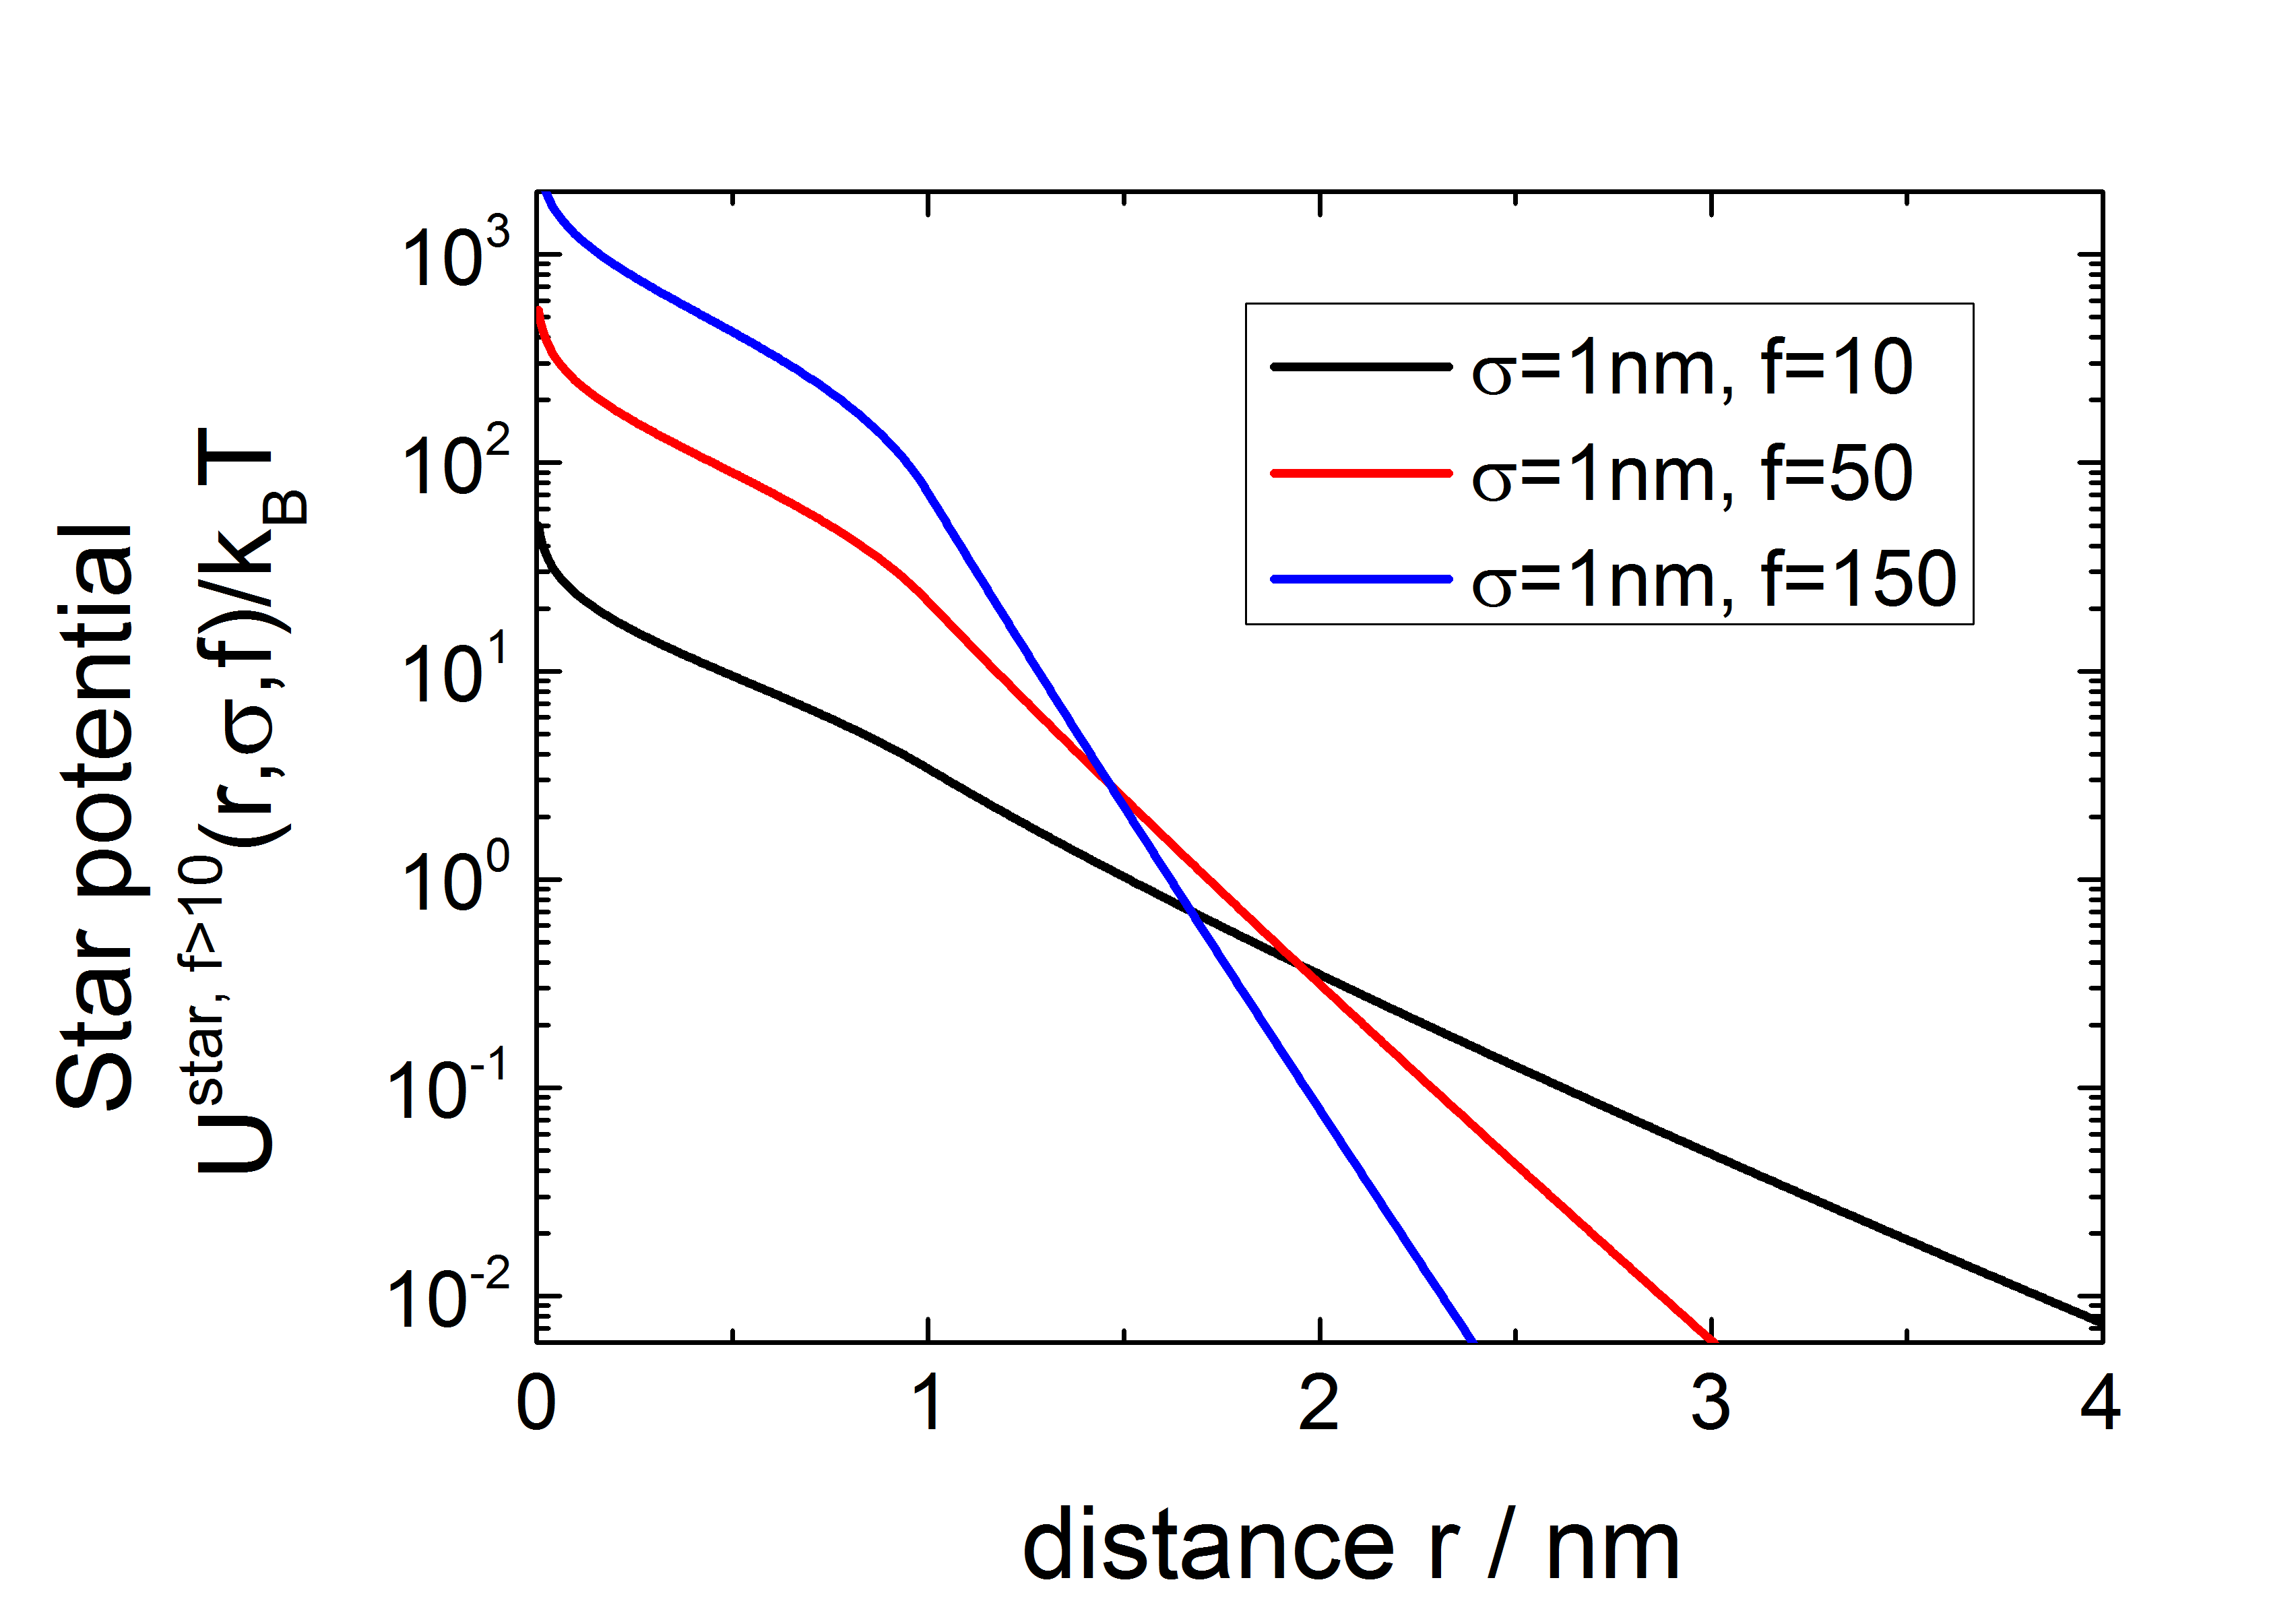
\includegraphics[width=0.45\textwidth,height=0.314\textwidth]{../images/OZsolver/potentials/potUStarfGT10.png}}
  \quad
  \subfigure[Mayer-f function of $u^\text{star1}(r,\sigma,f)$]{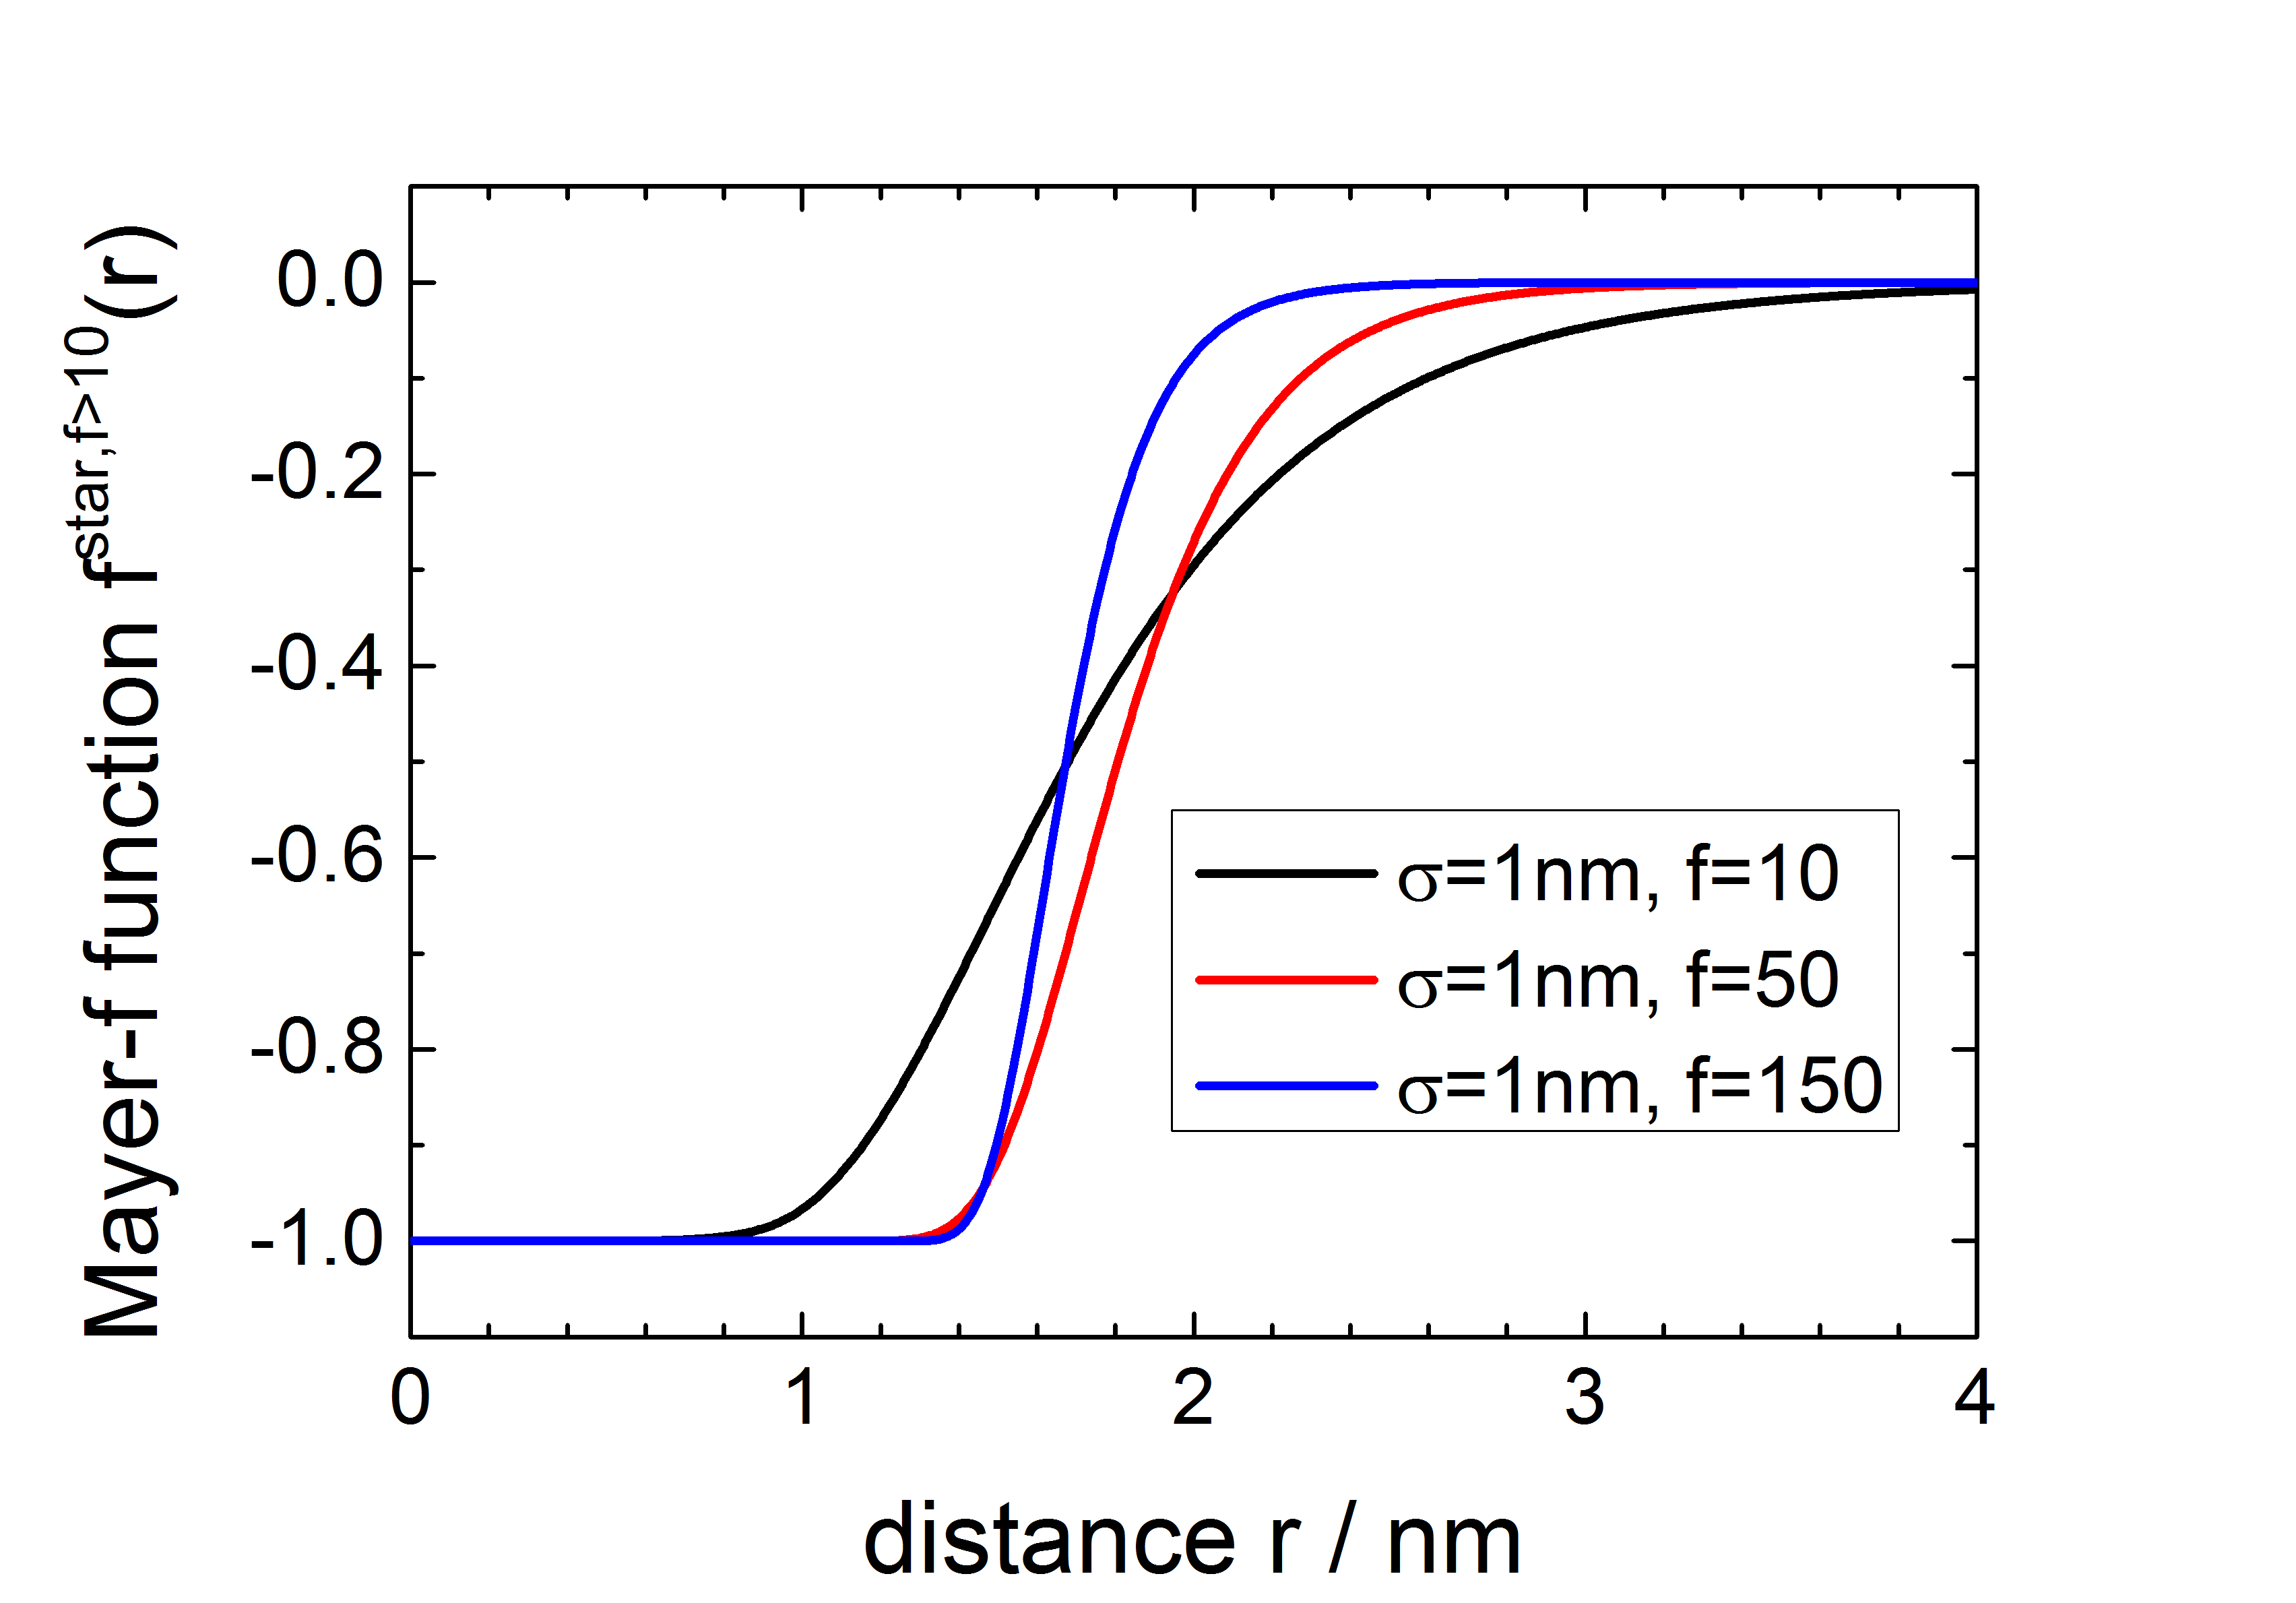
\includegraphics[width=0.45\textwidth,height=0.314\textwidth]{../images/OZsolver/potentials/potfStarfGT10.png}}
  \caption{potential $u^\text{star1}(r,\sigma)$ and it's Mayer-f function $\exp(-u^\text{star1}(r,\sigma,f)/k_BT)-1$}
\end{figure}

The effective potential valid for $f\leq 10$ has the form
\cite{Jusufi2001,Dzubiella2001,Likos2001}:
\begin{align}
u^\text{star2}(r,\sigma,f) &=
k_\text{B} T \frac{5}{8} f^{3/2}
\begin{cases}
\left(\frac{1}{2\tau^2\sigma^2}-\ln\left(\frac{r}{\sigma}\right) \right)
          & \mbox{for } r \leq \sigma \\
\frac{1}{2\tau^2\sigma^2}
\exp\left(-\tau^2(r^2-\sigma^2)\right)
          & \mbox{for } r >    \sigma
\end{cases} \\
\mbox{with } \tau &= \left(\frac{1.12}{3\sigma}-\frac{1.03}{3\sigma}\right)f+\frac{1.03}{\sigma}
\end{align}
$\tau$ is a free parameter of the order and is obtained by fitting to computer
simulation results \cite{Dzubiella2001}.

\begin{figure}[htb]
\centering
  \subfigure[Star potential for $u^\text{star2}(r,\sigma,f)$]{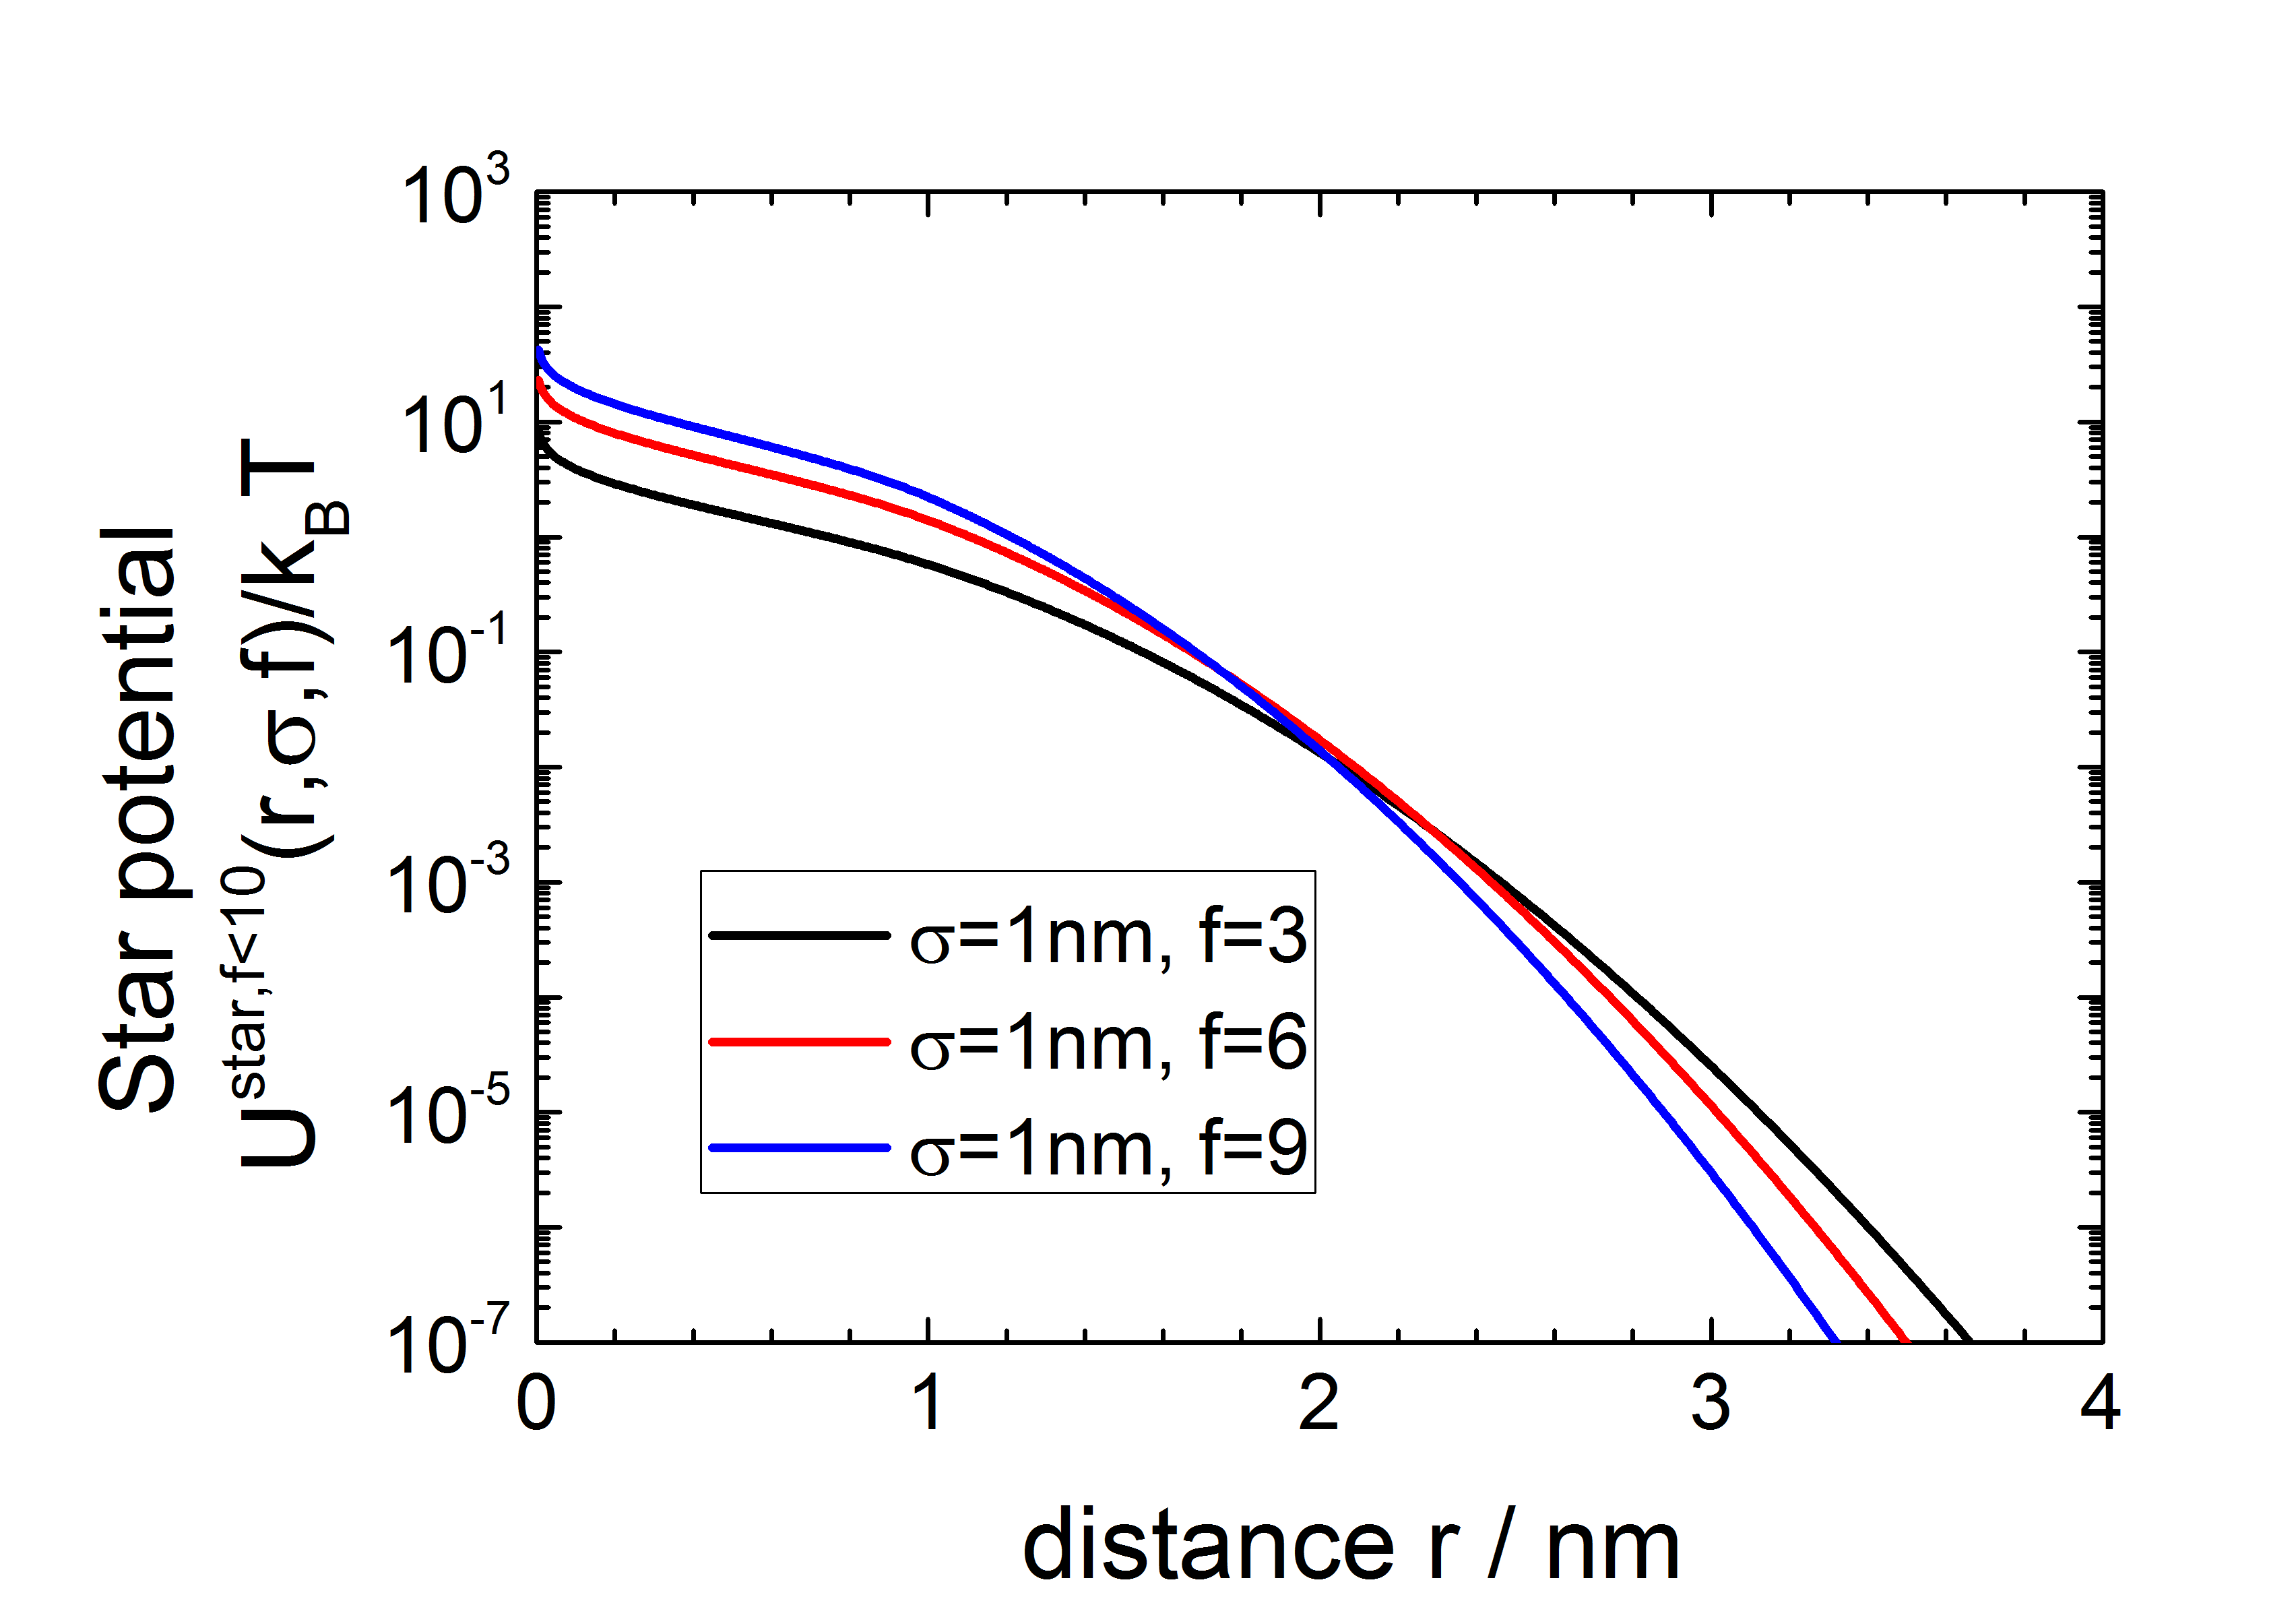
\includegraphics[width=0.45\textwidth,height=0.314\textwidth]{../images/OZsolver/potentials/potUStarfLT10.png}}
  \quad
  \subfigure[Mayer-f function of $u^\text{star2}(r,\sigma,f)$]{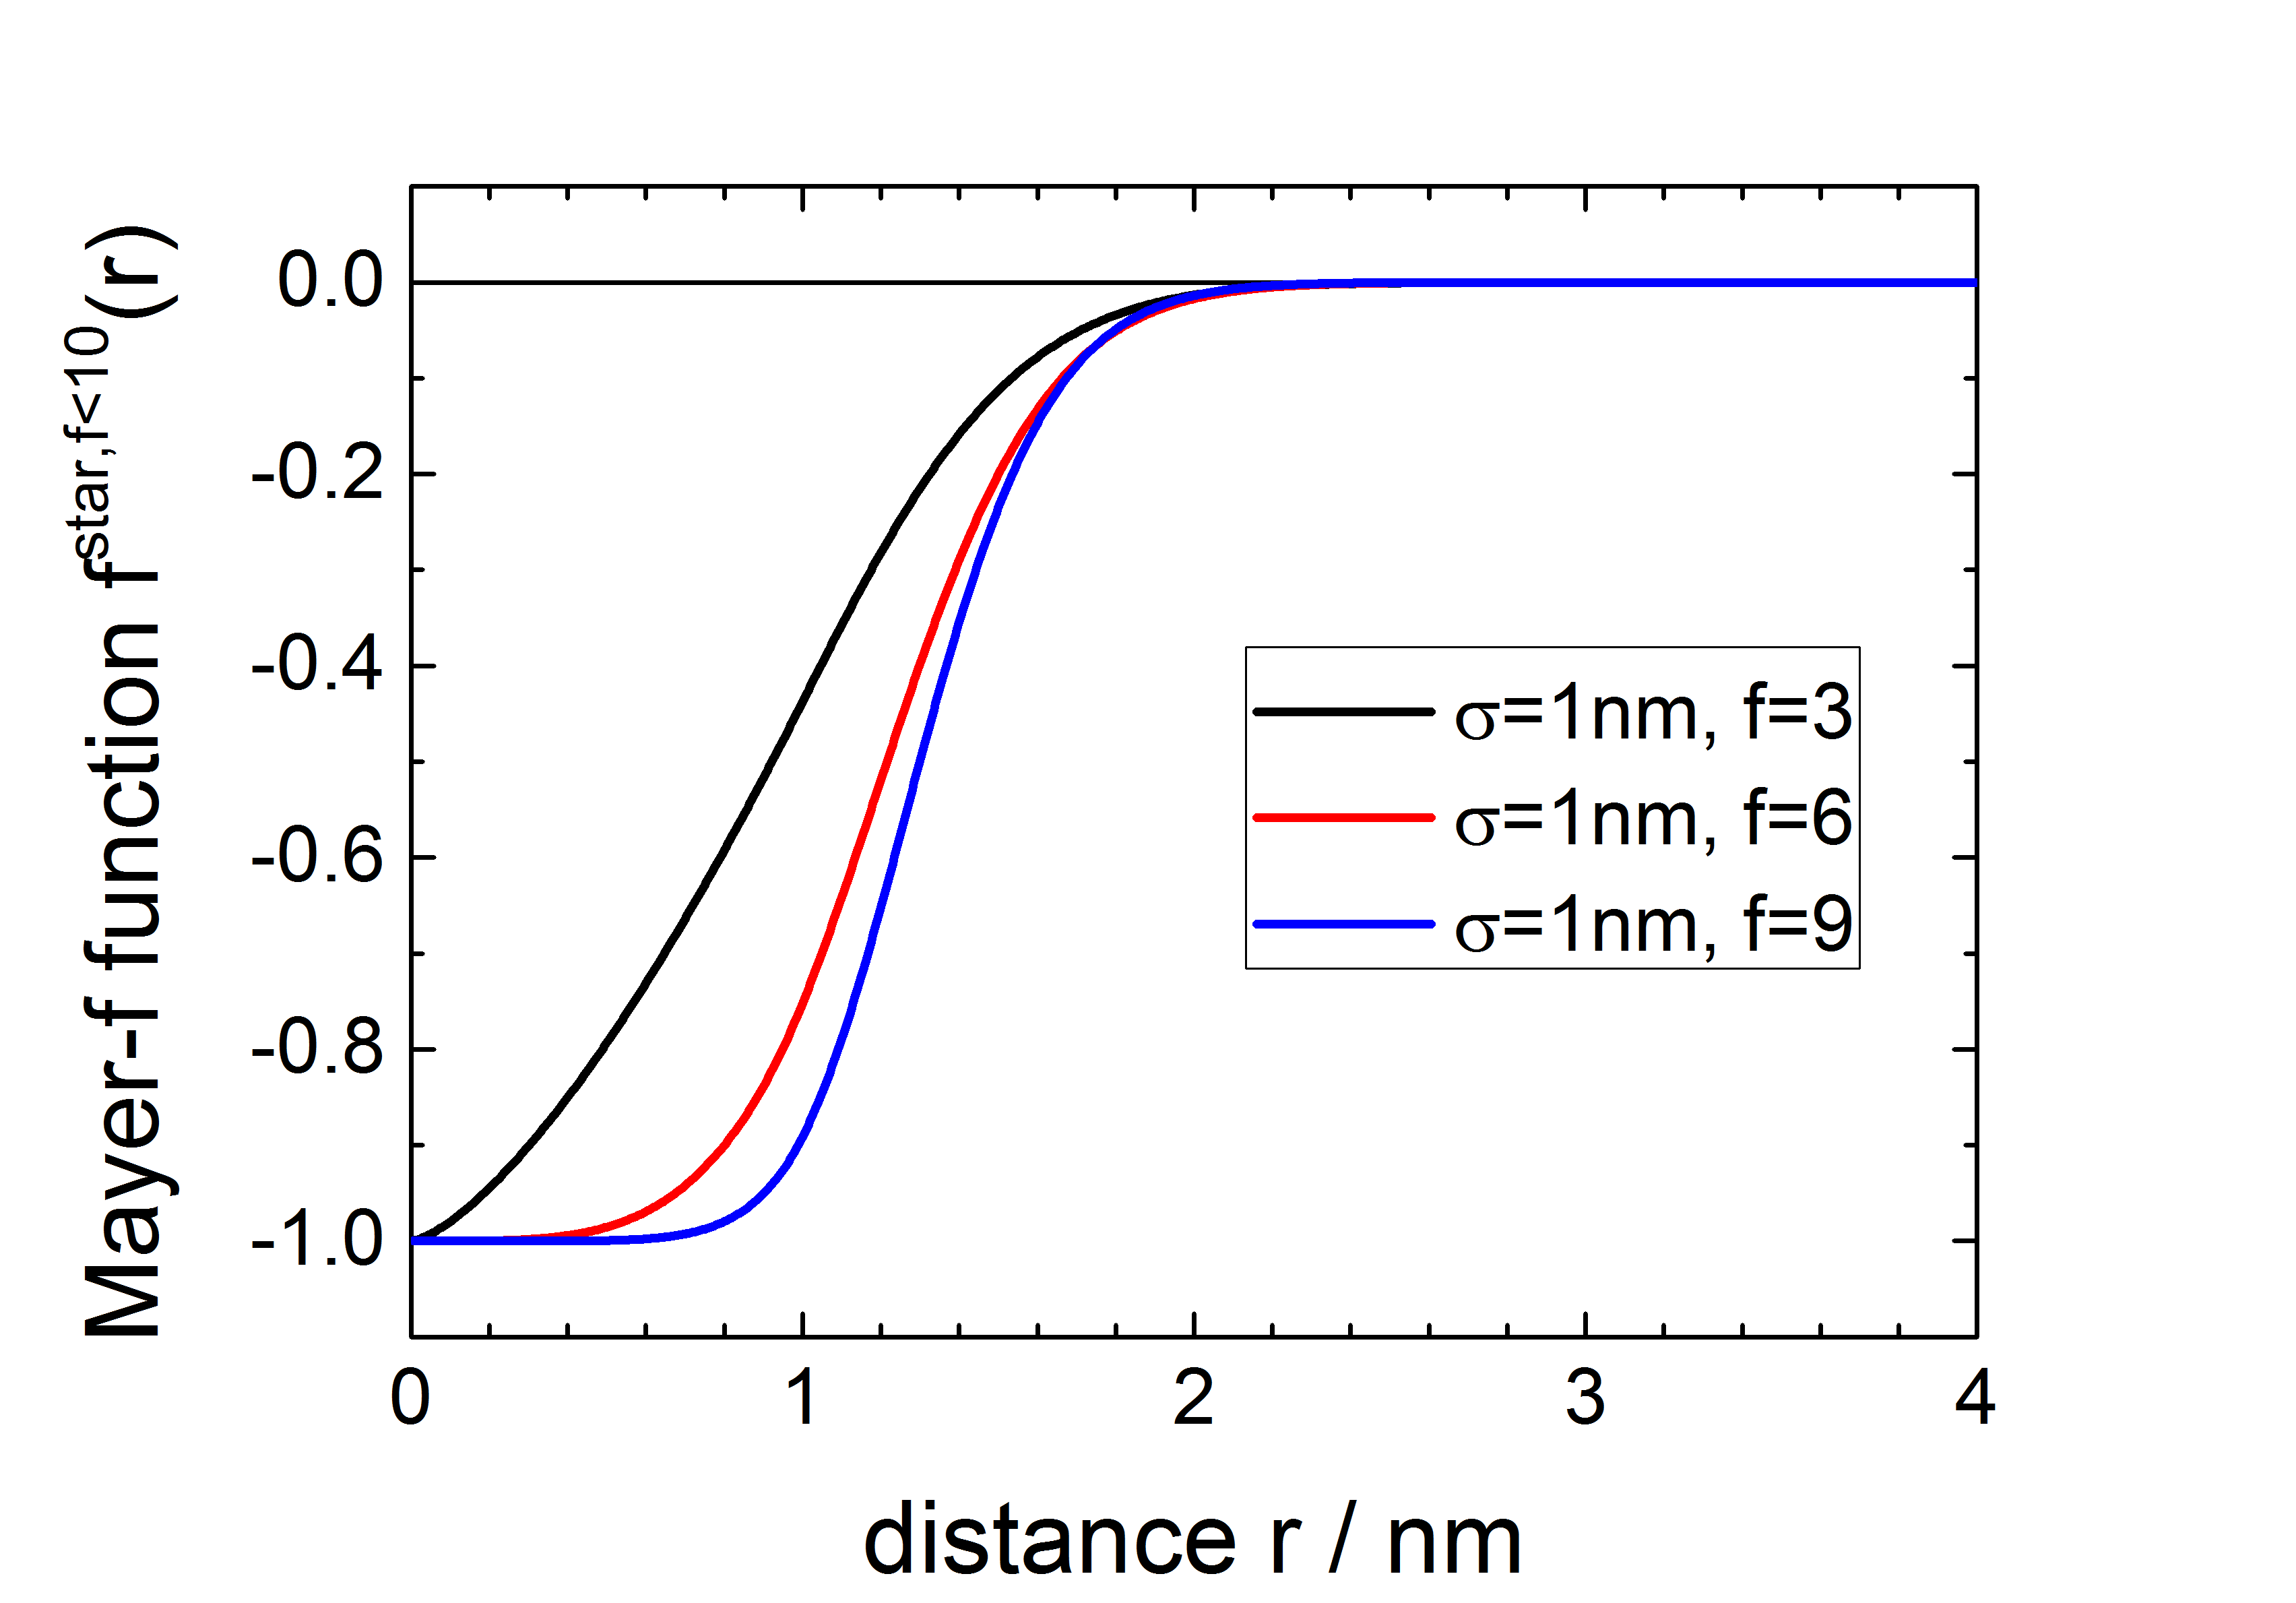
\includegraphics[width=0.45\textwidth,height=0.314\textwidth]{../images/OZsolver/potentials/potfStarfLT10.png}}
  \caption{potential $u^\text{star2}(r,\sigma)$ and it's Mayer-f function $\exp(-u^\text{star2}(r,\sigma,f)/k_BT)-1$}
\end{figure}

% \vphantom{.}~\\
\newpage
\subsection{Lennard-Jones Potential}
~\\

The Lennard-Jones potential is a mathematically simple model that approximates the interaction
between a pair of neutral atoms or molecules.
A form of the potential was first proposed in 1924 by John Lennard-Jones \cite{Jones1924}.
\begin{align}
u^\text{LJ}(r,\sigma,\ldots) &= 4 k_\text{B}T \epsilon \left[ \left(\frac{\sigma}{r}\right)^{12} - \left(\frac{\sigma}{r}\right)^{6}\right]
\end{align}
The Lennard-Jones (LJ) potential has a minimum at $r_m=2^{1/6} \sigma$, so that the potential can be written in parts of
\begin{align}
u^\text{LJ}_\text{ref}(r) & \equiv 0 \\
u^\text{LJ}_\text{SR}(r)  & = u^\text{LJ}_\text{R}(r) =
\begin{cases}
u^\text{LJ}(r) - u^\text{LJ}(r_m)  & \mbox{if } r <    rm \\
0                                  & \mbox{if } r \geq rm
\end{cases}
\end{align}
and
\begin{align}
u^\text{LJ}_\text{pert}(r) &= u^\text{LJ}(r) \\
u^\text{LJ}_\text{LR}(r)   &= u^\text{LJ}_\text{A}(r) =
\begin{cases}
u^\text{LJ}(r_m)          & \mbox{if } r <    rm \\
u^\text{LJ}_\text{LR}(r)  & \mbox{if } r \geq rm
\end{cases}
\end{align}
The LJ potential is not splitted in a reference and perturbation part, i.e. the reference part is set to 0.

\begin{figure}[htb]
\centering
  \subfigure[Lennard-Jones potential $u^\text{LJ}(r,\sigma,\ldots)$]{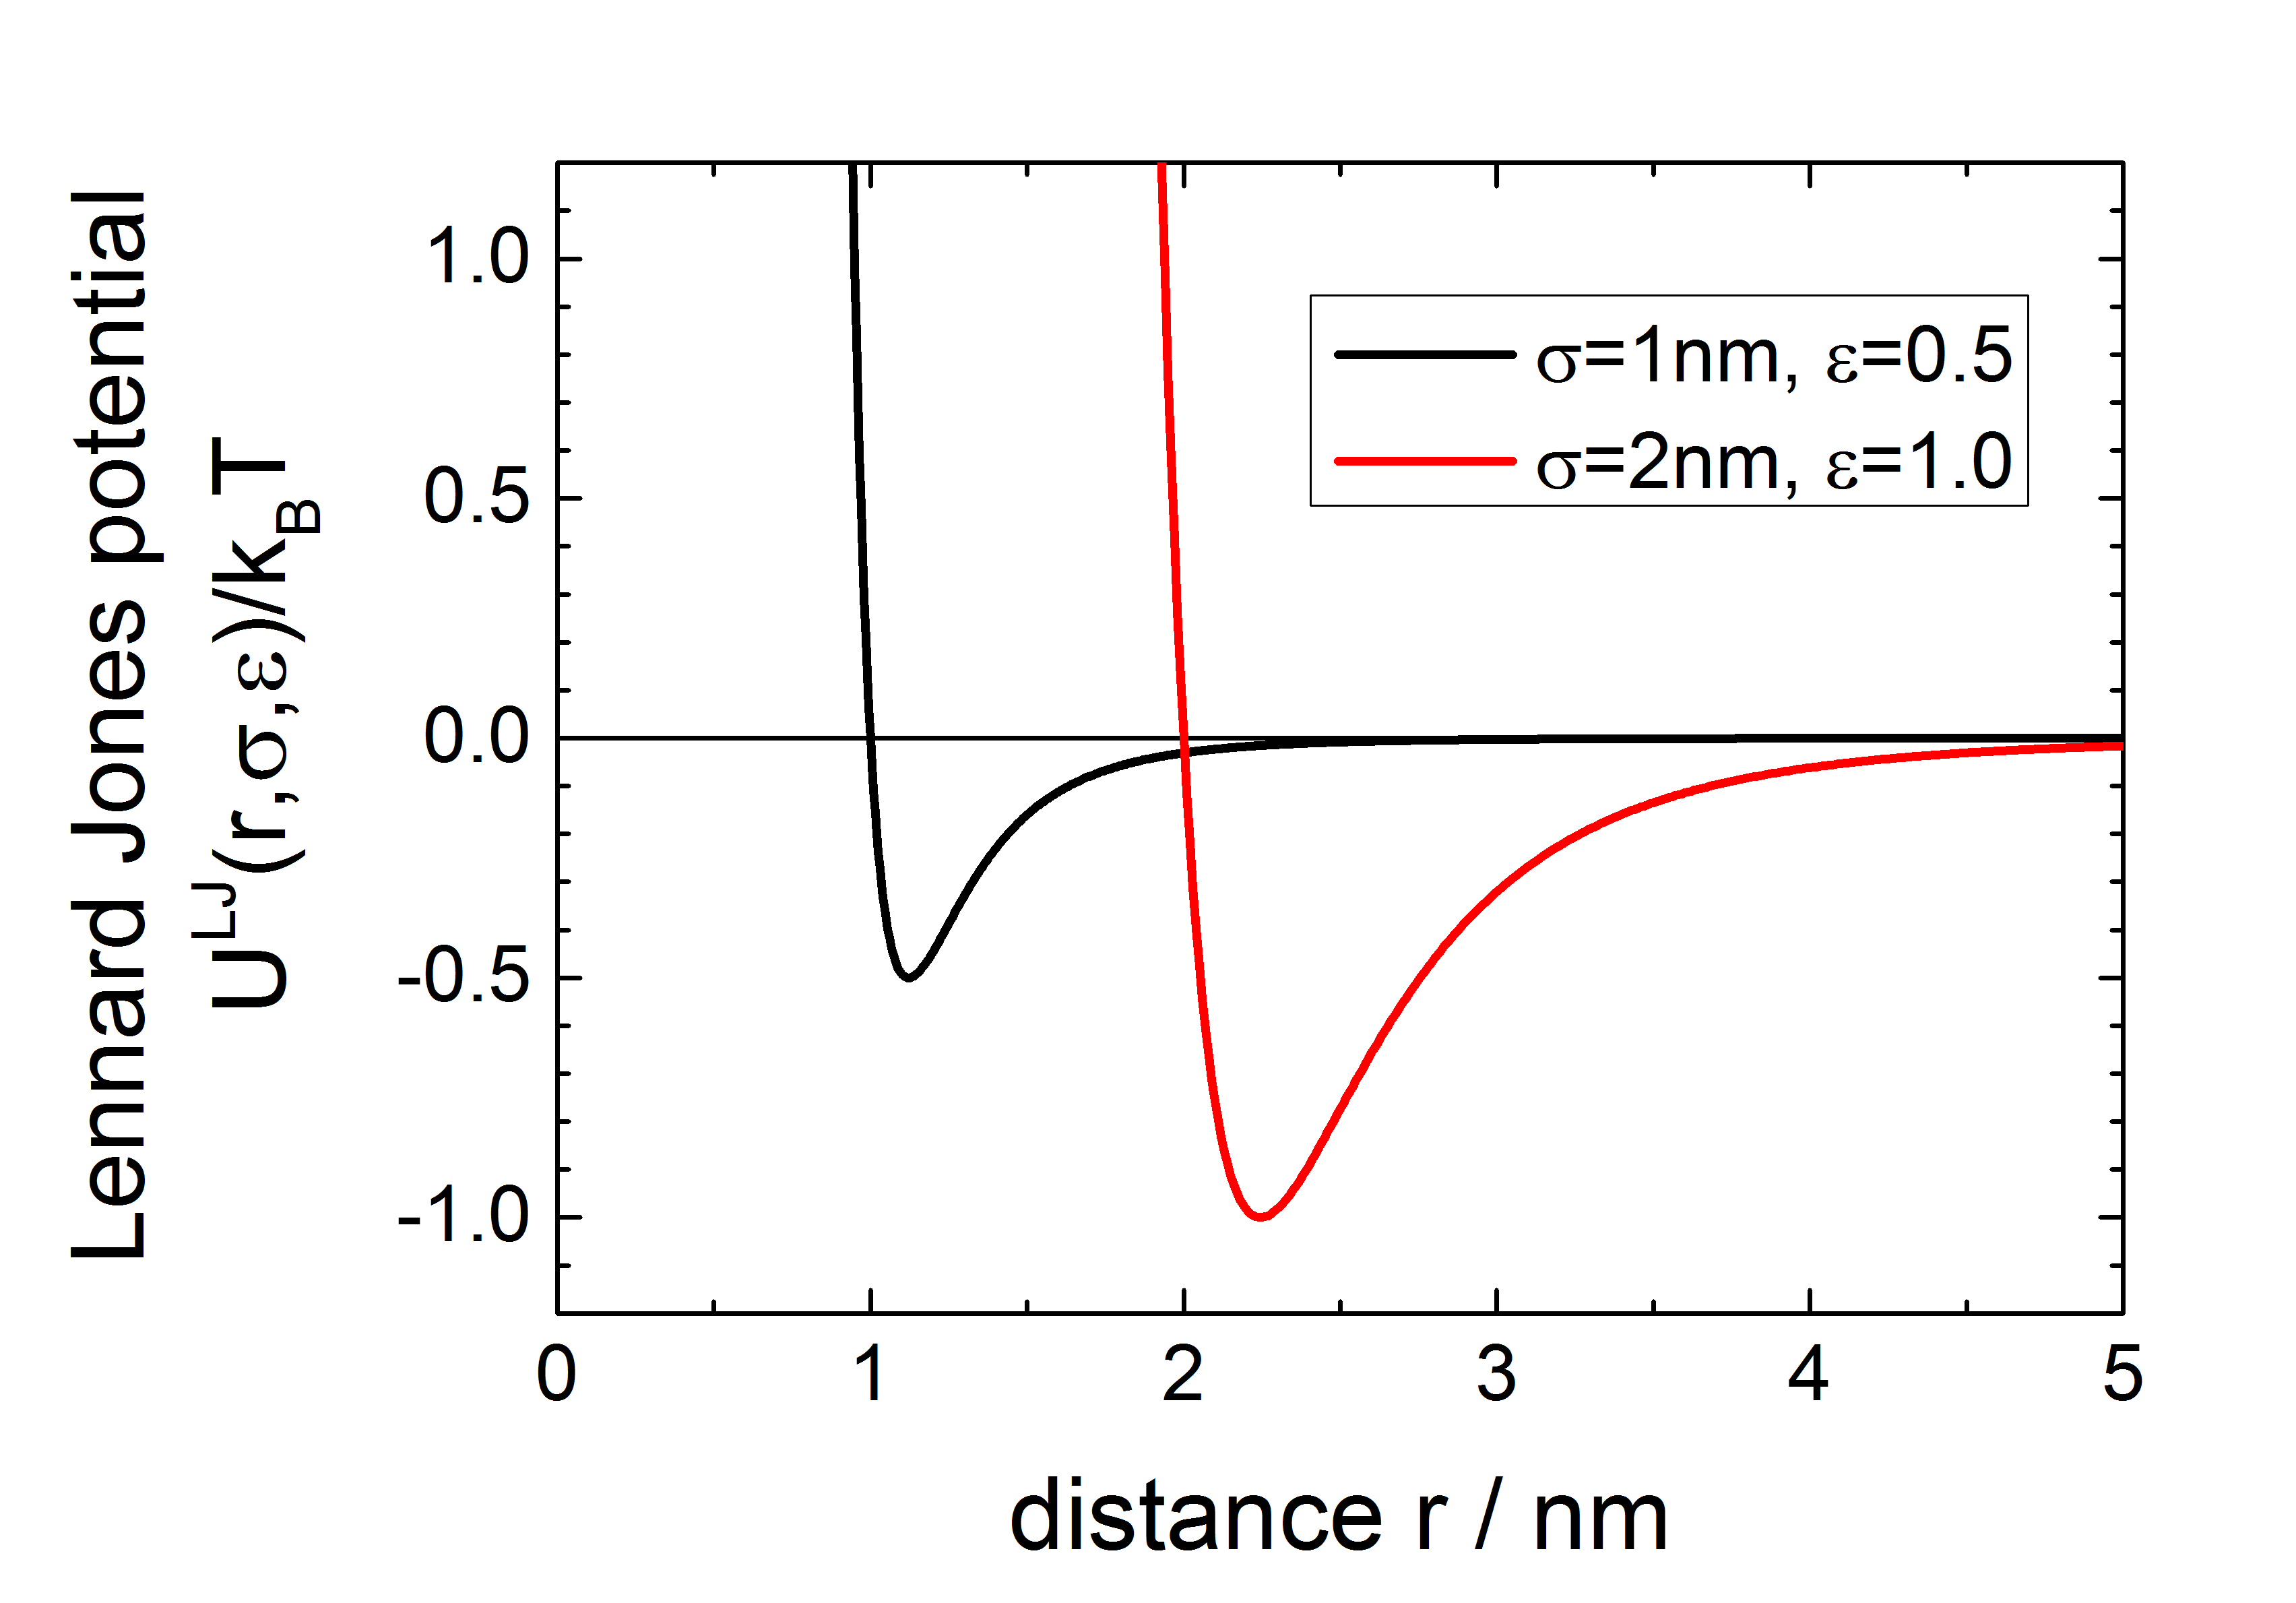
\includegraphics[width=0.45\textwidth,height=0.314\textwidth]{../images/OZsolver/potentials/potULennardJones.png}}
  \quad
  \subfigure[Mayer-f function of $u^\text{LJ}(r,\sigma,\ldots)$]{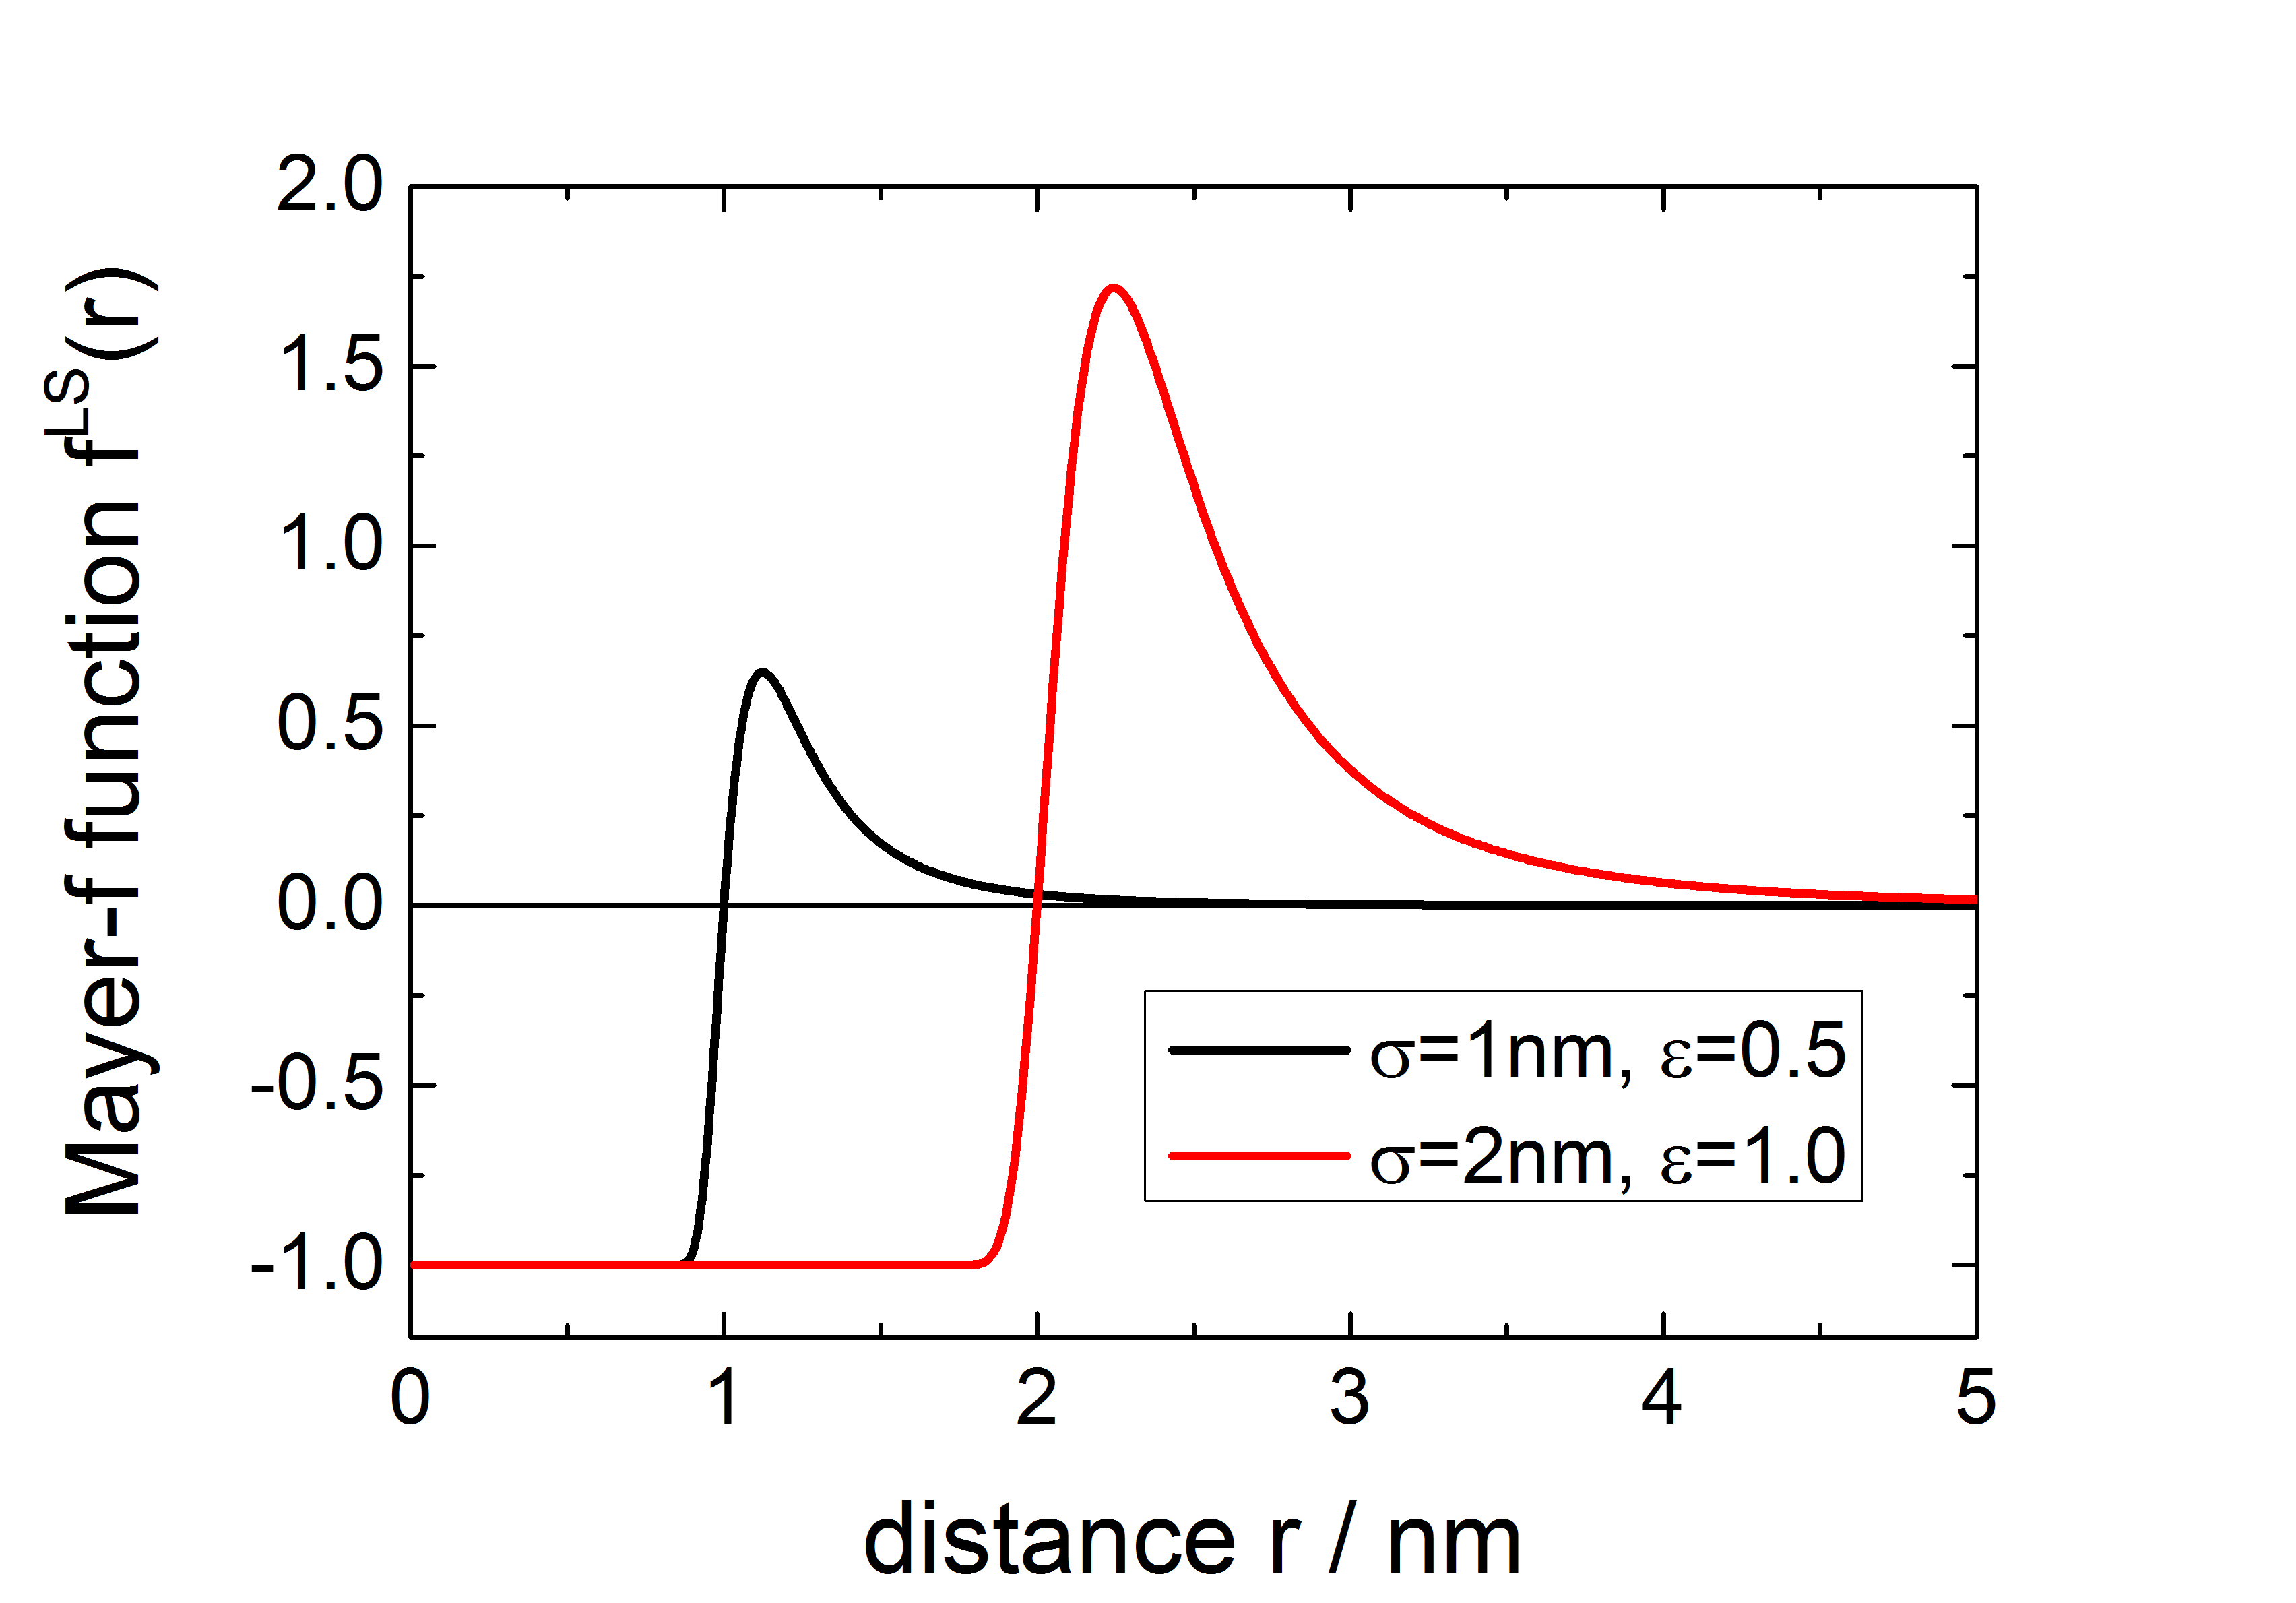
\includegraphics[width=0.45\textwidth,height=0.314\textwidth]{../images/OZsolver/potentials/potfLennardJones.png}}
  \caption{potential $u^\text{LJ}(r,\sigma,\ldots)$ and it's Mayer-f function $\exp(-u^\text{LJ}(r,\sigma,\ldots)/k_BT)-1$}
\end{figure}

% \vphantom{.}~\\
\newpage
\subsection{Depletion Potential}
~\\

The pair interaction potential of spheres by a depleting agent is implemented depending on the shape of the depleting
agent. Analytical expressions have been developed for
spherical, disc-like or rod-like shapes \cite{Oversteegen2004,Lekkerkerker2011}.
The potential between two large spheres and spherical depleting agents of diameter $l$
is given by
\begin{align}
u^\text{depl}_\text{sph}(r) &= -k_\text{B} T (N_\text{I}+N_\text{II}-N_\text{III}) \\
N_\text{I} &= n_d \frac{2}{3}\left(\frac{l}{2}-\frac{r-\sigma}{2}\right)^2
                \left(\frac{3\sigma}{2}+l+\frac{r-\sigma}{2}\right)\\
N_\text{II} &= N_\text{III} = 0
\end{align}

\begin{figure}[htb]
\centering
  \subfigure[potential between two large spheres and spherical depleting agents $u^\text{depl}_\text{sph}(r,\sigma,\ldots)$]{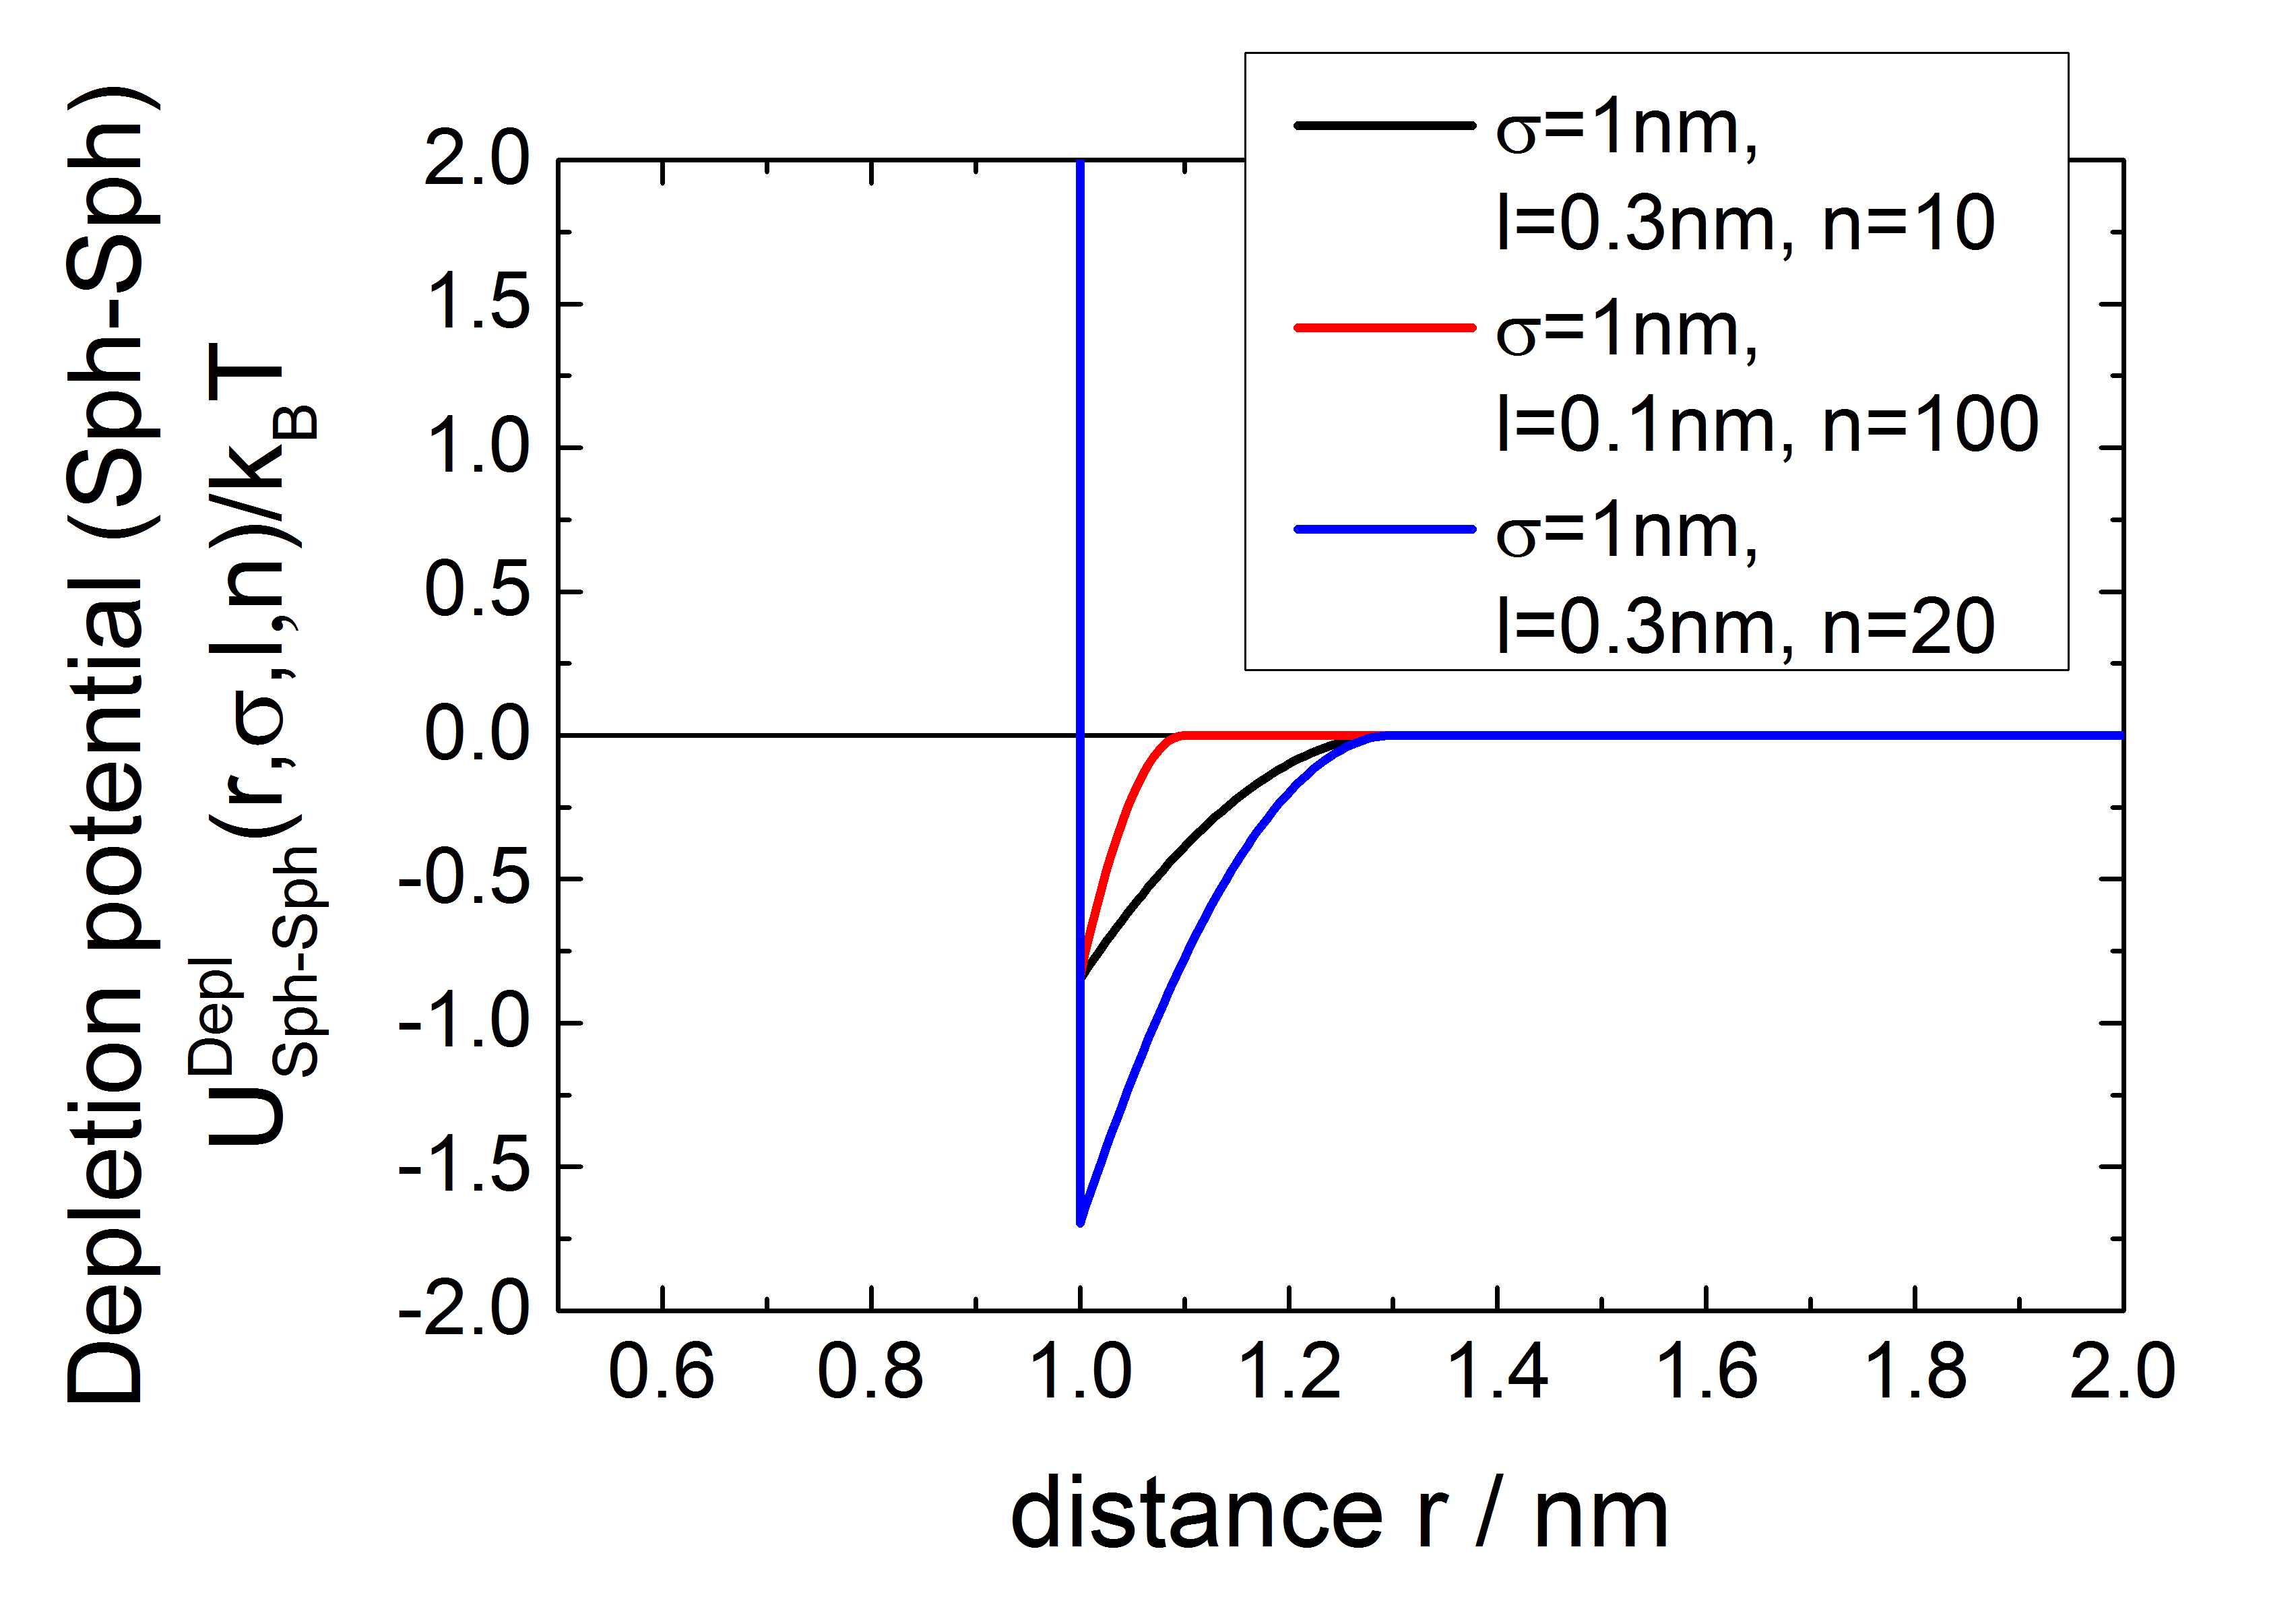
\includegraphics[width=0.45\textwidth,height=0.314\textwidth]{../images/OZsolver/potentials/potUDepl-Sph-Sph.png}}
  \quad
  \subfigure[Mayer-f function of $u^\text{depl}_\text{sph}(r,\sigma,\ldots)$]{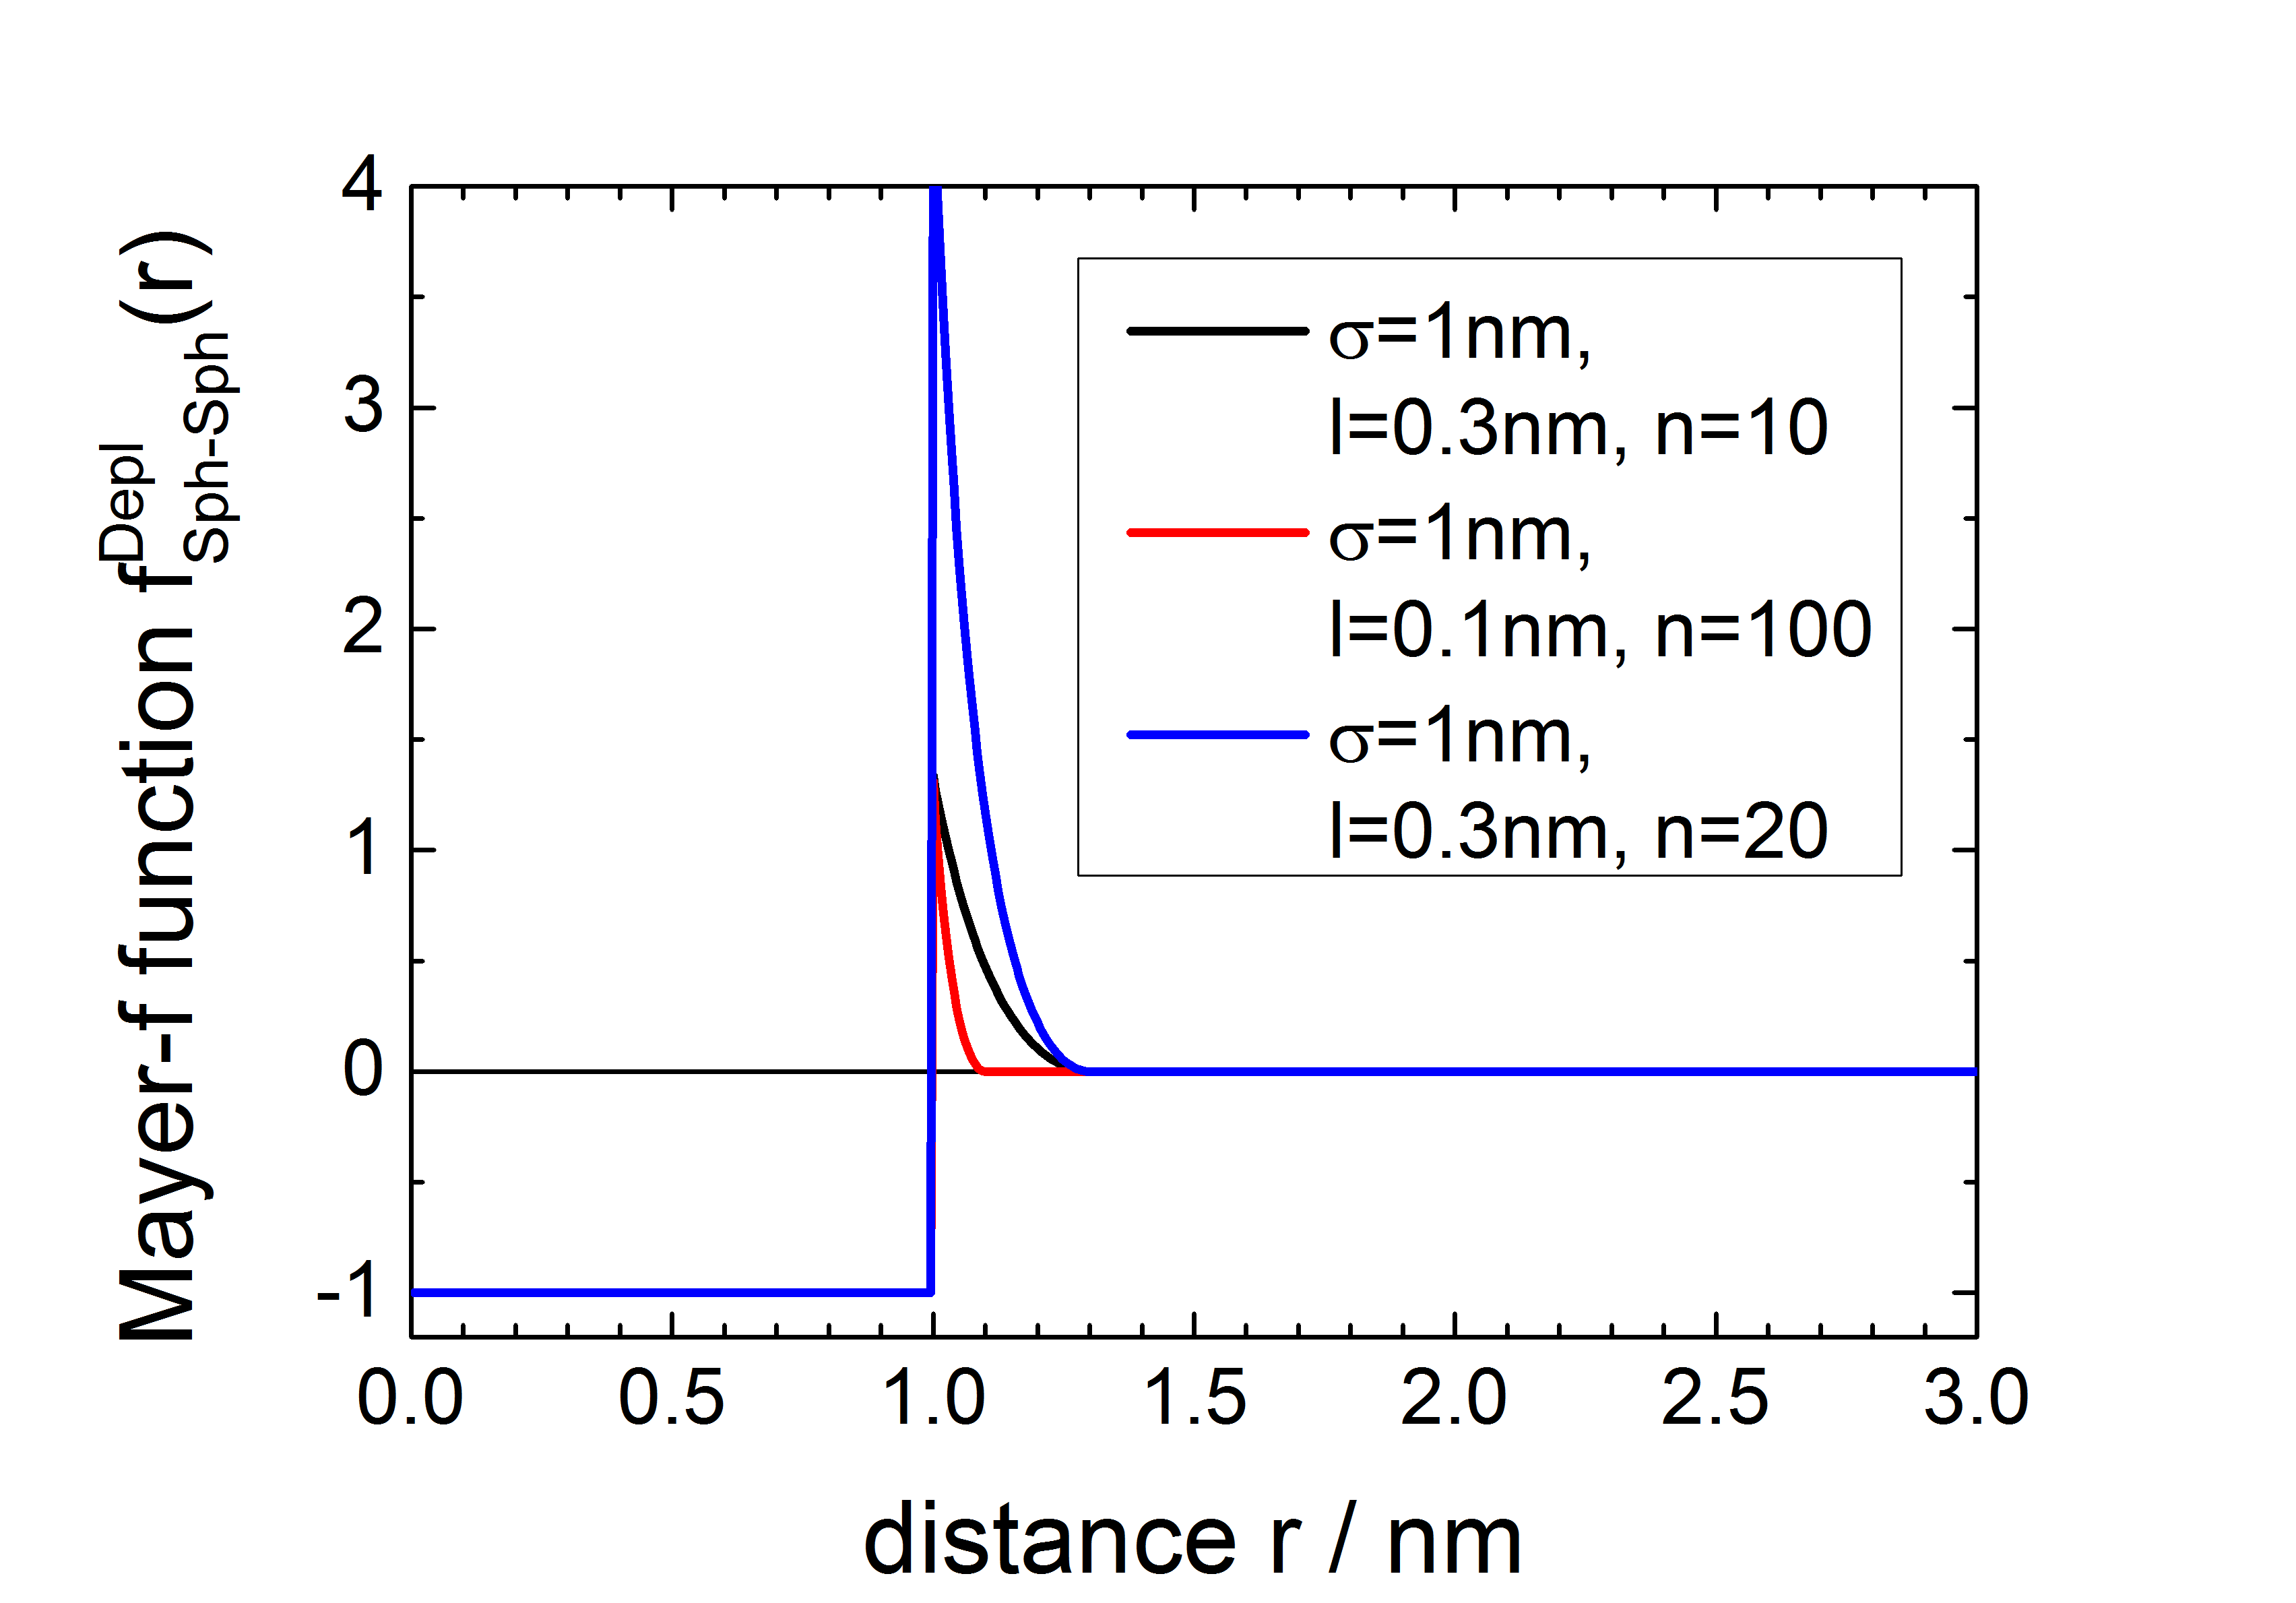
\includegraphics[width=0.45\textwidth,height=0.314\textwidth]{../images/OZsolver/potentials/potfDepl-Sph-Sph.png}}
  \caption{potential $u^\text{depl}_\text{sph}(r,\sigma,\ldots)$ and it's Mayer-f function $\exp(-u^\text{depl}_\text{sph}(r,\sigma,\ldots)/k_BT)-1$}
\end{figure}

The potential between two large spheres and infinitesimal thin discs of diameter $D$
as a depleting agents is given by
\begin{align}
u^\text{depl}_\text{discs}(r) &= -k_\text{B} T (N_\text{I}+N_\text{II}-N_\text{III}) \\
N_\text{I} &= n_d \frac{\pi}{6}\sigma D^2 \left(1-\frac{r-\sigma}{D}\right)^2
                \left(\frac{3}{2}+\frac{D}{\sigma}+\frac{1}{2}\frac{r-\sigma}{\sigma}\right)\\
\begin{split}
N_\text{II} - N_\text{III} &= \frac{\pi}{6} n_d D^2\sigma
                              \left\{ -\frac{3}{2}\left(1-\frac{r-\sigma}{D}\right)^2
                                      -\frac{3}{4}\pi\frac{r-\sigma}{D} \right. \\
                           & \qquad \qquad + \frac{3}{2}\frac{r-\sigma}{D} \arcsin \frac{r-\sigma}{D}  \\
                           & \qquad \qquad + \left.
                              \left(1+\frac{1}{2}\left(\frac{r-\sigma}{D}\right)^2\right)
                                   \sqrt{1-\left(\frac{r-\sigma}{D}\right)^2}
                              \right\}
\end{split}
\end{align}

\begin{figure}[htb]
\centering
  \subfigure[potential between two large spheres and disclike depleting agents $u^\text{depl}_\text{discs}(r,\sigma,\ldots)$]{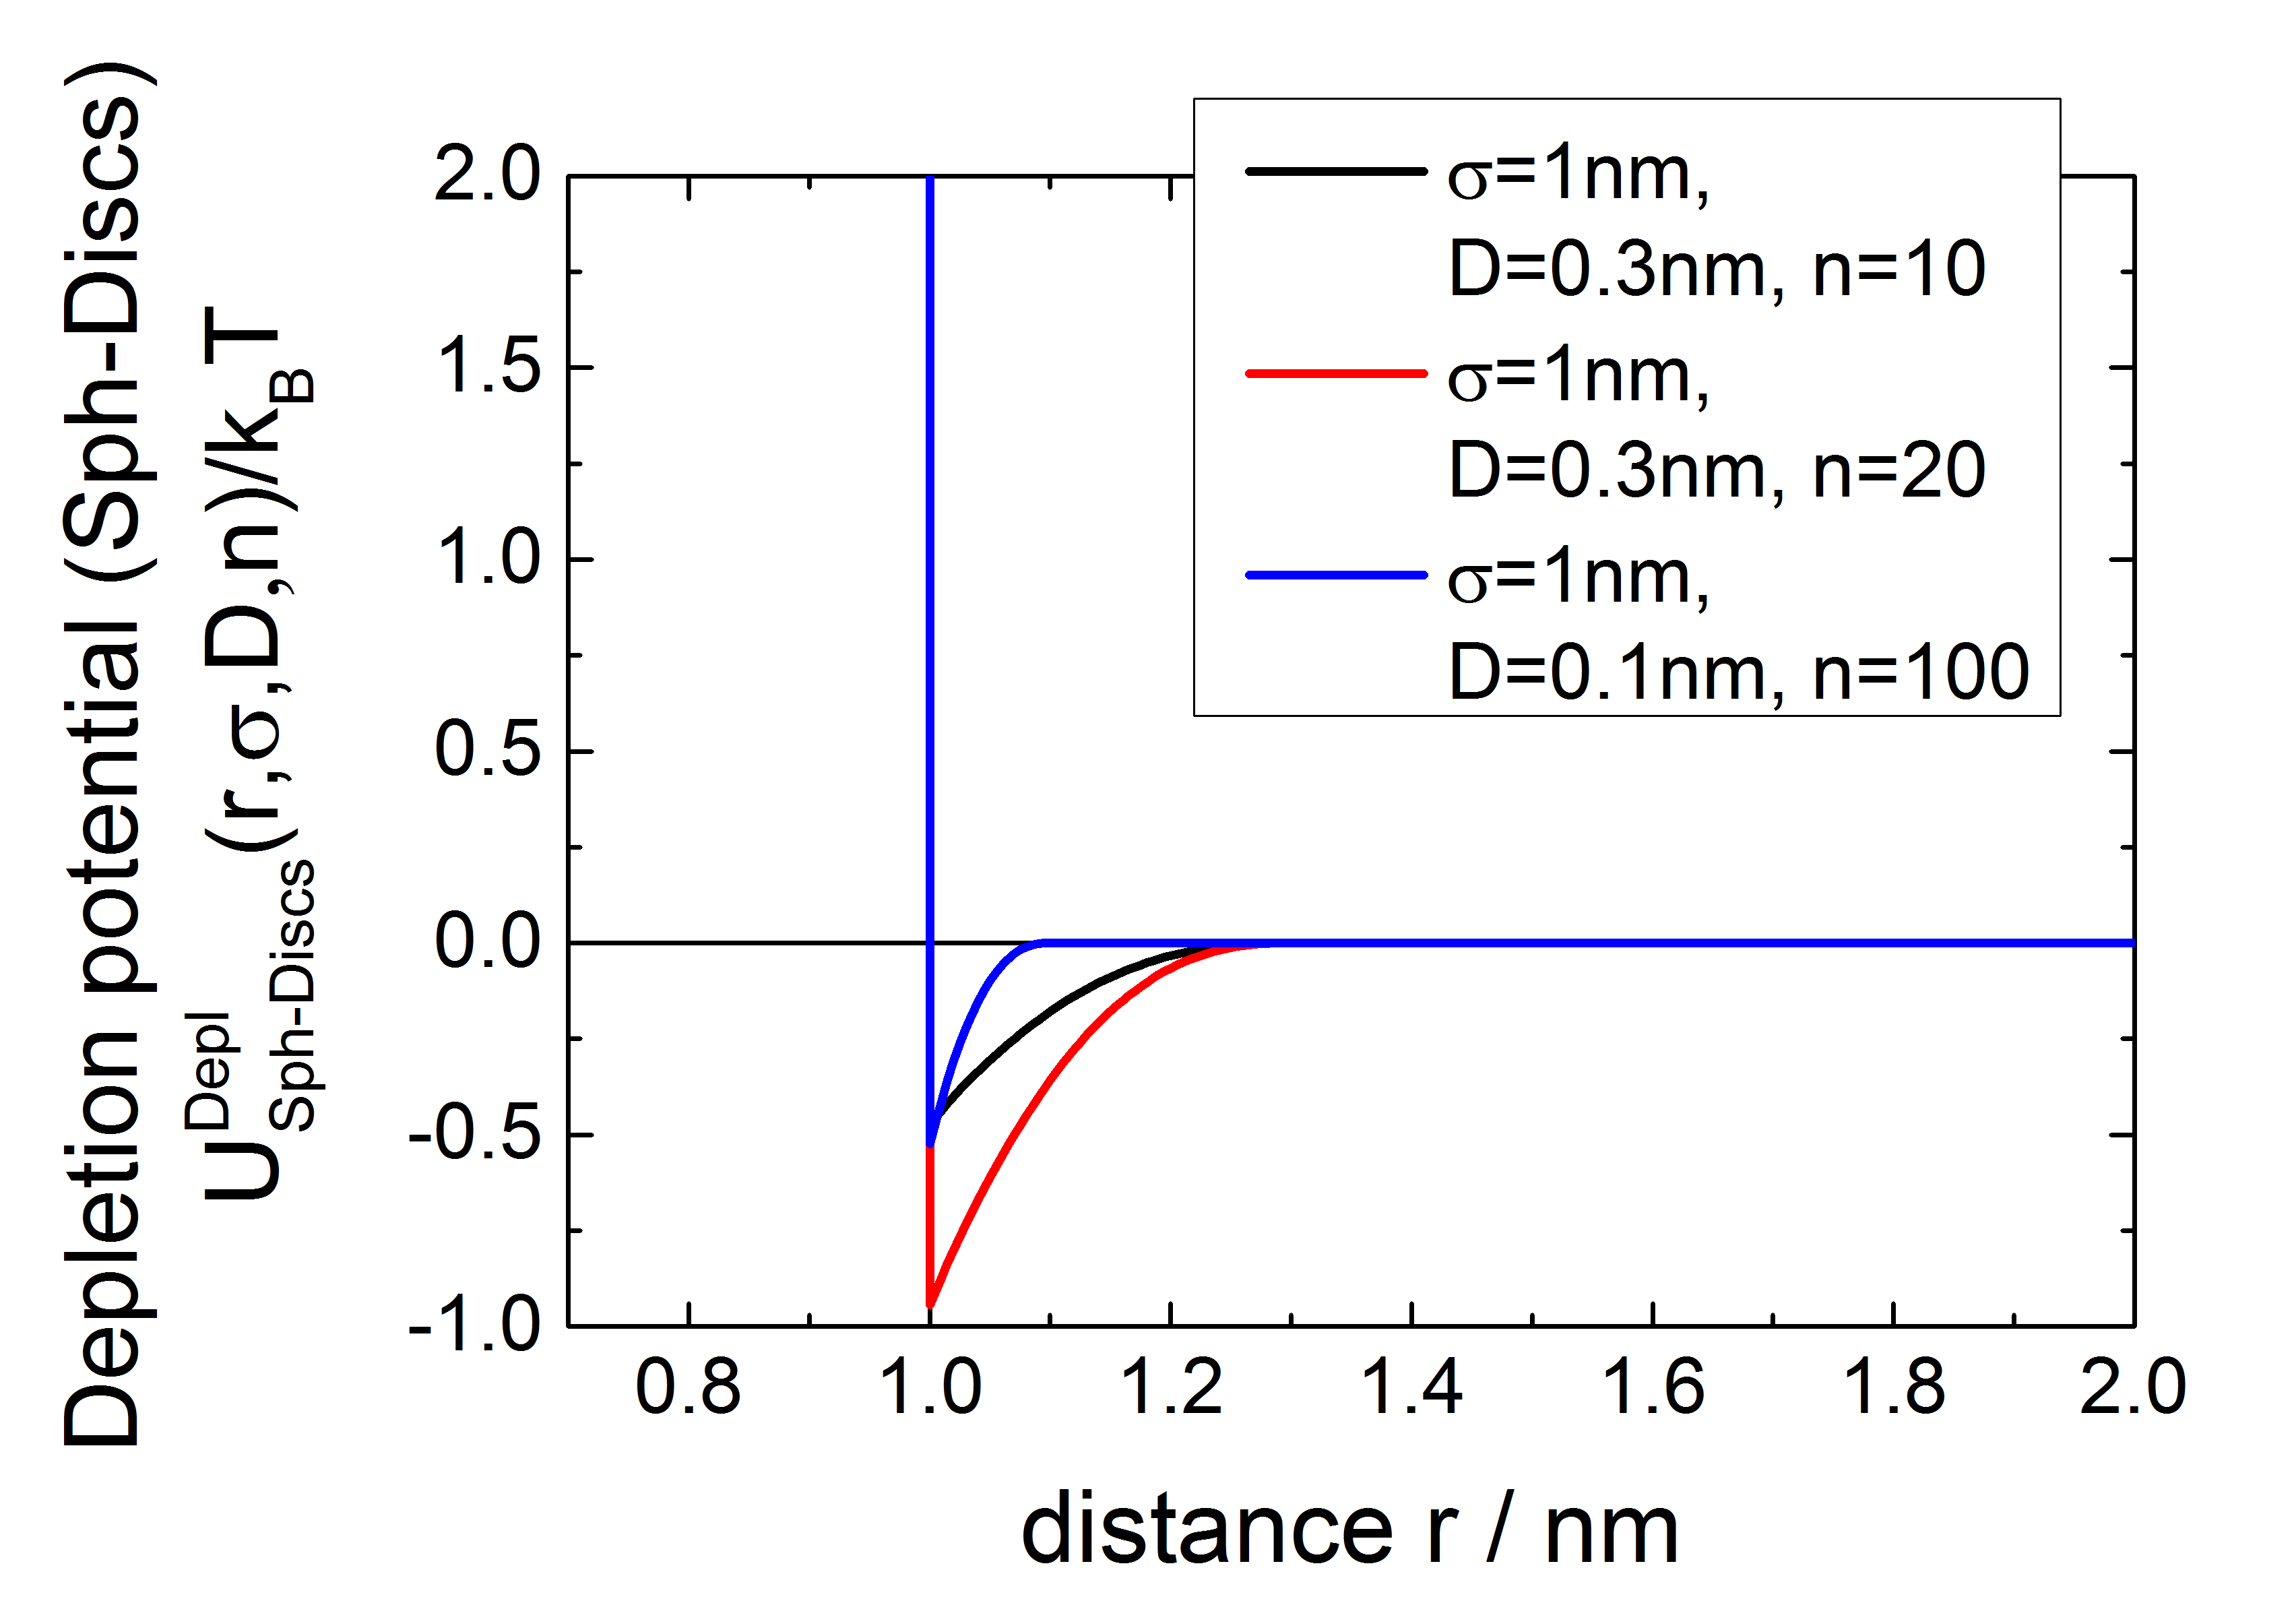
\includegraphics[width=0.45\textwidth,height=0.314\textwidth]{../images/OZsolver/potentials/potUDepl-Sph-Discs.png}}
  \quad
  \subfigure[Mayer-f function of $u^\text{depl}_\text{discs}(r,\sigma,\ldots)$]{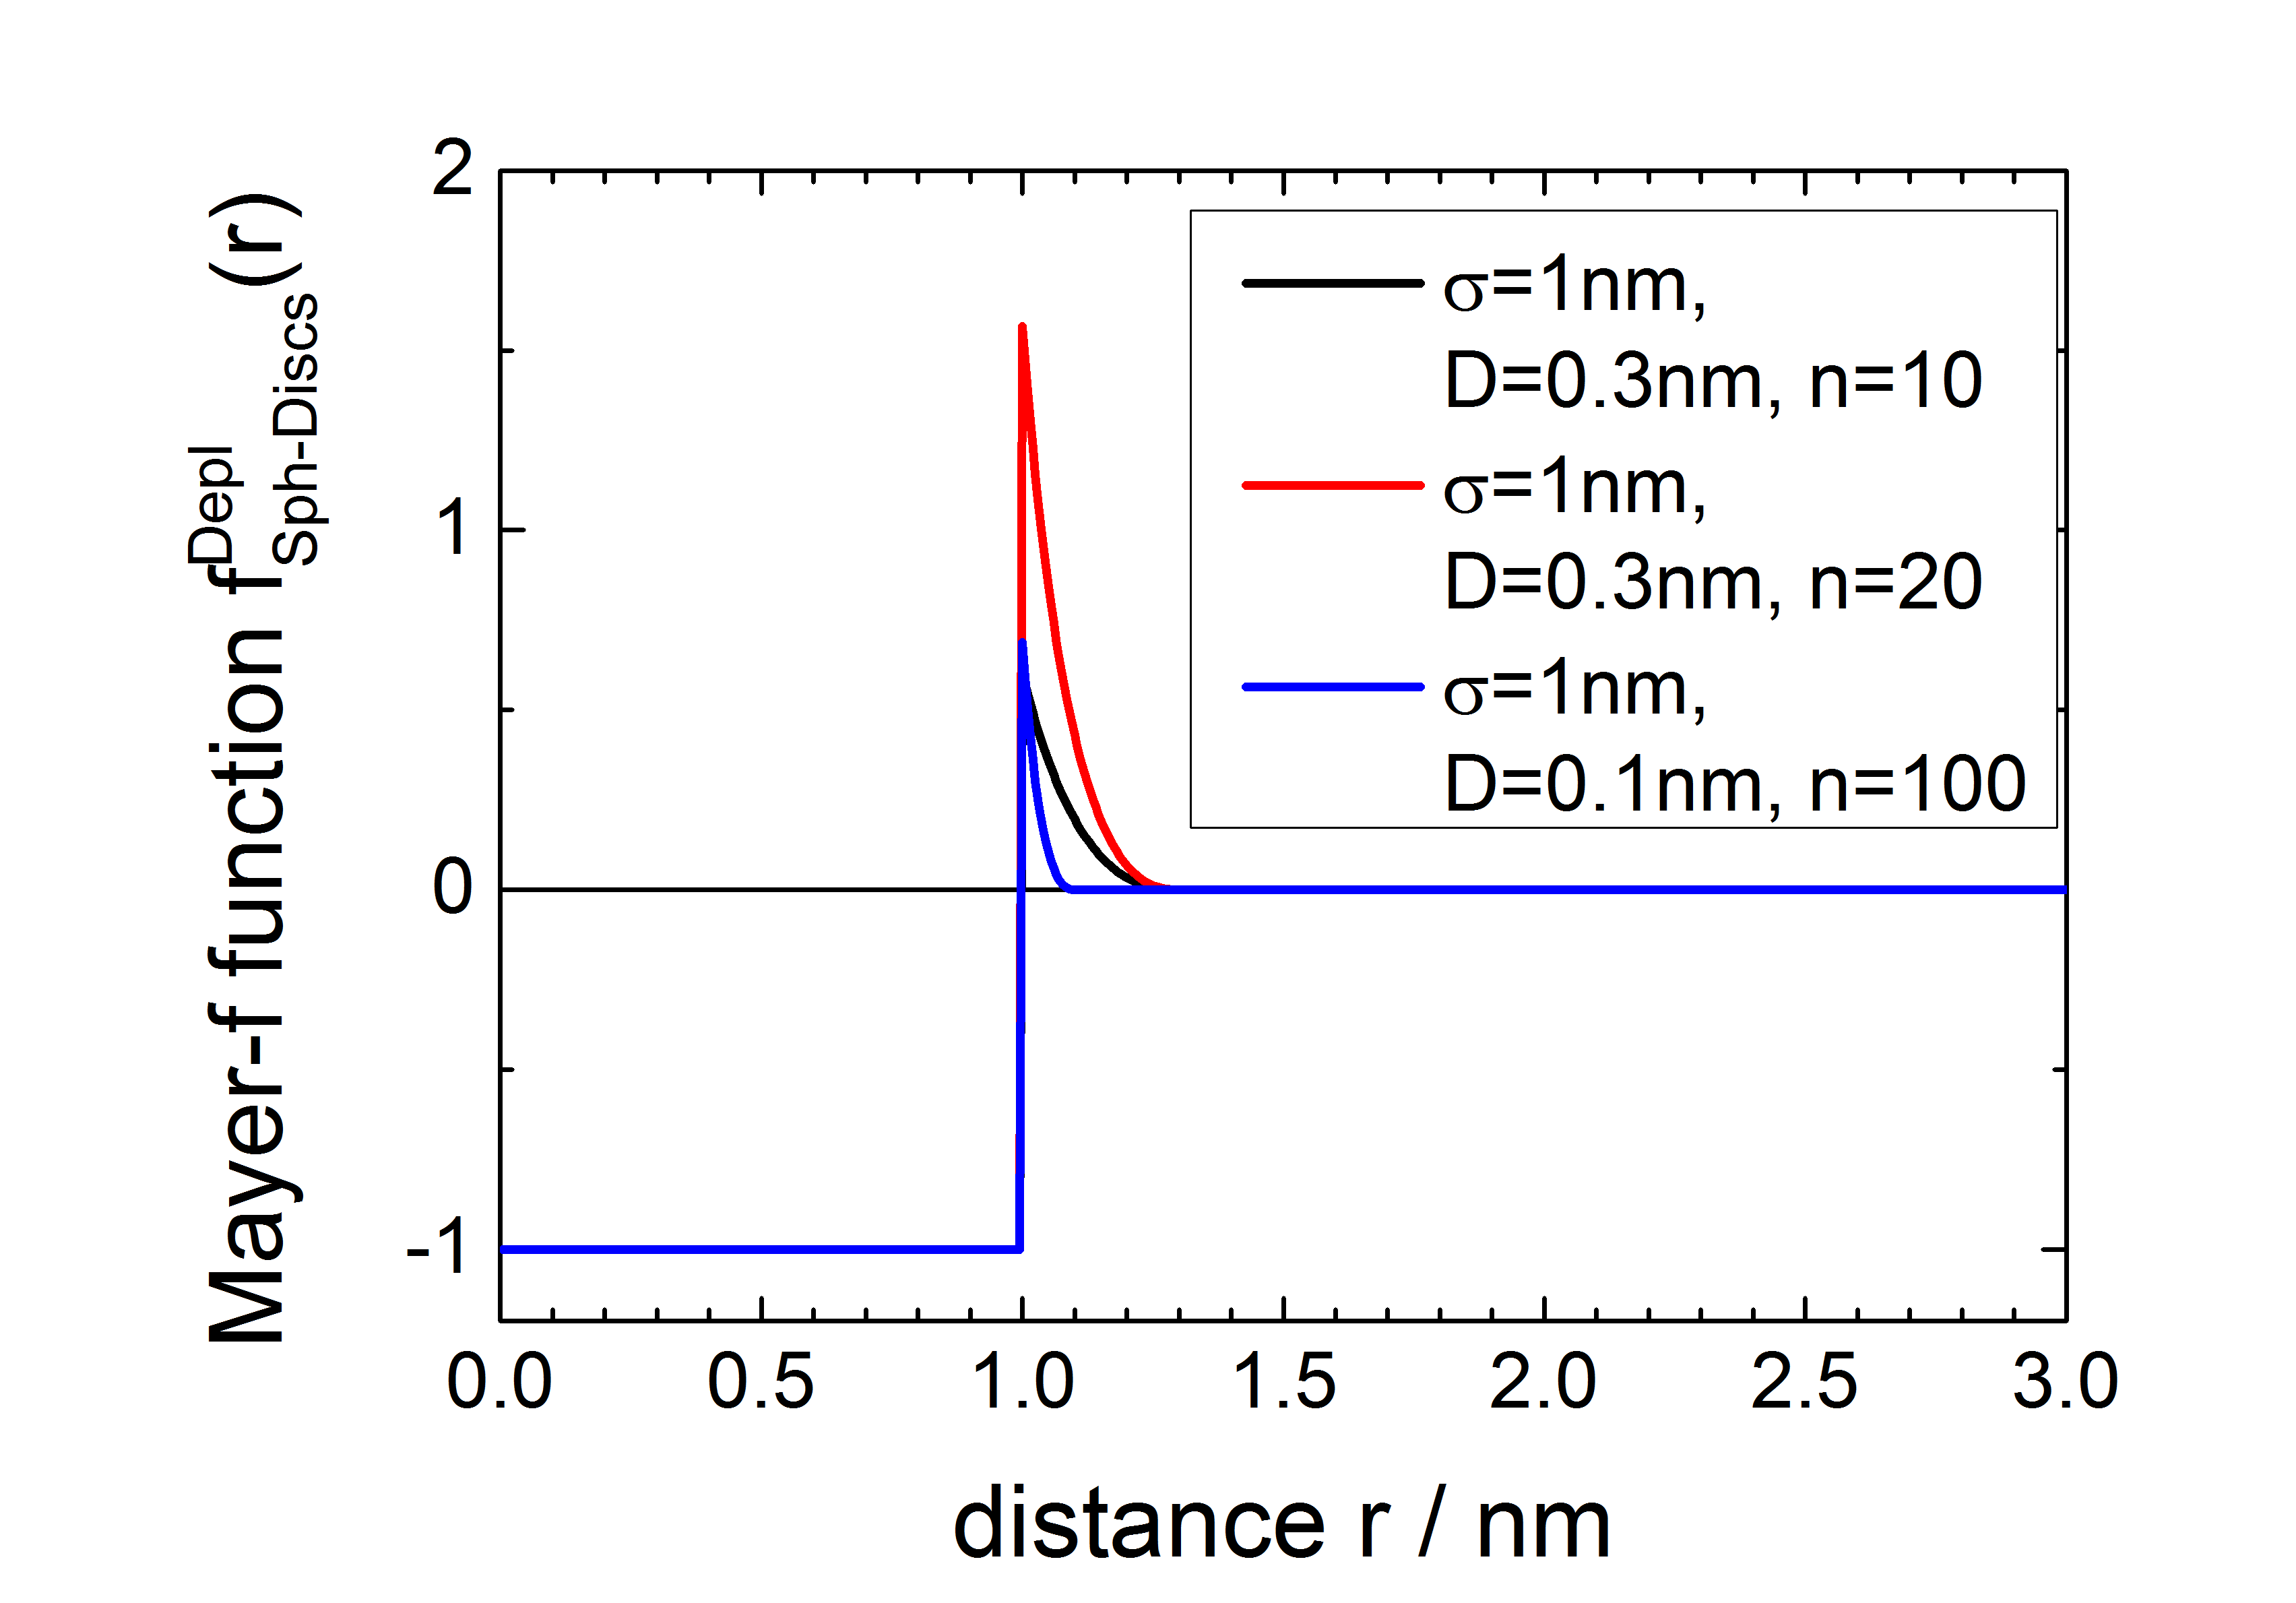
\includegraphics[width=0.45\textwidth,height=0.314\textwidth]{../images/OZsolver/potentials/potfDepl-Sph-Discs.png}}
  \caption{potential $u^\text{depl}_\text{discs}(r,\sigma,\ldots)$ and it's Mayer-f function $\exp(-u^\text{depl}_\text{discs}(r,\sigma,\ldots)/k_BT)-1$}
\end{figure}

Another depletion potential of two hard spheres of diameter $\sigma$ surrounded
by infinitely thin hard rods of length $L$ is given by
\begin{align}
u^\text{depl}_\text{rods}(r) &= -k_\text{B} T (N_\text{I}+N_\text{II}-N_\text{III}) \\
N_\text{I} &= n_d \frac{\pi}{12}\sigma L^2 \left(1-\frac{r-\sigma}{L}\right)^2
                \left(3+2\frac{L}{\sigma}+\frac{r-\sigma}{\sigma}\right)\\
\begin{split}
N_\text{II} - N_\text{III} &= \frac{\pi}{12} n_d L^2\sigma
                              \left\{ -2
                                      -\left(\frac{r-\sigma}{D}\right)^3
                                      +3\frac{r-\sigma}{D}\right\}
\end{split}
\end{align}

\begin{figure}[htb]
\centering
  \subfigure[potential between two large spheres and rodlike depleting agents $u^\text{depl}_\text{rods}(r,\sigma,\ldots)$]{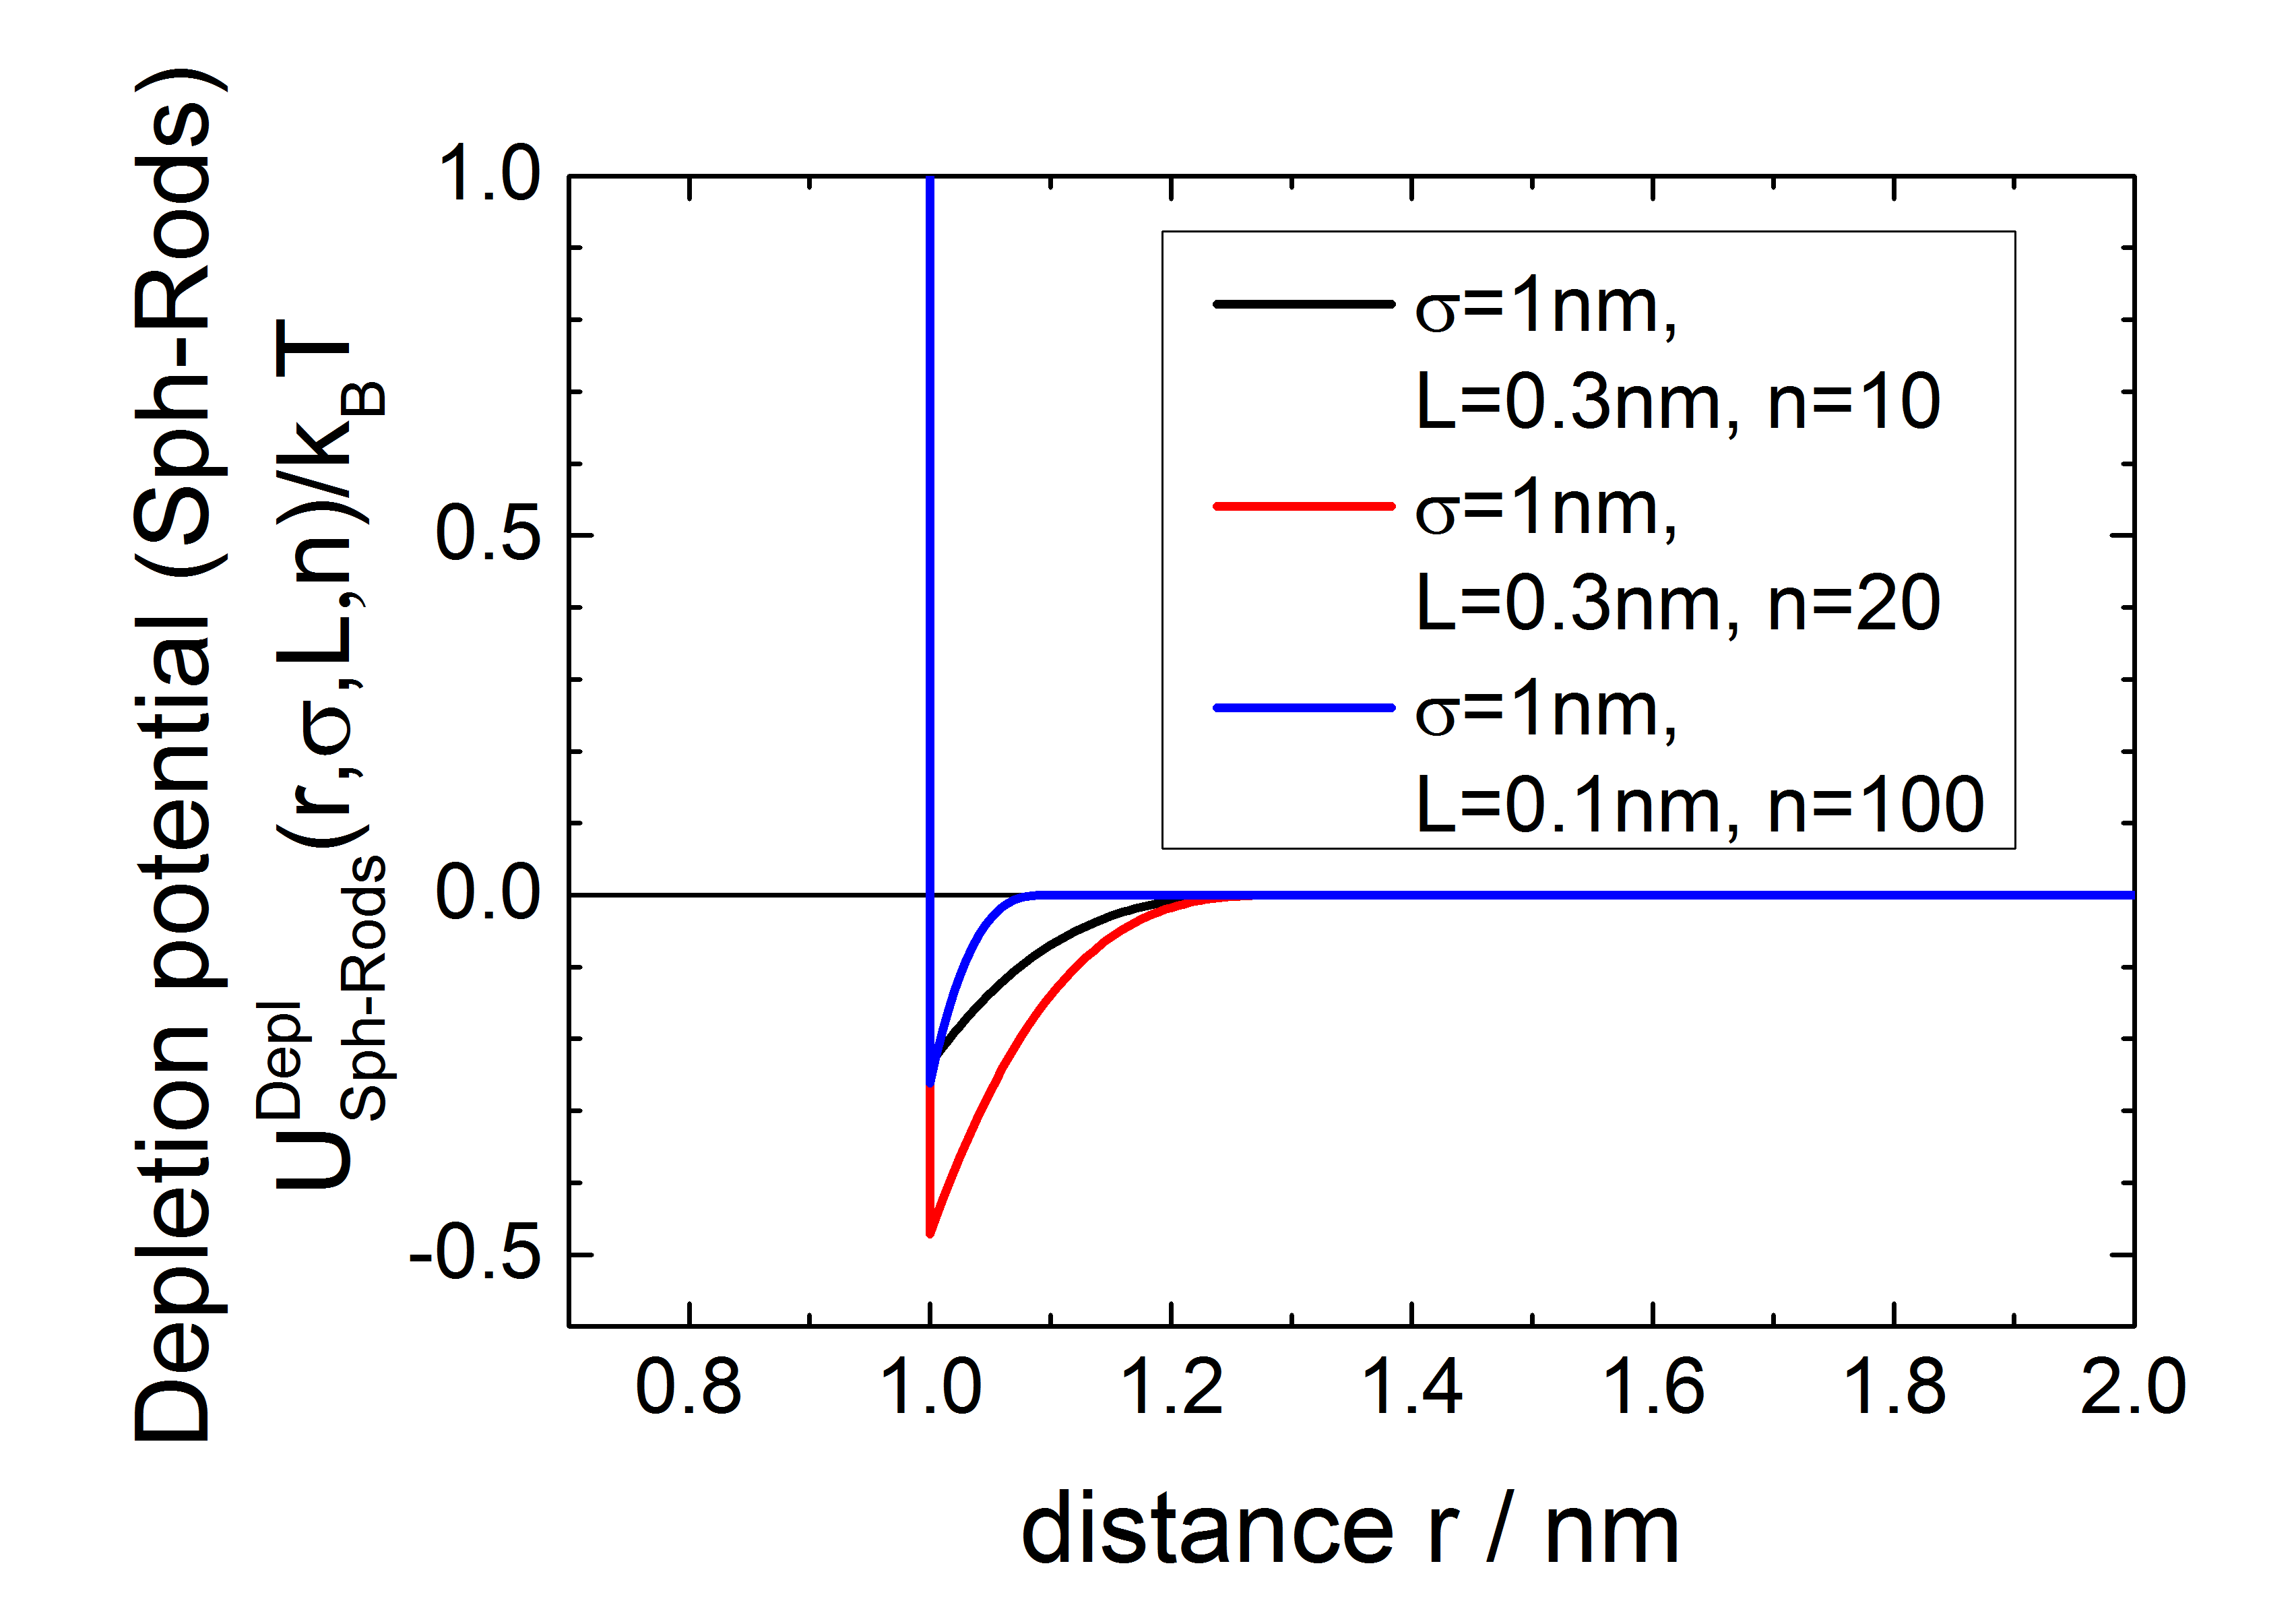
\includegraphics[width=0.45\textwidth,height=0.314\textwidth]{../images/OZsolver/potentials/potUDepl-Sph-Rods.png}}
  \quad
  \subfigure[Mayer-f function of $u^\text{depl}_\text{rods}(r,\sigma,\ldots)$]{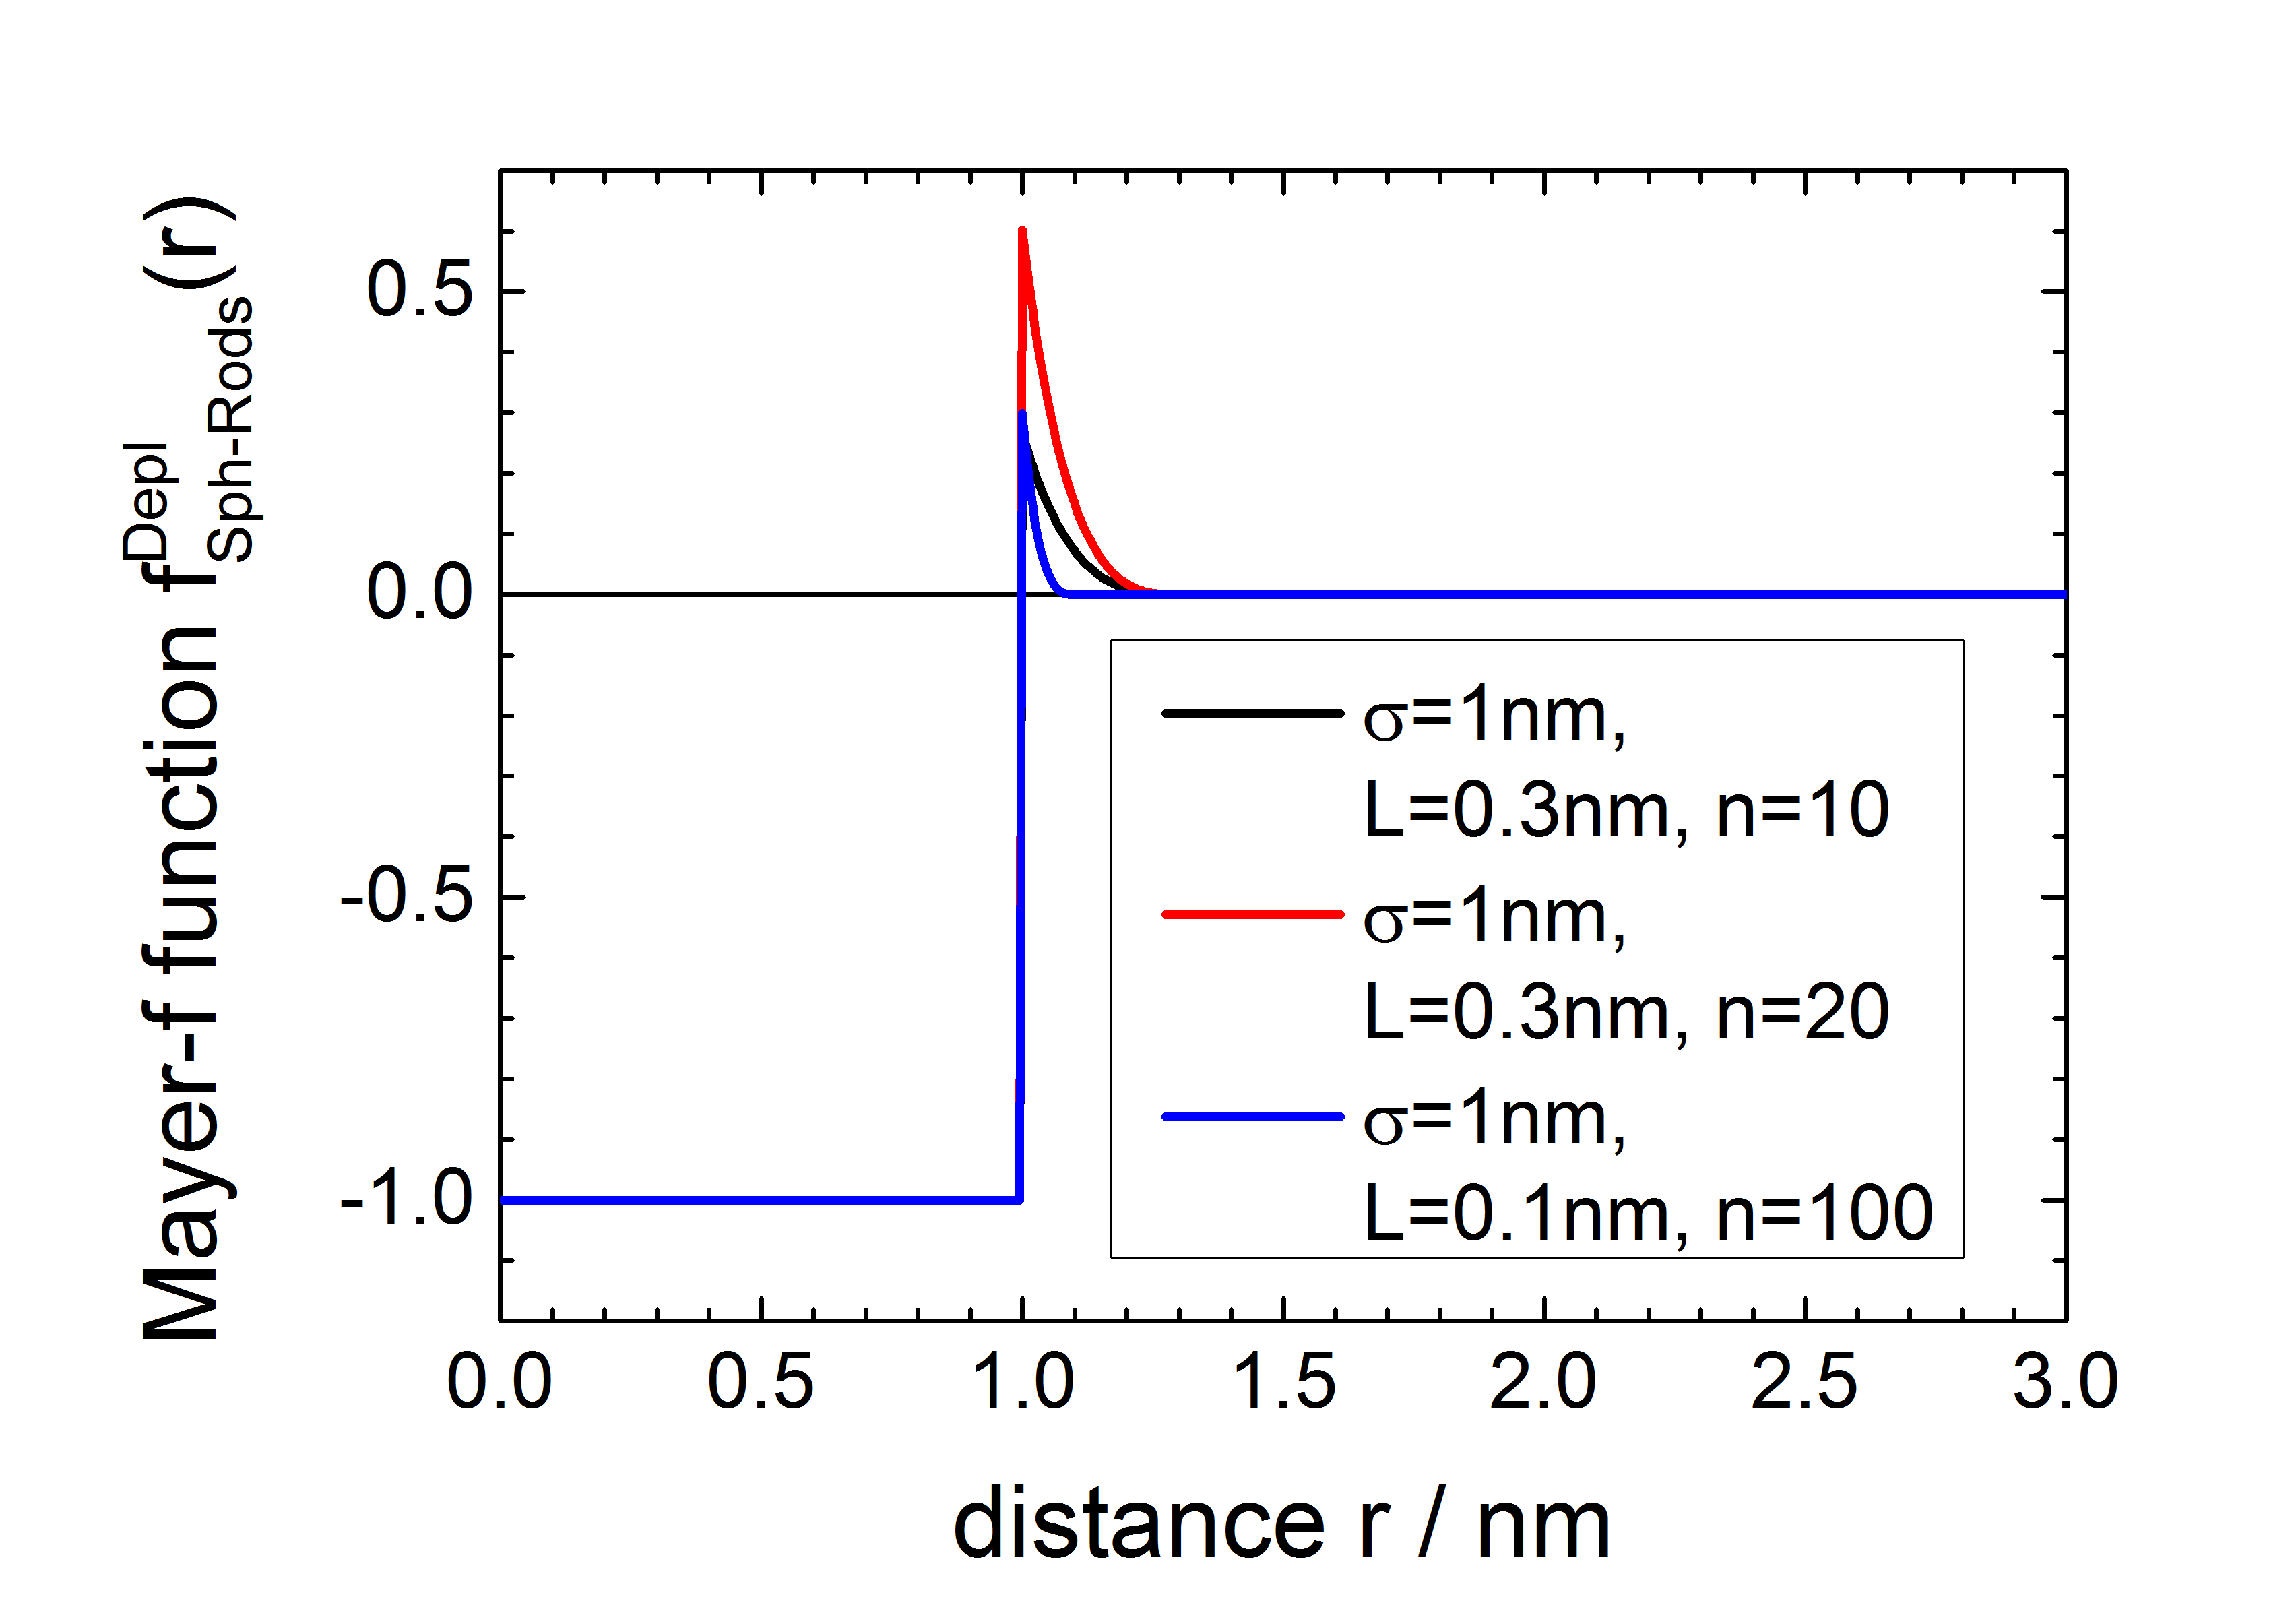
\includegraphics[width=0.45\textwidth,height=0.314\textwidth]{../images/OZsolver/potentials/potfDepl-Sph-Rods.png}}
  \caption{potential $u^\text{depl}_\text{rods}(r,\sigma,\ldots)$ and it's Mayer-f function $\exp(-u^\text{depl}_\text{rods}(r,\sigma,\ldots)/k_BT)-1$}
\end{figure}

% \vphantom{.}~\\
\newpage
\subsection{Ionic Microgel Potential}
~\\

According to \cite{Likos2011} the effective potential in ionic microgels can be partitioned in a contribution
$\Phi_{r \leq \sigma}(r)$ for the overlap region $r \leq \sigma$ and one $\Phi_{r > \sigma}(r)$ for $r>\sigma$.
\begin{align}
u^\text{im}(r) &= k_\text{B} T
\begin{cases}
\Phi_{r\leq\sigma}(r)   & \mbox{for } r \leq \sigma \\
\Phi_{r>\sigma}(r)      & \mbox{for } r > \sigma
\end{cases}
\end{align}
For the overlapping particle it has the form
\begin{align}
\Phi_{r\leq\sigma}(r) &= \frac{2Z^2\text{e}^2}{\epsilon\sigma}
                         \left[\frac{6}{5}-2\left(\frac{r}{\sigma}\right)^2
                                          +\frac{3}{2}\left(\frac{r}{\sigma}\right)^3
                                          -\frac{1}{5}\left(\frac{r}{\sigma}\right)^5
                         \right]
                        - \frac{72 Z^2e^2}{\epsilon\kappa^4\sigma^4r}\Phi_\text{ind}(r)
\end{align}
where $\Phi_\text{ind}(r)$ is given by the expression
\begin{align}
\begin{split}
  \Phi_\text{ind}(r) =&  \left(1-\text{e}^{-\kappa r}+\frac{1}{2}\kappa^2r^2+\frac{1}{24}\kappa^4r^4\right)
                        \left(1-\frac{4}{\kappa^2\sigma^2}\right) \\
                     & +\frac{4}{\kappa\sigma}\text{e}^{-\kappa\sigma}\sinh\left(\kappa r\right)\\
                     & +\left[\text{e}^{-\kappa\sigma}\sinh\left(\kappa\sigma\right)
                                    +\kappa^2\sigma r
                                    +\frac{1}{6}\kappa^4\left(\sigma^3 r + r^3 \sigma \right)
                        \right] \left(1+\frac{4}{\kappa^2\sigma^2}\right)\\
                     & -\frac{4r}{\sigma} \left(1+\frac{1}{2}\kappa^2\sigma^2+\frac{1}{30}\kappa^4\sigma^4\right) \\
                     & -\frac{8r^3}{3\sigma^3}\left(\frac{\kappa^2\sigma^2}{4}+\frac{\kappa^4\sigma^4}{12}\right)
                       -\frac{1}{180}\frac{\kappa^4}{\sigma^2} r^6
\end{split}
\end{align}
For the nonoverlapping distances the effective potential becomes
\begin{align}
\Phi_{r>\sigma}(r) &= \frac{144Z^2e^2}{\epsilon\kappa^4\sigma^4}
                      \left[\cosh\left(\kappa\sigma/2\right)-\frac{2\sinh\left(\kappa\sigma/2\right)}{\kappa\sigma}\right]^2
                      \frac{\text{e}^{-\kappa r}}{r}
\end{align}

% \vphantom{.}~\\
\newpage
\subsection{DLVO Potential}
~\\

For the past half century or so, the stability of charged
colloidal systems has generally been described in terms of the
DLVO (Derjaguin-Landau-Verwey-Overbeek) potential between
two colloidal particles. The DLVO potential is composed
of a long-range screened Coulomb repulsion part $u^\text{el}(r)$
and a short-range van der Waals attraction part $u^\text{vdW}(r)$
\cite{Naegele1996}.
\begin{align}
u^\text{DLVO}(r) &=
\begin{cases}
\infty                          & \mbox{if } r \leq \sigma \\
u^\text{vdW}(r)+u^\text{el}(r)  & \mbox{if } r >    \sigma
\end{cases}
\end{align}
with
\begin{align}
u^\text{vdW}(r) &= -k_\text{B} T \frac{A_\text{H}}{12} \left(
                  \frac{\sigma^2}{\left(r^2-\sigma^2\right)}
                + \left(\frac{\sigma}{r}\right)^2
                + 2\ln\left(1-\left(\frac{\sigma}{r}\right)^2\right)
                \right) \\
u^\text{el}(r)  &= k_\text{B} T L_B Z_\text{eff}^2
                \frac{1}{\left(1+\kappa\sigma/2\right)^2}
                \frac{\exp\left(-\kappa (r-\sigma)\right)}{r}
\end{align}
$A_\text{H}$ is the Hamaker constant. $L_B=\frac{e^2}{4\pi \epsilon_r \epsilon_0 k_\text{B} T }$
is the so-called Bjerrum length\footnote{In Gaussian units, $4\pi\varepsilon_0 = 1$ and the Bjerrum
length has the simpler form $L_B = \frac{e^2}{\varepsilon_r k_B T}$.}. The vacuum permittivity is
$\epsilon_0= 8.854 187 817 \times 10^{-12} \left[\frac{\text{F}}{\text{m}}\right]$ and the elementary
electric charge $e=1.602176565(35)\times 10^{-19}$coulombs\footnote{The Gaussian units use
the statcoulomb (statC) instead. The conversion between C and statC is different in different contexts.
In case of electric charges $1\text{C} = 2997924580 \text{ statC} \approx 3.00\times 10^9 \text{ statC}$.}.
For water at 278 K with a relativ permittivity of $\epsilon_r=78.7$ the Bjerrum length is $L_B=0.713$nm.
The effective macroion valency is denoted $Z_\text{eff}$, and $\kappa^{-1}$ is the Debye-H\"uckel screening length
due to all macroions. This length characterize the typical distance at which the charge at the origin is screened
by the other charges. It is given by $\kappa^{2}= 4\pi L_B \sum_{i=1}^N n_i Z_i$, where $n_i$ is the number density
of ion $i$, $Z_i$ is the charge number of that ion, and the sum is taken over all ions in the
solution. A discussion about effective parameters can be found in \cite{Alexander1984,Ulander2001}.

\begin{figure}[htb]
\centering
  \subfigure[DLVO potential (Derjaguin and Landau, Verwey and Overbeek) $u^\text{DLVO}(r,\sigma,\ldots)$]{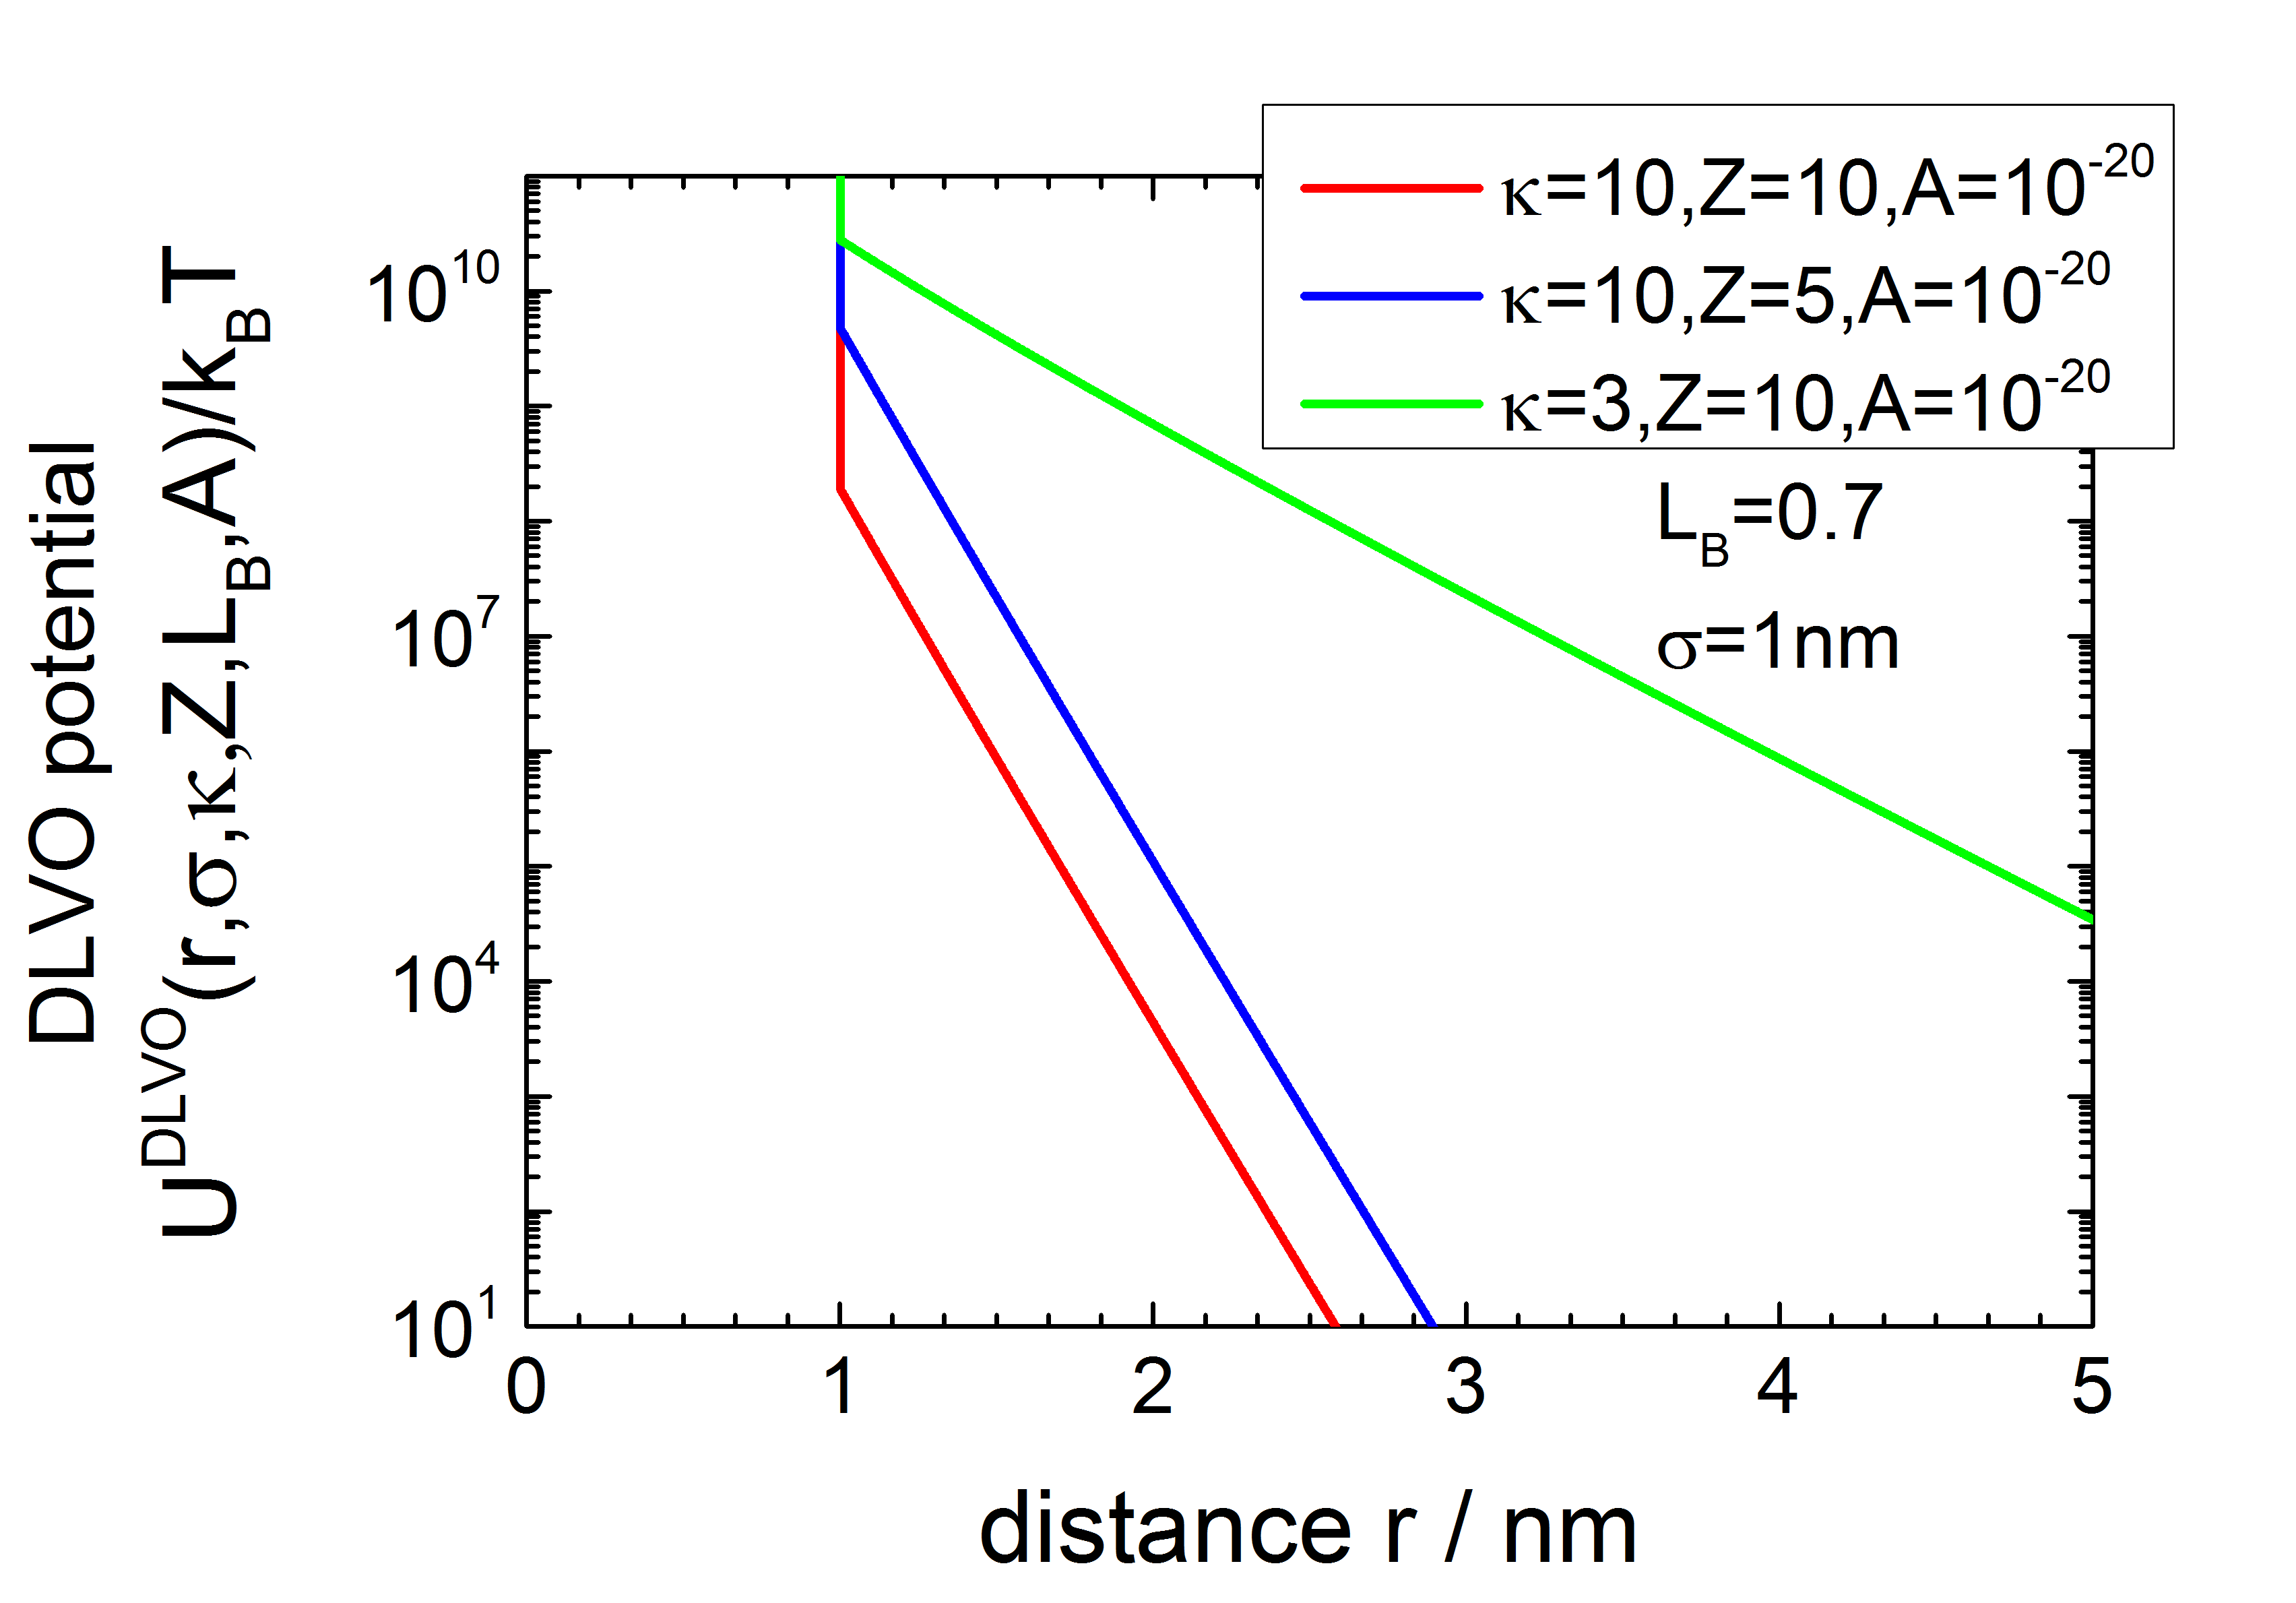
\includegraphics[width=0.45\textwidth,height=0.314\textwidth]{../images/OZsolver/potentials/potUDLVO_a.png}}
  \quad
  \subfigure[Mayer-f function of $u^\text{DLVO}(r,\sigma,\ldots)$]{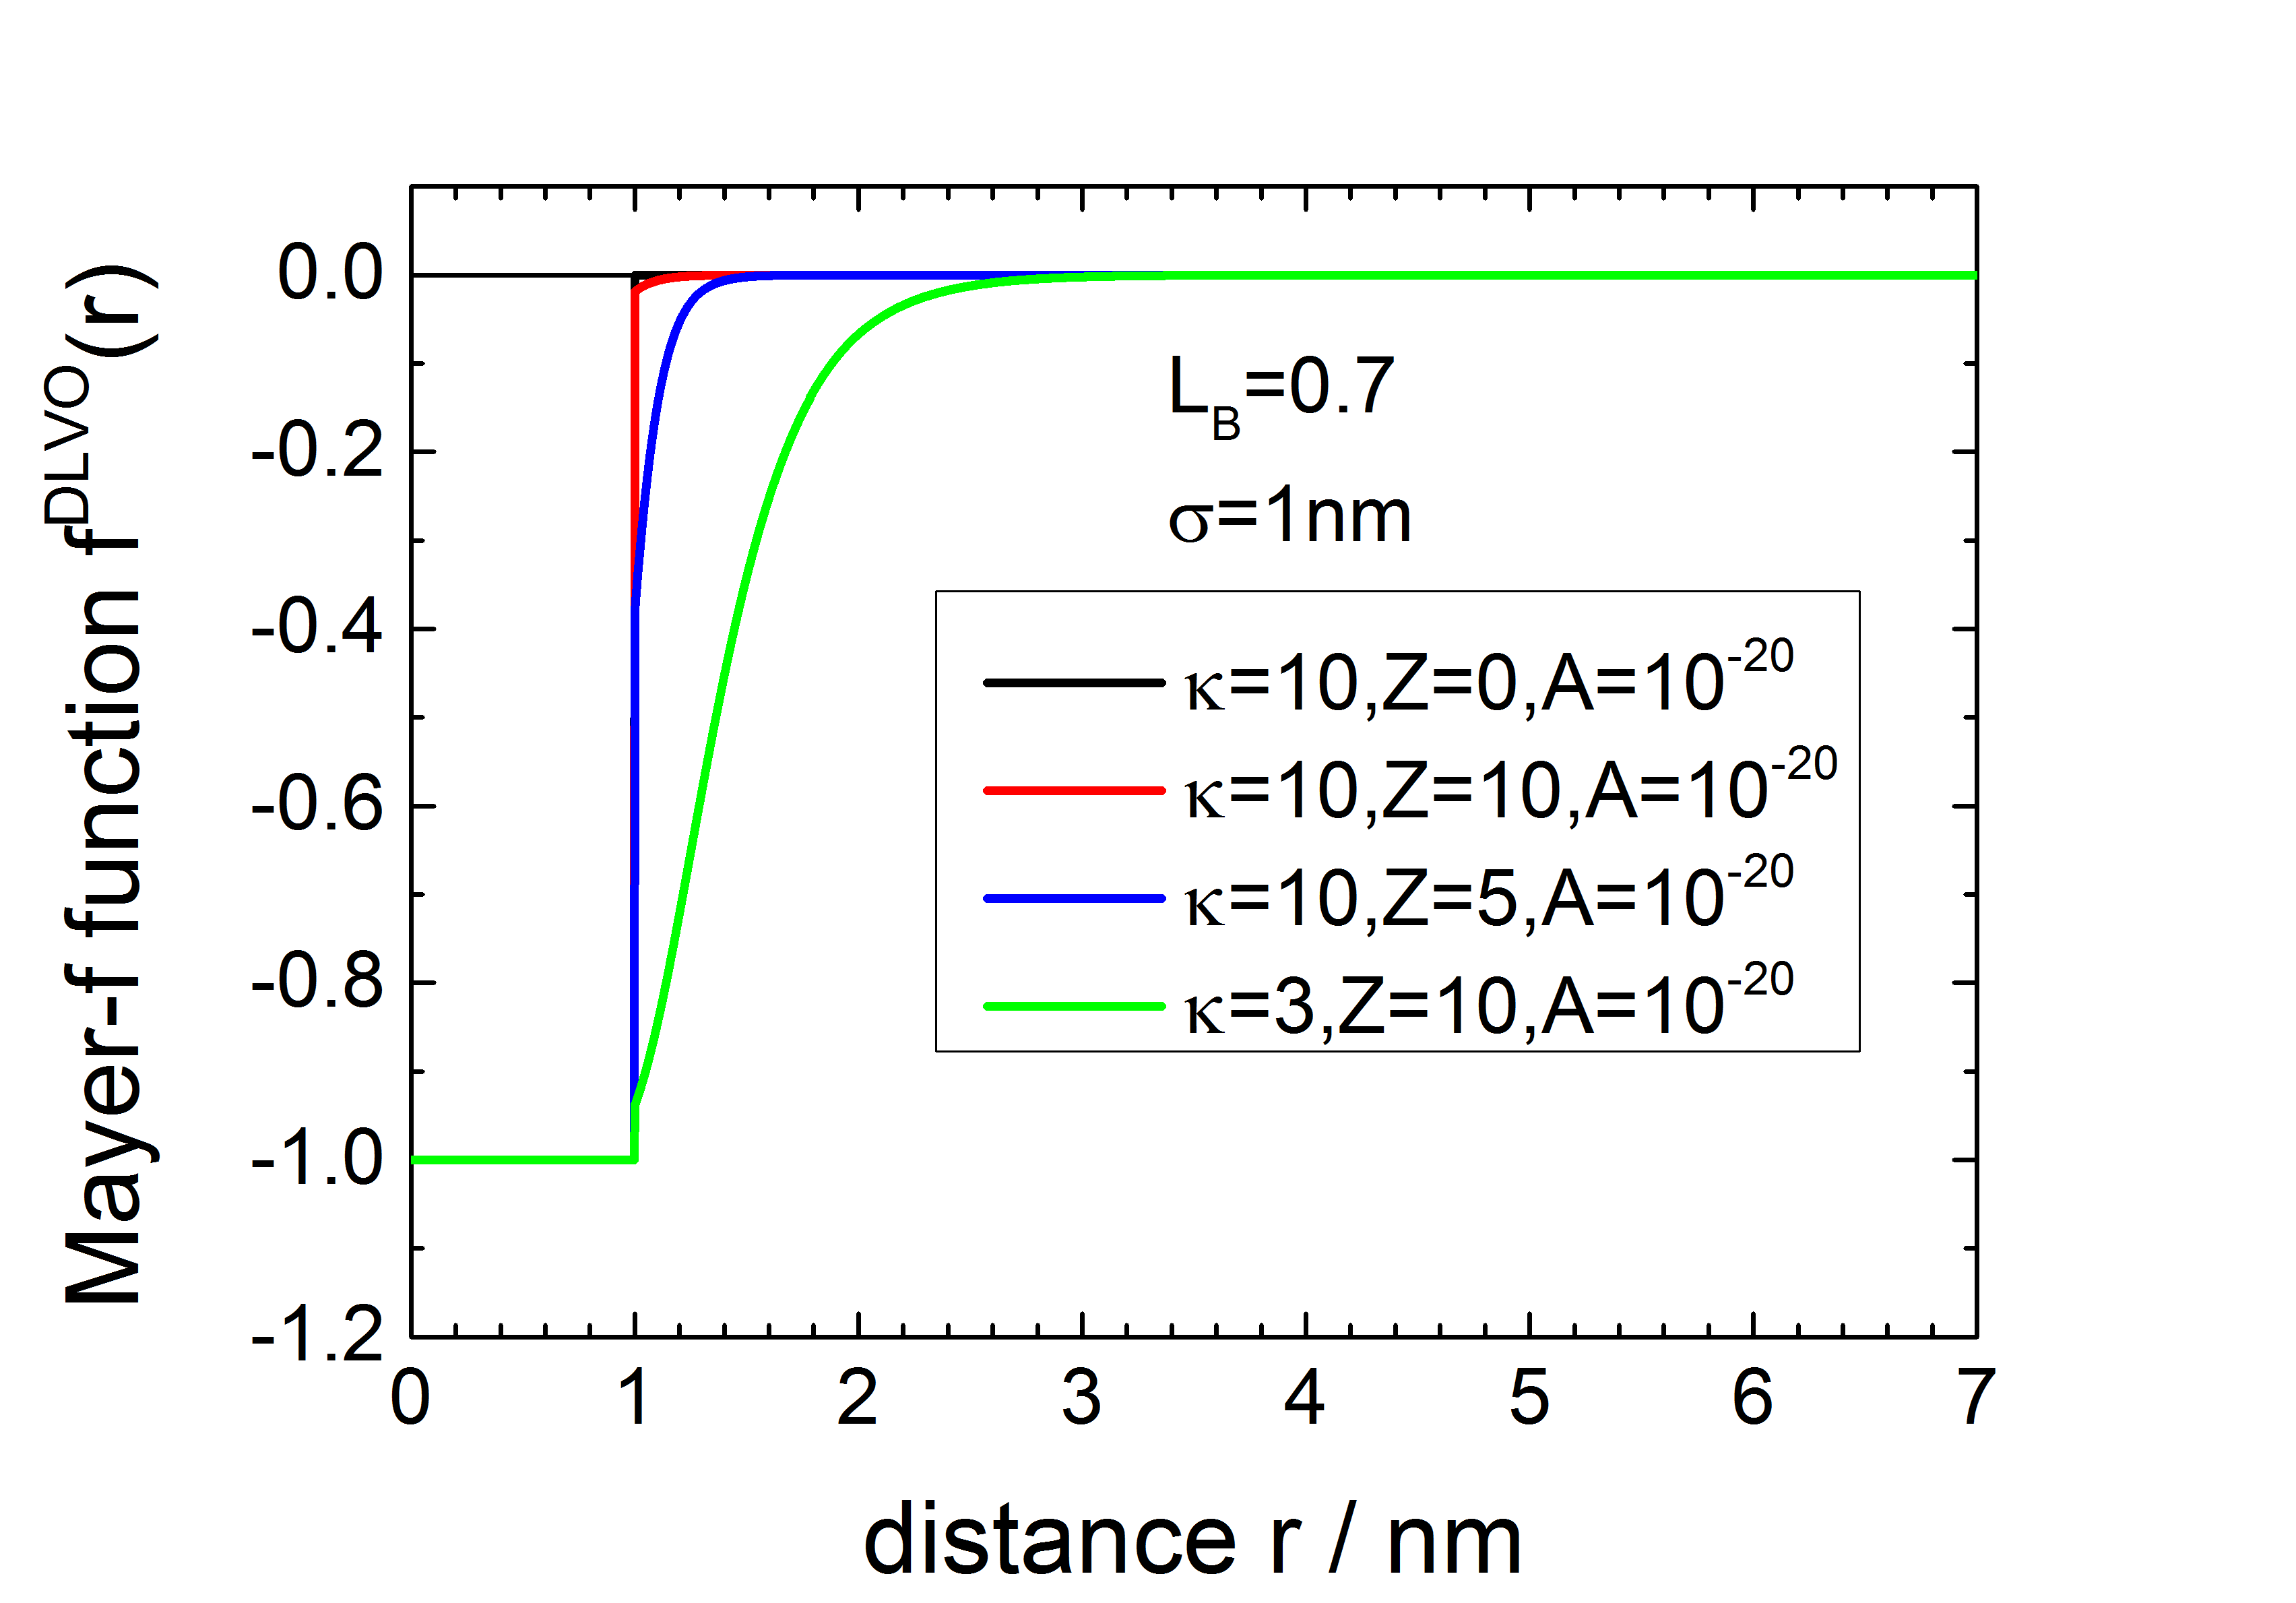
\includegraphics[width=0.45\textwidth,height=0.314\textwidth]{../images/OZsolver/potentials/potfDLVO.png}}
  \caption{potential $u^\text{DLVO}(r,\sigma,\ldots)$ and it's Mayer-f function $\exp(-u^\text{DLVO}(r,\sigma,\ldots)/k_BT)-1$}
\end{figure}

% \vphantom{.}~\\
\newpage
\subsection{Hard Core Yukawa Potential}
~\\

This potential is useful for systems with complicated potentials. Next to the hard core repulsion three
Yukawa contributions are allowed. The potential reads
\begin{align}
u^\text{HC3Y}(r,\ldots) &=
\begin{cases}
\infty                                                                  & \mbox{for } r<   \sigma \\
k_\text{B} T
\displaystyle \sum_{i=1}^{N=3} K_i\exp\left(-\lambda_i(r-\sigma)\right)& \mbox{for } r >= \sigma
\end{cases}
\end{align}
The sign of $K_i$ defines, if the potential is
repulsive ($K_i>0$) or attractive ($K_i<0$) and the modulus of $\abs{K_i}$ defines the strength of the interaction. $\lambda_i$ defines the range of the interaction and should be always a positive number.

\begin{figure}[htb]
\centering
  \subfigure[Hard Core Yukawa potential with three linear combinations of Yukawa tails $u^\text{HC3Y}(r,\sigma,\ldots)$]{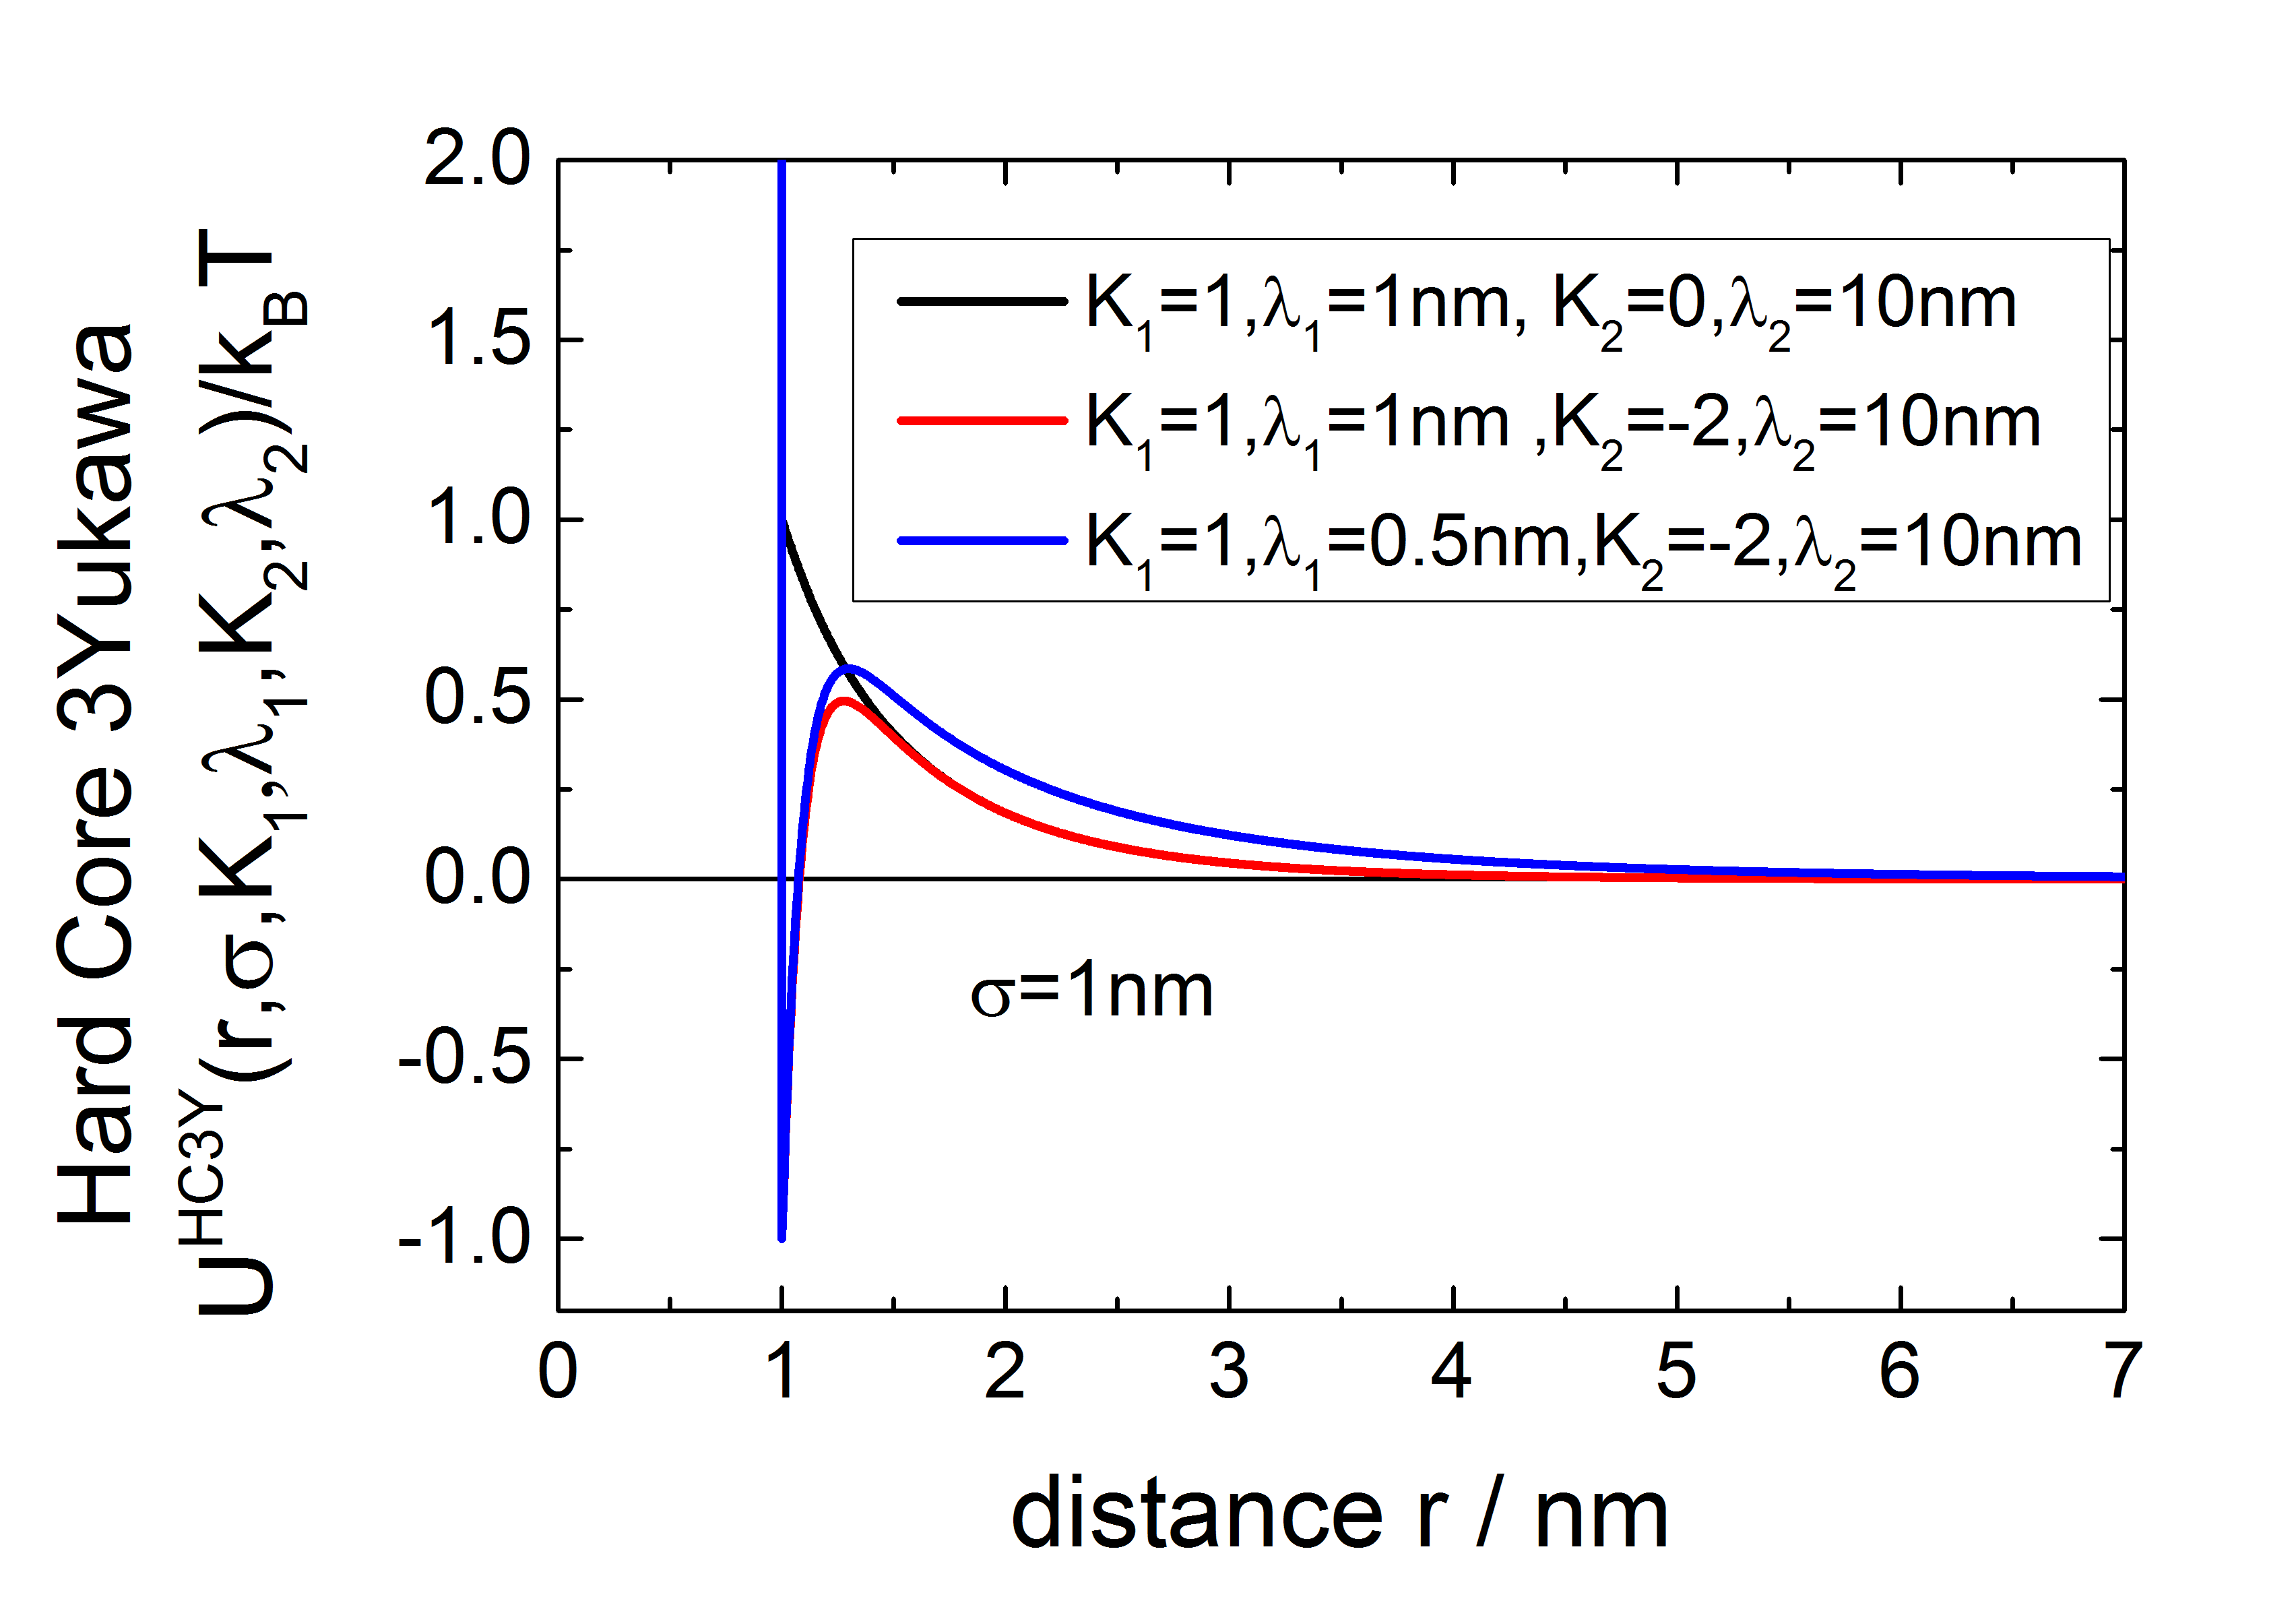
\includegraphics[width=0.45\textwidth,height=0.314\textwidth]{../images/OZsolver/potentials/potUHC3Yukawa.png}}
  \quad
  \subfigure[Mayer-f function of $u^\text{HC3Y}(r,\sigma,\ldots)$]{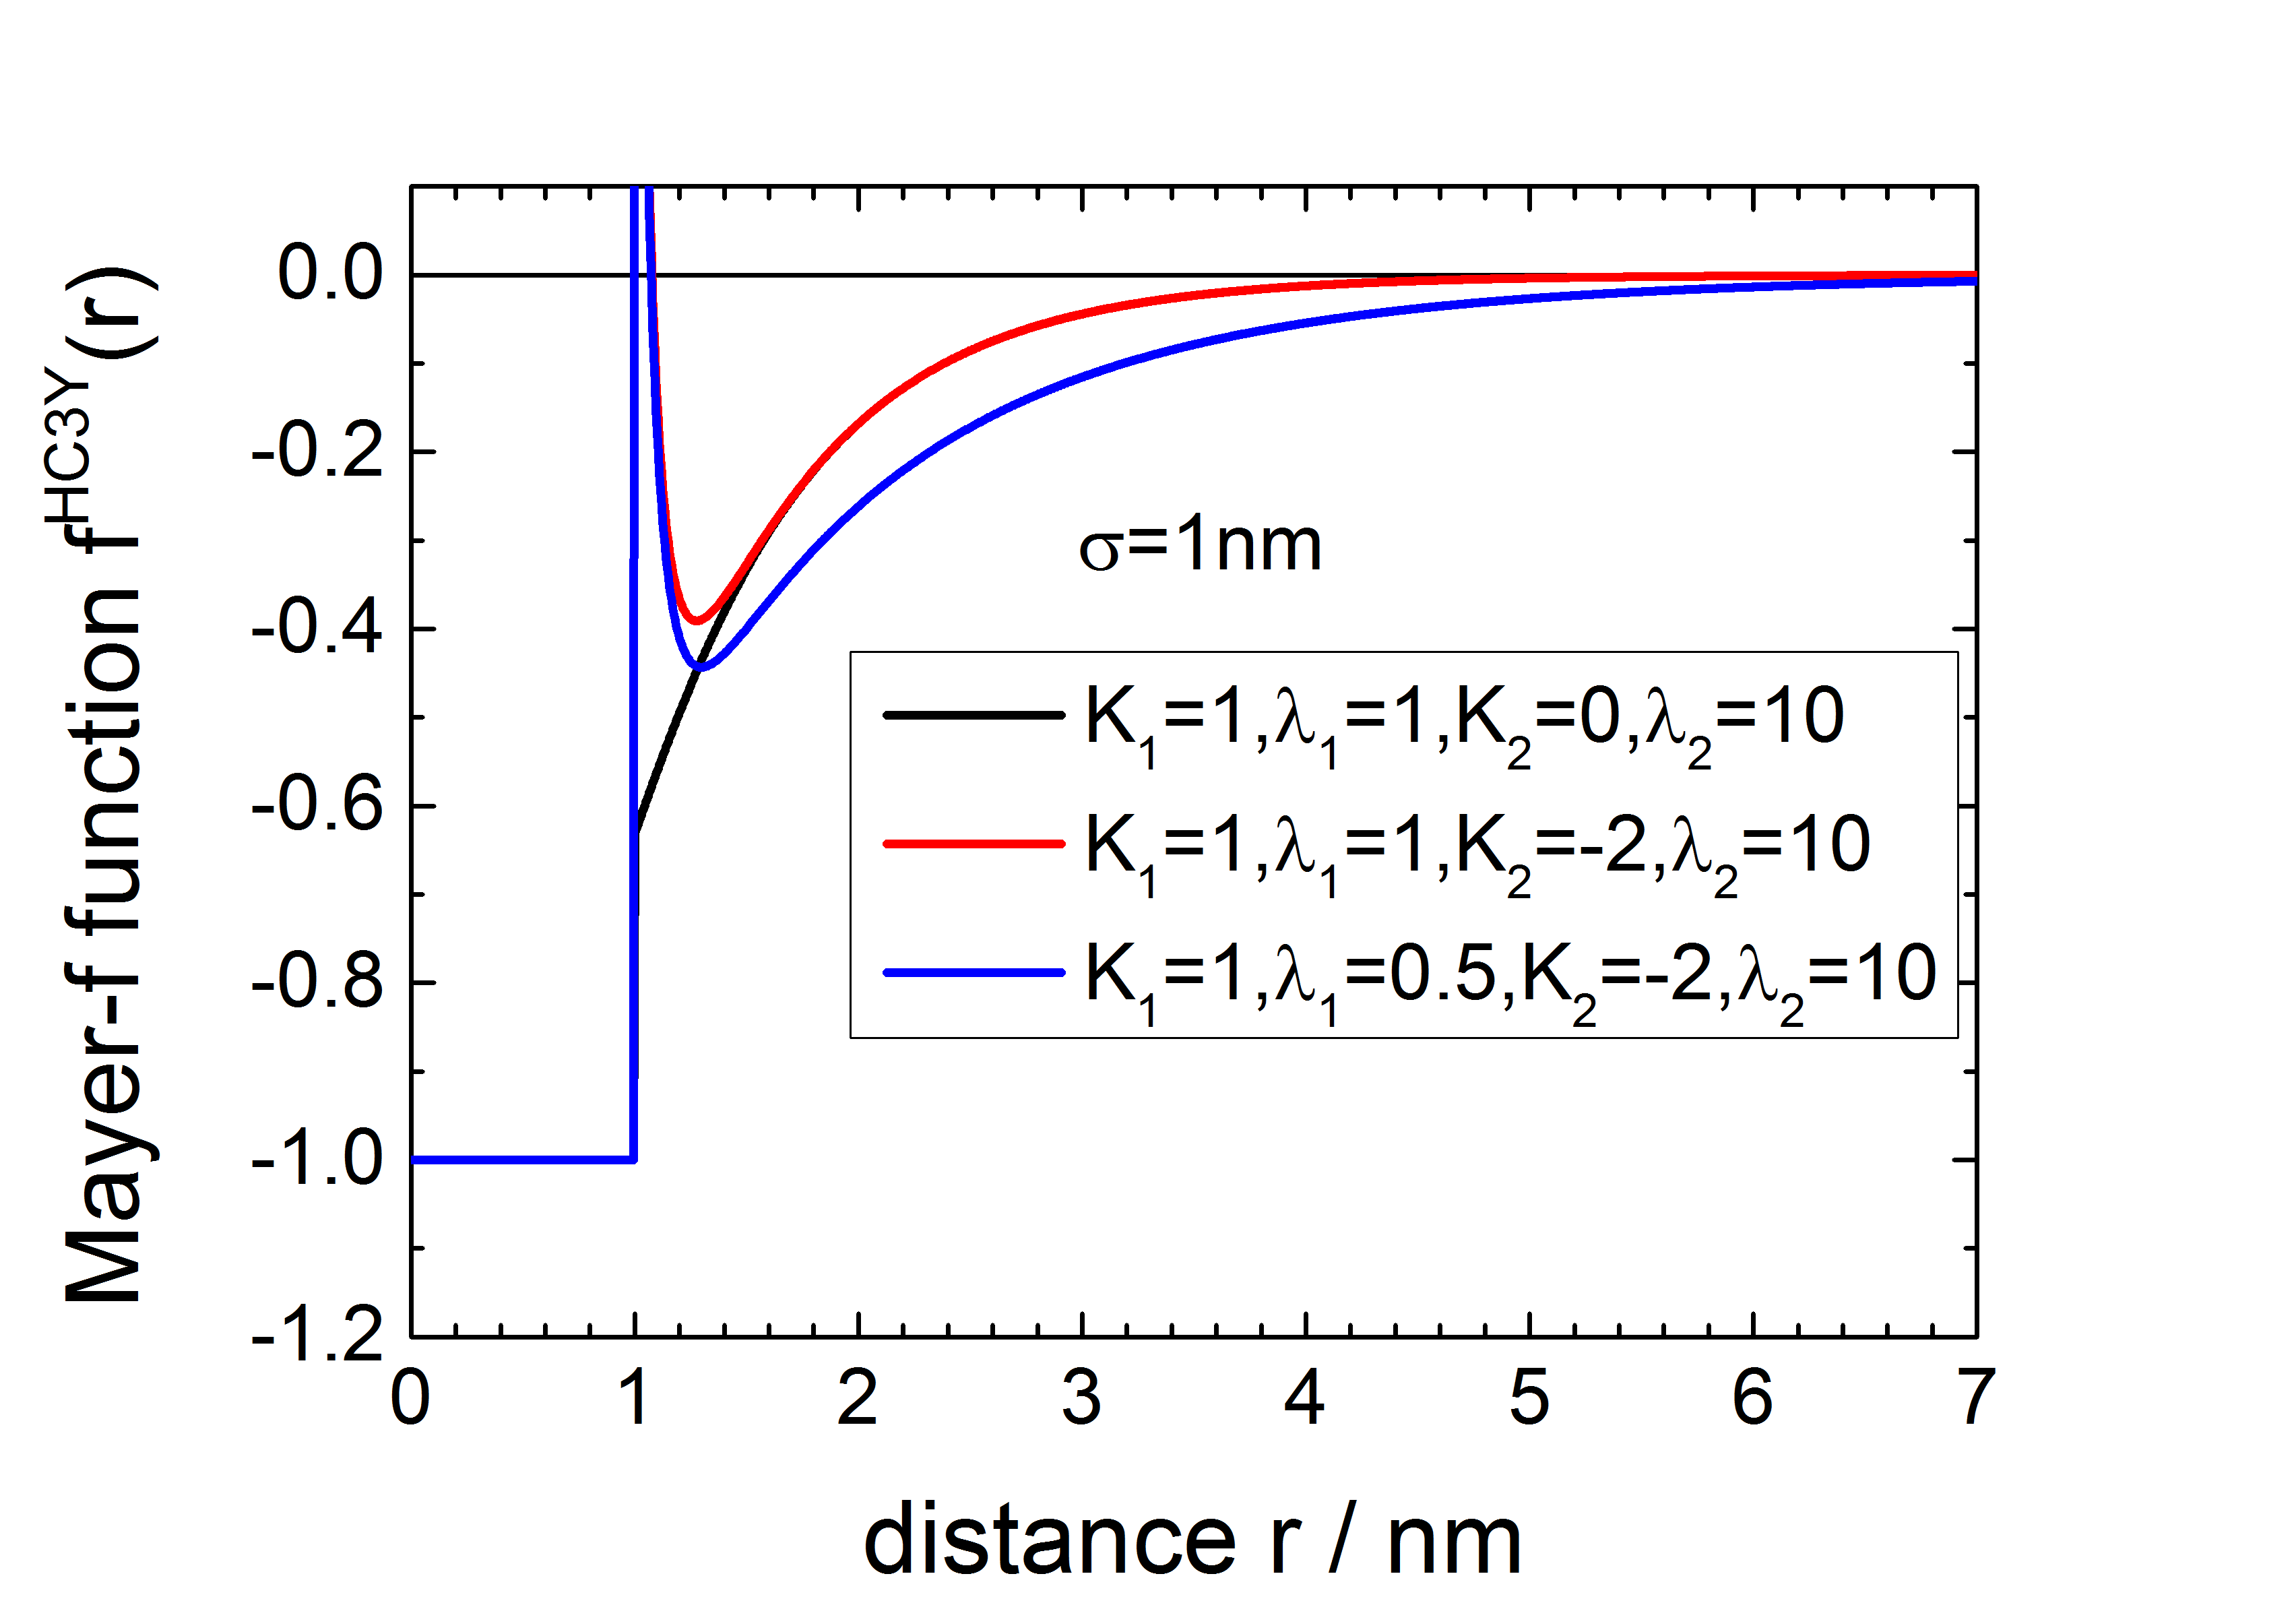
\includegraphics[width=0.45\textwidth,height=0.314\textwidth]{../images/OZsolver/potentials/potfHC3Yukawa.png}}
  \caption{potential $u^\text{HC3Y}(r,\sigma,\ldots)$ and it's Mayer-f function $\exp(-u^\text{HC3Y}(r,\sigma,\ldots)/k_BT)-1$}
\end{figure}

% \vphantom{.}~\\
\newpage

\section{GUI interface for the Ornstein Zernike solver}

\begin{figure}[htb]
\begin{center}
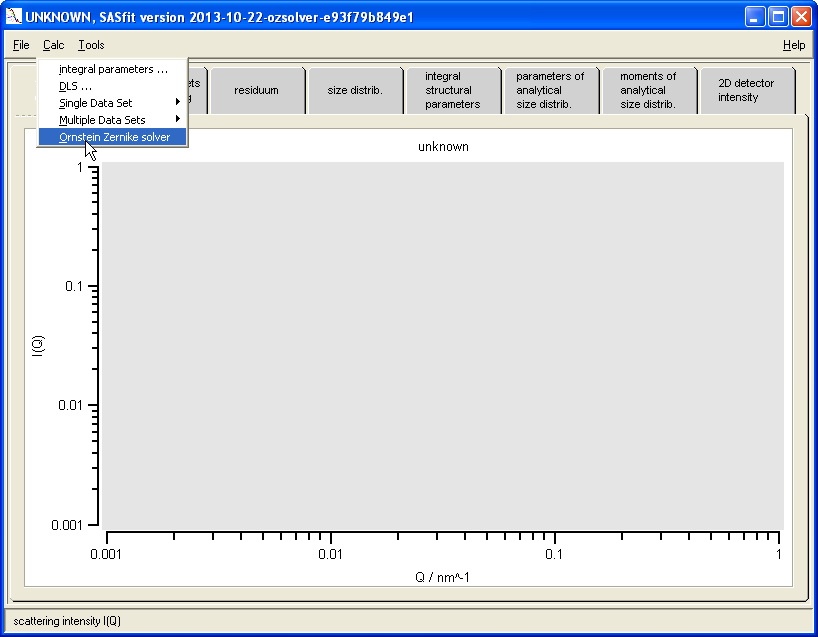
\includegraphics[width=0.708\textwidth,height=0.5\textwidth]{../images/OZsolver/startOZsolver.png}
\end{center}
\caption{Starting the menu for OZ-solver. }
\label{fig:startOZsolver}
\end{figure}

\begin{figure}[htb]
\begin{center}
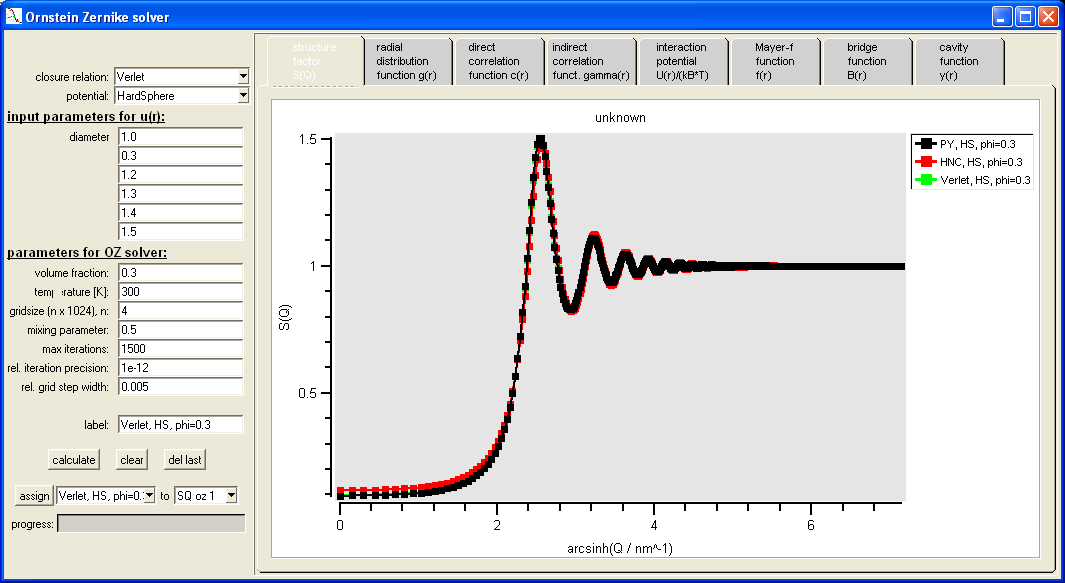
\includegraphics[width=0.913\textwidth,height=0.5\textwidth]{../images/OZsolver/mainGUIozSolver.png}
\end{center}
\caption{Main GUI for solving the Ornstein Zernike equation. }
\label{fig:mainGUIozSolver}
\end{figure}


\begin{figure}[htb]
\begin{center}
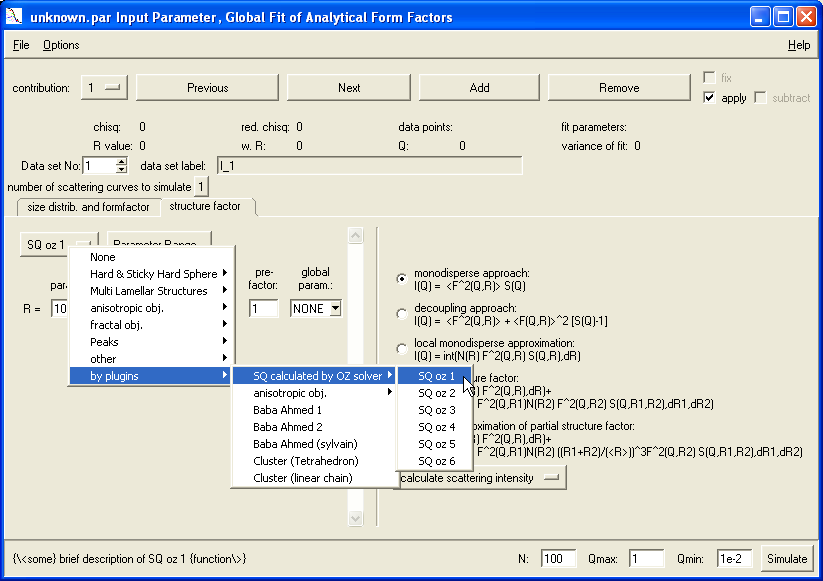
\includegraphics[width=0.708\textwidth,height=0.5\textwidth]{../images/OZsolver/OZsolverResults4fitting.png}
\end{center}
\caption{Access to the solutions of the OZ-solver.}
\label{fig:OZsolverResults4fitting}
\end{figure}
